\documentclass[11pt]{book}
\usepackage{geometry} 
\geometry{letterpaper}

\usepackage{graphicx}	
\usepackage{amssymb, amsmath}
\usepackage{subfigure}
\usepackage[table]{xcolor}
\usepackage{wasysym}
\usepackage{tikz}
\usepackage[colorlinks,linkcolor=blue,citecolor=blue,urlcolor=blue]{hyperref}

\usetikzlibrary{intersections, backgrounds, calc}

\definecolor{light}{RGB}{220, 188, 188}
\definecolor{mid}{RGB}{185, 124, 124}
\definecolor{dark}{RGB}{143, 39, 39}
\definecolor{highlight}{RGB}{0, 255, 0}
\definecolor{gray60}{gray}{0.6}
\definecolor{gray70}{gray}{0.7}
\definecolor{gray80}{gray}{0.8}
\definecolor{gray90}{gray}{0.9}
\definecolor{gray95}{gray}{0.95}

\newcommand{\dd}{ \mathrm{d} }
\newcommand{\DD}{ \mathcal{D} }
\newcommand{\PP}{ \mathbb{P} }
\newcommand{\EE}{ \mathbb{E} }
\newcommand{\RR}{ \mathbb{R} }
\newcommand{\EV}[1]{\ensuremath { \mathcal{E} \! \left( #1 \right)  } }
\newcommand{\bt}{ \mbox{\boldmath{$\theta$}} }

\usepackage[T1]{fontenc}
\usepackage{titlesec, blindtext, color}

\newcommand{\hsp}{\hspace{20pt}}
\titleformat{\chapter}[hang]{\Huge\bfseries}{\thechapter\hsp\textcolor{gray80}{|}\hsp}{0pt}{\Huge \bfseries }

\newcommand{\introversion}{0.0.0}

\graphicspath{{figures/}}

\begin{document}

\pagestyle{plain}

\frontmatter
\thispagestyle{empty}

{ \Huge \noindent Logic, Probability, and Bayesian Inference:}

\vspace{1mm}

{ \LARGE \noindent A Conceptual Introduction to the Foundations }

\vspace{1mm}

{ \LARGE \noindent of Applied Inference for Scientists and Engineers }

\vspace{5mm}

\begin{center}

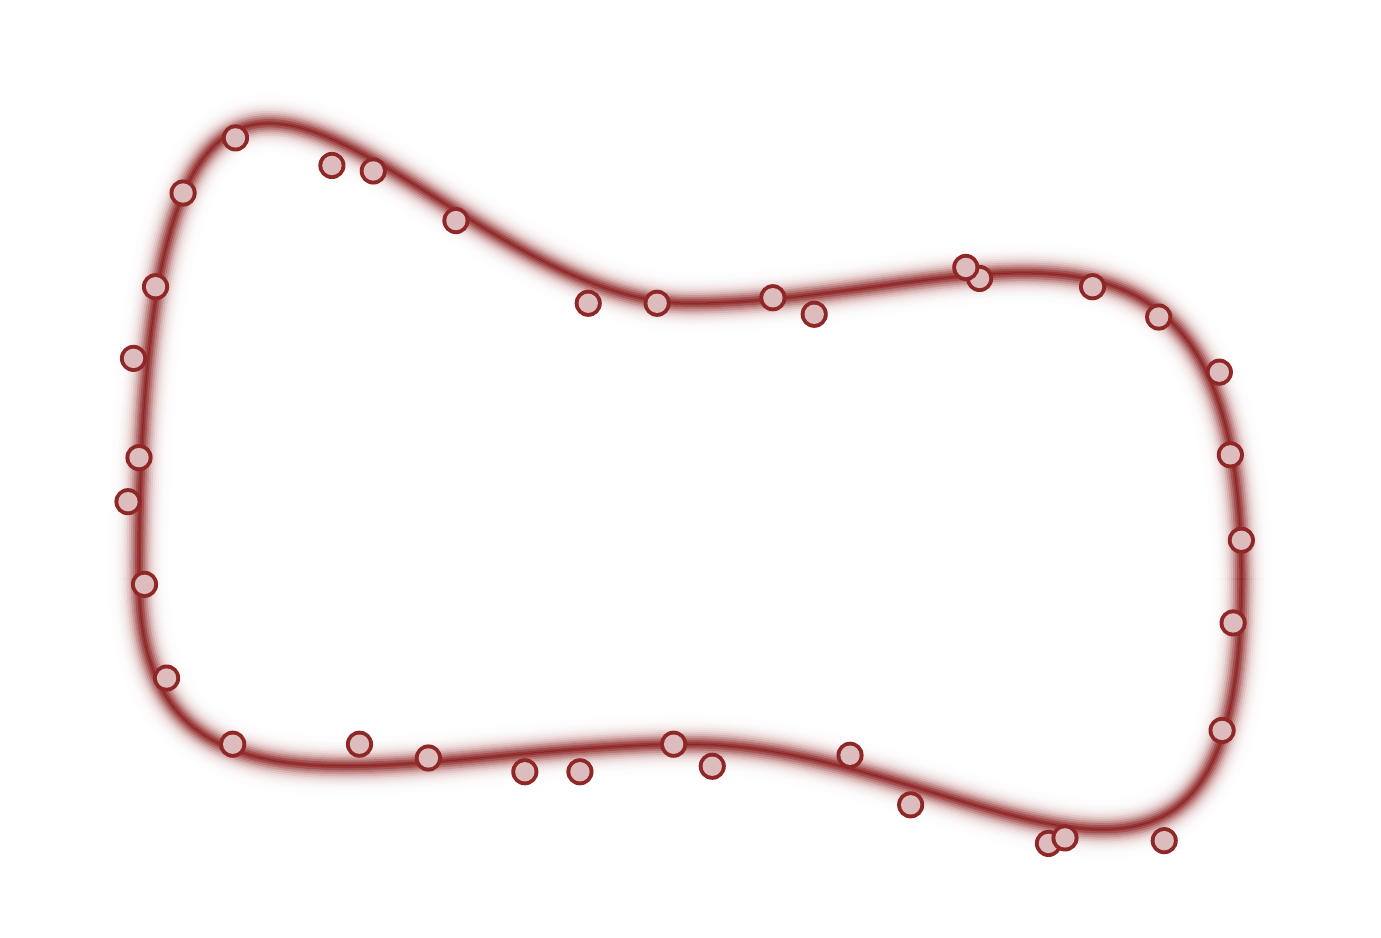
\begin{tikzpicture}[scale=0.7, thick]
  \draw[-,color=white] (-12, 0) to (12, 0);
  
  \begin{scope}
  \clip (-12, -6) rectangle (12, 10);
  \foreach \i in {0, 0.05,..., 1} {
    \draw[line width={30 * \i}, opacity={exp(-8 * \i)}, dark] 
      (-10, 0) .. controls (-10, 15) and (-5, 5) .. (0, 5)
      .. controls (5, 5) and (10, 8) .. (10, 0)
      .. controls (10, -8) and (5, -3) .. (0, -3)
      .. controls (-5, -3) and (-10, -5) .. (-10, 0);
  }
  
  \fill[color=dark] (-6, -3) circle (7pt);  
  \fill[color=light] (-6, -3) circle (5pt);
  
  \fill[color=dark] (-4.75, -3.25) circle (7pt);  
  \fill[color=light] (-4.75, -3.25) circle (5pt);
  
  \fill[color=dark] (-3, -3.5) circle (7pt);  
  \fill[color=light] (-3, -3.5) circle (5pt);
  
  \fill[color=dark] (-2, -3.5) circle (7pt);  
  \fill[color=light] (-2, -3.5) circle (5pt);
  
  \fill[color=dark] (-0.3, -3) circle (7pt);  
  \fill[color=light] (-0.3, -3) circle (5pt);  
  
  \fill[color=dark] (0.4, -3.4) circle (7pt);  
  \fill[color=light] (0.4, -3.4) circle (5pt);
  
  \fill[color=dark] (2.9, -3.2) circle (7pt);  
  \fill[color=light] (2.9, -3.2) circle (5pt);
  
  \fill[color=dark] (4, -4.1) circle (7pt);  
  \fill[color=light] (4, -4.1) circle (5pt);
  
  \fill[color=dark] (6.5, -4.8) circle (7pt);  
  \fill[color=light] (6.5, -4.8) circle (5pt);
  
  \fill[color=dark] (6.8, -4.7) circle (7pt);  
  \fill[color=light] (6.8, -4.7) circle (5pt);
  
  \fill[color=dark] (8.6, -4.75) circle (7pt);  
  \fill[color=light] (8.6, -4.75) circle (5pt);
  
  \fill[color=dark] (9.65, -2.75) circle (7pt);  
  \fill[color=light] (9.65, -2.75) circle (5pt);
  
  \fill[color=dark] (9.85, -0.8) circle (7pt);  
  \fill[color=light] (9.85, -0.8) circle (5pt);
  
  \fill[color=dark] (10, 0.7) circle (7pt);  
  \fill[color=light] (10, 0.7) circle (5pt);
  
  \fill[color=dark] (9.8, 2.25) circle (7pt);  
  \fill[color=light] (9.8, 2.25) circle (5pt);
  
  \fill[color=dark] (9.6, 3.75) circle (7pt);  
  \fill[color=light] (9.6, 3.75) circle (5pt);
  
  \fill[color=dark] (8.5, 4.75) circle (7pt);  
  \fill[color=light] (8.5, 4.75) circle (5pt);

  \fill[color=dark] (7.3, 5.3) circle (7pt);  
  \fill[color=light] (7.3, 5.3) circle (5pt);
  
  \fill[color=dark] (5.25, 5.45) circle (7pt);  
  \fill[color=light] (5.25, 5.45) circle (5pt);
  
  \fill[color=dark] (5, 5.65) circle (7pt);  
  \fill[color=light] (5, 5.65) circle (5pt);
  
  \fill[color=dark] (2.25, 4.8) circle (7pt);  
  \fill[color=light] (2.25, 4.8) circle (5pt);
  
  \fill[color=dark] (1.5, 5.1) circle (7pt);  
  \fill[color=light] (1.5, 5.1) circle (5pt);
  
  \fill[color=dark] (-0.6, 5) circle (7pt);  
  \fill[color=light] (-0.6, 5) circle (5pt);
  
  \fill[color=dark] (-1.85, 5) circle (7pt);  
  \fill[color=light] (-1.85, 5) circle (5pt);
  
  \fill[color=dark] (-4.25, 6.5) circle (7pt);  
  \fill[color=light] (-4.25, 6.5) circle (5pt);

  \fill[color=dark] (-5.75, 7.4) circle (7pt);  
  \fill[color=light] (-5.75, 7.4) circle (5pt);
  
  \fill[color=dark] (-6.5, 7.5) circle (7pt);  
  \fill[color=light] (-6.5, 7.5) circle (5pt);
  
  \fill[color=dark] (-8.25, 8) circle (7pt);  
  \fill[color=light] (-8.25, 8) circle (5pt);
  
  \fill[color=dark] (-9.2, 7) circle (7pt);  
  \fill[color=light] (-9.2, 7) circle (5pt);
  
  \fill[color=dark] (-9.7, 5.3) circle (7pt);  
  \fill[color=light] (-9.7, 5.3) circle (5pt);
  
  \fill[color=dark] (-10.1, 4) circle (7pt);  
  \fill[color=light] (-10.1, 4) circle (5pt);
  
  \fill[color=dark] (-10, 2.2) circle (7pt);  
  \fill[color=light] (-10, 2.2) circle (5pt);  
  
  \fill[color=dark] (-10.2, 1.4) circle (7pt);  
  \fill[color=light] (-10.2, 1.4) circle (5pt);  

  \fill[color=dark] (-9.9, -0.1) circle (7pt);  
  \fill[color=light] (-9.9, -0.1) circle (5pt);  

  \fill[color=dark] (-9.5, -1.8) circle (7pt);  
  \fill[color=light] (-9.5, -1.8) circle (5pt);  

  \fill[color=dark] (-8.3, -3) circle (7pt);  
  \fill[color=light] (-8.3, -3) circle (5pt);  
  
  \end{scope}
\end{tikzpicture}

\vfill

{ \Large

The Stan Development Team

Version \introversion

\today

\url{https://github.com/betanalpha/stan_intro}

}

\end{center}

\newpage
\thispagestyle{empty}

\mbox{}
\vfill


\noindent Stan Development Team. 2016  
{\it  An Technical Introduction to Probability and Bayesian Inference for Stan Users}. Version \introversion

\vspace{5mm}

\noindent Copyright \copyright \ 2016, Stan Development Team.

\vspace{5mm}

\noindent This document is distributed under the Creative Commons Attribution-NonCommercial-ShareAlike 
4.0 International License. (CC BY-NC-SA 4.0).  For full details, see

\begin{center}
\url{https://creativecommons.org/licenses/by/4.0/legalcode} 
\end{center}

\tableofcontents
\chapter*{Preface}
\addcontentsline{toc}{chapter}{Preface}

Naturally curious as a species, we all have a strong intuition
for how we can better understand the world around us.  We
first make observations and then try to gleam insight from 
those observations.  Formalizing this intuition into a robust
methodology for inference, however, is a delicate process.

Consider, for example, a ball flying through the air, slowly 
falling under the force of gravity.  After diligently recording the 
positions of the ball over its trajectory we want to identify a 
physical model that quantitatively describes its motion.  Perfect
position measurements would strongly constraint the possible
models, allowing us to exactly recover not only the trajectory 
taken by the ball but also any latent model parameters, such as 
the acceleration due to gravity, $g$ (Figure \ref{fig:motivating_example}a).  

Of course we cannot make perfect measurements in practice.
The observations we can make are limited by an inherent variability 
that obscures the underlying trajectory; multiple trajectories, and
hence multiple physical models, are all consistent with the noisy
measurements (Figure \ref{fig:motivating_example}b).  In order
to learn from these realistic measurements we need not only 
models of the ball's motion and models of the variability in the
measurements, but also a means of quantifying the uncertainty
in which of those models are consistent with the observations.
\emph{The only conclusive statement we can make is how uncertain 
we are.}

\begin{figure*}
\centering
\subfigure[]{
\begin{tikzpicture}[scale=0.25, thick]
  \draw[dashed, rotate=180, color=gray70] (0, -10) parabola (-20, 0);

  \fill[color=dark] (2, -0.025 * 2 * 2 + 10) circle (7pt);  
  \fill[color=light] (2, -0.025 * 2 * 2 + 10) circle (5pt);  
  
  \fill[color=dark] (5, -0.025 * 5 * 5 + 10) circle (7pt);  
  \fill[color=light] (5, -0.025 * 5 * 5 + 10) circle (5pt);  
  
  \fill[color=dark] (7, -0.025 * 7 * 7 + 10) circle (7pt);  
  \fill[color=light] (7, -0.025 * 7 * 7 + 10) circle (5pt);  
  
  \fill[color=dark] (10, -0.025 * 10 * 10 + 10) circle (7pt);  
  \fill[color=light] (10, -0.025 * 10 * 10 + 10) circle (5pt);  
  
  \fill[color=dark] (13, -0.025 * 13 * 13 + 10) circle (7pt);  
  \fill[color=light] (13, -0.025 * 13 * 13 + 10) circle (5pt);  
  
  \fill[color=dark] (14, -0.025 * 14 * 14 + 10) circle (7pt);  
  \fill[color=light] (14, -0.025 * 14 * 14 + 10) circle (5pt);  
  
  \fill[color=dark] (17, -0.025 * 17 * 17 + 10) circle (7pt);  
  \fill[color=light] (17, -0.025 * 17 * 17 + 10) circle (5pt);  
  
  \fill[color=dark] (18, -0.025 * 18 * 18 + 10) circle (7pt);  
  \fill[color=light] (18, -0.025 * 18 * 18 + 10) circle (5pt);  

  \fill[color=dark] (19, -0.025 * 19 * 19 + 10) circle (7pt);  
  \fill[color=light] (19, -0.025 * 19 * 19 + 10) circle (5pt);  
  
  \draw[->] (22, 13) node[above] {$g$} -- (22, 10);
      
  \draw[->] (0, 0) -- (25,0) node[right] {$x$};
  \draw[->] (0, 0) -- (0,15) node[above] {$y$};
\end{tikzpicture}
}
\subfigure[]{
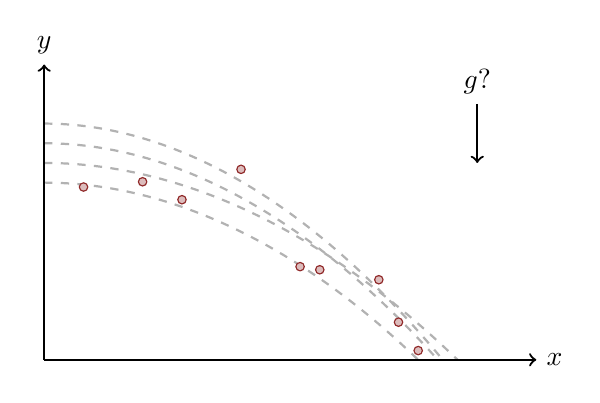
\begin{tikzpicture}[scale=0.25, thick]
  \draw[dashed, rotate=180, color=gray70] (0, -9) parabola (-19, 0);
  \draw[dashed, rotate=180, color=gray70] (0, -11) parabola (-20, 0);
  \draw[dashed, rotate=180, color=gray70] (0, -12) parabola (-20.25, 0);
  \draw[dashed, rotate=180, color=gray70] (0, -10) parabola (-21, 0);

  \fill[color=dark] (2, -0.025 * 2 * 2 + 10 -1.123067470) circle (7pt);  
  \fill[color=light] (2, -0.025 * 2 * 2 + 10 -1.123067470) circle (5pt);  
  
  \fill[color=dark] (5, -0.025 * 5 * 5 + 10 -0.330845947) circle (7pt);  
  \fill[color=light] (5, -0.025 * 5 * 5 + 10 -0.330845947) circle (5pt);  
  
  \fill[color=dark] (7, -0.025 * 7 * 7 + 10 -0.642779020) circle (7pt);  
  \fill[color=light] (7, -0.025 * 7 * 7 + 10 -0.642779020) circle (5pt);  
  
  \fill[color=dark] (10, -0.025 * 10 * 10 + 10 + 2.174536596) circle (7pt);  
  \fill[color=light] (10, -0.025 * 10 * 10 + 10 + 2.174536596) circle (5pt);  
  
  \fill[color=dark] (13, -0.025 * 13 * 13 + 10 -1.043929042) circle (7pt);  
  \fill[color=light] (13, -0.025 * 13 * 13 + 10 -1.043929042) circle (5pt);  
  
  \fill[color=dark] (14, -0.025 * 14 * 14 + 10 -0.526778959) circle (7pt);  
  \fill[color=light] (14, -0.025 * 14 * 14 + 10 -0.526778959) circle (5pt);  
  
  \fill[color=dark] (17, -0.025 * 17 * 17 + 10 + 1.290826126) circle (7pt);  
  \fill[color=light] (17, -0.025 * 17 * 17 + 10 + 1.290826126) circle (5pt);  
  
  \fill[color=dark] (18, -0.025 * 18 * 18 + 10 + 0.008352532) circle (7pt);  
  \fill[color=light] (18, -0.025 * 18 * 18 + 10 + 0.008352532) circle (5pt);  

  \fill[color=dark] (19, -0.025 * 19 * 19 + 10 -0.508723224) circle (7pt);  
  \fill[color=light] (19, -0.025 * 19 * 19 + 10 -0.508723224) circle (5pt);  
  
  \draw[->] (22, 13) node[above] {$g?$} -- (22, 10);
      
  \draw[->] (0, 0) -- (25,0) node[right] {$x$};
  \draw[->] (0, 0) -- (0,15) node[above] {$y$};
\end{tikzpicture}
}
\caption{(a) Perfect measurements of a ball falling under the influence
of gravity would strongly constrain any physical model of that motion, 
including latent parameters such as the the strength of gravity, $g$.
(b) In practice, however, measurements are inherently variable, which 
limits our ability to infer the exact trajectory and hence any model of how 
the trajectory itself.  Here and in all measurements, uncertainty is intrinsic 
to learning.}
\label{fig:motivating_example}
\end{figure*}

This simple example demonstrates a intrinsic principle that underlies 
science, industry, medicine, and any other field that attempts to learn from
observations: uncertainty is inherent to learning and decision making.
In particular, if we want to develop any formal methodology for inference
and decision making then we first need a formal procedure for quantifying
and manipulating uncertainty itself.  \emph{Bayesian inference} uses 
\emph{probability theory} to quantify all forms of uncertainty, including not 
only the intrinsic variability of measurements but also ignorance in the 
learning process itself.  This unified perspective provides an elegant and
powerful approach for first making inferences and then making robust
decisions.

\section{Our Objectives}

While reading this review we want the reader to learn how probability 
theory can be used to quantify uncertainty both in theory and in practice,
ultimately motivating Bayesian inference itself.  Unfortunately, this seemingly 
straightforward objective ends up being quickly complicated by the subtle 
and often counterintuitive nature of probability theory itself.  

Many introductory treatments of Bayesian inference ignore these subtleties
entirely, oversimplifying the subject and neglecting many of its finer technical 
aspects.  Unfortunately, these technicalities are not irrelevant -- indeed they
often have a strong influence on practical applications of  the theory.  Without 
at least a conceptual understanding of these technicalities, the readier is then 
subject to dangerous fallacies and, ultimately, fragile analyses.  

On the other hand, the more formal treatments of probability theory that do 
address these subtleties are typically mired in abstract, mathematical pedantry 
with little or not discussion of how the theory applies to inference.  A few
treatments will introduce the application of these ideas to frequentist inference,
but rarely is there any discussion of the more general Bayesian perspective.

In this review we attempt an intermediate treatment where we provide a deeper 
introduction to probability theory and Bayesian inference than most introductory
references, but focus entirely on concepts rather than proofs.  We hope that
this will give Stan users the foundational understanding they need to properly 
wield Bayesian inference in practice and take full advantage of their measurements.

\section{Our Strategy}

Probability theory, like much of higher mathematics, is challenging because
of its abstraction; the theory is defined in complete generality with only abstract 
objects and manipulations.  While much can be proved about the behavior
of these abstractions, there is no general way to explicitly specify these objects 
and implement their manipulations.  Without explicit examples it then becomes
difficult to develop accurate intuition and understanding.

To apply probability theory in practice we need to first define a \emph{representation} 
that maps these abstractions into an explicit context where we can compute.  
For example, we can map into a discrete space where manipulations reduce 
to counting or a real space where manipulations reduce to integration.  The 
challenge in using these representations is to ensure that the calculations depend 
only on the properties of the original abstract system and not on any irrelevant details
of the representation itself.  Understanding exactly what details are relevant or 
not, however, requires at least some comprehension of the abstract theory.

Many introductions to probability and statistics simply jump into one of these 
representations immediately, ignoring the abstractions, and the subtitles as to
which operations are valid, altogether.  This approach inevitably leads to 
confused frustration.  \emph{What do you mean a probability \emph{density} isn't
a probability?  What do you mean most observations won't be near the mode
of the probability density?}.  Unfortunately, this confusion manifests not just in
frustration but also incorrect statistical analyses that can have serious consequences.

In this introduction we will not ignore the abstractions of probability theory.
As with more formal treatments we will instead being by discussion the abstract
theory and only then discuss representations and the explicit computations that
they allow.   Unlike those treatments, however, our presentation will be largely
conceptual, meanings lots of definitions of abstract objects and their manipulations
but little concern for any technical details that do not end up affecting the
application of the theory in practice.  As we develop representations we'll discuss 
more and more specific examples to develop as much intuitive context as can while 
also emphasizing the limitations of these representations.

We'll first introduce logic as a means of quantifying information with certainty,
and then probability theory as a means of quantifying uncertainty about that 
information.  In both cases we'll first consider abstract definitions and then the 
explicit representations of these concepts needed in practice.  Next we'll discuss 
how to implement probabilistic computations and discuss many popular computational 
methods.  Finally we'll show how all of these ideas come together in Bayesian 
inference.

This will not be an easy journey.  It requires a significant investment from the 
reader, but that investment will be rewarded with a robust understanding of 
statistics that will enable some amazing science. 

\section{Mathematical Background and Notation}

A thorough review of probability theory and its application requires a nontrivial
mathematical background.  We have attempted to make this review as
self-contained as possible regarding probability theory itself, but we do have to 
assume that the reader is comfortable with the basics of set theory and differential 
and integral calculus over the real numbers.  We highly encourage anyone whose 
math might be rusty to brush up before proceeding.

Throughout we will use common set theory notation.  If $A$ is a set
then any element of the set is written as $a \in A$ while a subset is written
as $S \subset A$.  Sets are also sometimes denoted by their elements, for
example $A = \left\{ a_{1}, \ldots, a_{N} \right\}$.  The \emph{set builder
notation} is similarly used to denote subsets as 
$S = \left\{ a \in A \mid \cdot \right\}$, where $\cdot$ is the condition identifying
which elements of $A$ are in the subset $S \subset A$.  For example, we
can define the positive real numbers as 
%
\begin{equation*}
\RR^{+} = \left\{ x \in \RR \mid x \ge 0 \right\}.
\end{equation*}
%
The \emph{union} of two sets, $A \cup B$ is the combination of all 
elements in either set while the \emph{intersection} of two sets, 
$A \cap B$ contains only those elements that appear in both sets.
If $S \subset A$ is a subset then its \emph{complement}, $S^{c}$ is 
the collection of all elements of $A$ not in $S$.

\emph{Spaces} are sets endowed with a structure called a 
\emph{topology} that allows us to separate ``well-behaved subsets''
from ``pathological subsets''.  We will assume that all of our sets
have such a structure and consequently for all intents and purposes 
set and space will be used interchangeably.  Topologies are also
useful for characterizing spaces.  For example, the familiar properties
of discrete spaces and continuous spaces, such as the real numbers, 
are defined are defined by their respective topologies.

Throughout we will use the common notation for maps from one set into 
another, $f : A \rightarrow B$ which defines $f$ as a map taking elements 
of the set $A$ to elements of the set $B$. In other words, $f(a) \in B$ for 
any $a \in A$.  Sometimes we will be more explicit regarding the action
on a given point and write
%
\begin{align*}
f &: A \rightarrow B \\
  &\quad a \mapsto f \! \left( a \right).
\end{align*}

At times we will be less precise.  For example, when discussing computation 
we will liberally use $\approx$ to define when two objects are approximately 
equal, or when we \emph{assume} that they are approximately equal, without 
making any effort to formally define what ``approximately equal'' means.
Similarly, we will make no attempt at the full mathematical rigor necessary for 
a complete understanding of the intricacies of probability theory, and instead 
focus on developing a high-level, conceptual intuition.  In particular, in many 
places we will appeal to vague notions like ``well-behaved'', as their technical 
definitions do not offer much pedagogical benefit.



\mainmatter
\chapter{Logic}

Before we can formalize \emph{learning} about the world around us we 
first need a formal means of \emph{describing} the world.  \emph{Logical 
propositions} provide a mathematically-precise language for quantifying
information about a system with certainty.  In this section we will review 
abstract logical propositions, their manipulations, and how we can 
represent them in practice.  We conclude with a brief discussion of 
implicative statements.

\section{Logical Propositions}

If $\mathcal{S}$ is an abstract system of interest then any description of 
$\mathcal{S}$ can be defined as a \emph{logical proposition} which asserts
that a statement about that system is either true or false.  For example, 
consider describing one of the eight planets in our Solar System: Mercury 
($\mercury$), Venus ($\venus$), Earth ($\earth$), Mars ($\mars$), Jupiter 
($\jupiter$), Saturn ($\saturn$), Uranus ($\uranus$), and Neptune ($\neptune$).  
Information about the planet is encapsulated in logical propositions asserting
both statements that are true, for example
%
\begin{equation*}
P_{1} = \text{``the planet has an atmosphere''},
\end{equation*}
%
and statements that are false, for example
\begin{equation*} 
P_{2}=\text{``the planet does not have rings''}.
\end{equation*} 

Logical propositions can be manipulated into other logical propositions
with any of three \emph{boolean operations} (Table 
\ref{tab:boolean_truth_tables}).  \emph{Negatation}, $\neg$, is a unary 
operator resulting in a proposition asserting the converse of the input 
proposition: 
%
\begin{equation*}
\neg P_{1}=\text{``the planet does \emph{not} have an atmosphere''}.
\end{equation*}
%
Binary operations take propositions about two statements and define 
a new proposition about the joint statement.  The result of a 
\emph{conjunction}, $\wedge$, is true only when both input propositions 
are true:
%
\begin{equation*}
P_{1} \wedge P_{2} =
 \text{``the planet does not has both an atmosphere and rings''}.  
\end{equation*}
%
A \emph{disjunction}, $\vee$, however, is true whenever either input 
proposition is true : 
%
\begin{equation*}
P_{1} \vee P_{2} =
\text{``the planet does have an atmosphere \emph{or} rings''}.
\end{equation*}

\begin{table}
  \centering
  \renewcommand{\arraystretch}{1.5}
  \begin{tabular}{cc}
    \rowcolor[gray]{0.9} 
    \multicolumn{2}{c}{\textbf{Negation}} \\
    %
    \rowcolor[gray]{0.9} 
    $P$ & $\neg P$ \\
    %
    False & True \\
    True & False \\
  \end{tabular}
  %
  \vspace{3mm} \\
  %
  \begin{tabular}{ccc}
    \rowcolor[gray]{0.9} 
    \multicolumn{3}{c}{\textbf{Conjunction}} \\
    %
    \rowcolor[gray]{0.9} 
    $P_{1}$ & $P_{2}$ & $P_{1} \wedge P_{2}$ \\
    %
    False & False & False \\
    True & False & False \\
    False & True & False \\
    True & True & True \\
  \end{tabular}
  %
  \hspace{5mm}
  %
  \begin{tabular}{ccc}
    \rowcolor[gray]{0.9} 
    \multicolumn{3}{c}{\textbf{Disjunction}} \\
    %
    \rowcolor[gray]{0.9} 
    $P_{1}$ & $P_{2}$ & $P_{1} \vee P_{2}$ \\
    %
    False & False & False \\
    True & False & True \\
    False & True & True \\
    True & True & True \\
  \end{tabular}
\caption{The three basic Boolean operations transform given
logical propositions into new logical propositions, and their 
action is conveniently summarized in truth tables.}
\label{tab:boolean_truth_tables}
\end{table}

Naively, we might think that a system would be completely described only 
once we have defined a proposition for every statement, classifying each 
as either true or false. In his infamous Incompleteness Theorems, however, 
G\"{o}del showed that if we try to define a proposition for every possible 
statement about $\mathcal{S}$ then there will exist some pathological 
propositions that are not consistent with the Boolean operations.  For 
example, there are always pathological propositions asserting truth whose 
negations do not assert falseness!  These pathological propositions cannot 
be explicitly constructed in practice, only proven to exist, but in order to 
ensure a self-consistent description of the system we need some means of 
removing them.

To avoid these pathological propositions we leverage the fact that propositions
about non-pathological statements yield non-pathological propositions when 
we apply any Boolean operation.  In other words, well-behaved propositions 
are \emph{closed} under these operations, and any collection of well-behaved, 
consistent propositions forms a logical algebra, 
$\mathcal{L} \! \left( \mathcal{S} \right)$.  

We will refer to the pairing of an abstract system with some choice of a logical
algebra as a \emph{logical model}, 
$\left( \mathcal{S}, \mathcal{L} \! \left( \mathcal{S} \right) \right)$.

\section{Representations of Logical Models}

Logical models provide a very abstract, and hence very genetic, framework for 
describing arbitrary systems, but that abstraction also makes these descriptions
ungainly to specify and manipulate in practice.  For our abstract descriptions to 
be useful we need an explicit language in which we can communicate them, 
which we will refer to as a \emph{representation} 
(Table \ref{tab:representation_examples}).

\begin{table}
  \centering
  \renewcommand{\arraystretch}{1.5}
  \begin{tabular}{ccc}
    \rowcolor[gray]{0.9} 
    \textbf{Abstract System} & \textbf{Representation} & \textbf{Measurable Maps} \\
    %
    Historical Decrees & Ancient Languages & Translations \\
    & (Egyptian, Demotic, Green, $\ldots$) & (Rosetta Stone) \\
    % 
    Computer Program & Programming Languages & Source-to-Source \\
    & (C++, S, Python, $\ldots$) & Compilers \\
    %
    Unordered Categories & Integers & Permutations \\
    %
    Direction & Vector Space & Changes of Basis \\
    %
    Position & Coordinates & Reparameterizations \\
    %
    Quantification & Units & Changes of Units \\
  \end{tabular}
\caption{Representations provide a concrete language in which we can
communicate the descriptions of an abstract system.  Because there 
are many degenerate ways to express these descriptions, these 
representations are not unique and in practice we have to be careful 
that the irrelevant details of any particular representation do not affect
the descriptions themselves.}
\label{tab:representation_examples}
\end{table}

In order to construct a representation we assume that the properties
of our abstract system take values in some \emph{sample space}, 
$\Theta$, such as integers or real numbers.  Statements about these
properties are represented as subsets of the sample space, and
logical propositions are represented as set inclusion.  If a statement
is represented by $E \subset \Theta$, for example, then a logical
proposition asserting that the statement is true is represented by 
asserting that $\theta \in E$, and one asserting that the statement
is false is represented by asserting that $\theta \notin E$.

With propositions represented by set inclusion and set exclusion,
the Boolean operations are naturally implemented with set operations.  
Conjunction becomes inclusion in the subset intersection, disjunction 
inclusion in the subset union, and negation inclusion in the subset 
complement negation (Figure \ref{fig:venn_diagrams}, 
Table \ref{tab:set_truth_tables}).  

\begin{figure*}
\centering
\subfigure[]{
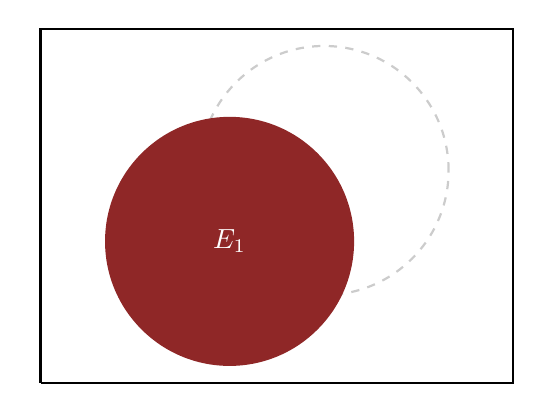
\begin{tikzpicture}[scale=0.3, thick]
  \draw[color=white] (-0.5, 0) to (20.5, 0);
  \draw[color=black] (0, 0) to (20, 0) to (20, 15) to (0, 15) to (0, 0);
  \draw[color=gray80, dashed] (12, 9) circle (150pt); 
  \fill[color=dark] (8, 6) circle (150pt) node[color=white] {$E_{1}$}; 
\end{tikzpicture}
%
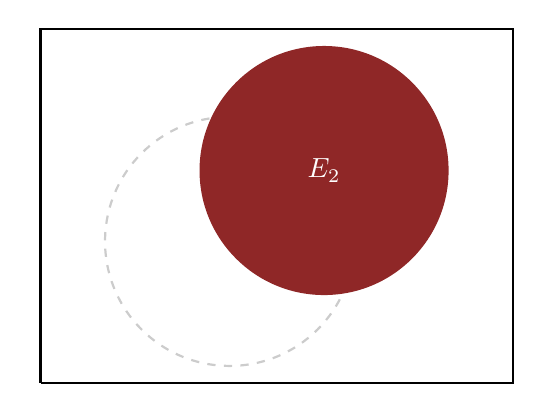
\begin{tikzpicture}[scale=0.3, thick]
  \draw[color=white] (-0.5, 0) to (20.5, 0);
  \draw[color=black] (0, 0) to (20, 0) to (20, 15) to (0, 15) to (0, 0);
  \draw[color=gray80, dashed] (8, 6) circle (150pt); 
  \fill[color=dark] (12, 9) circle (150pt) node[color=white] {$E_{2}$}; 
\end{tikzpicture}
}
%
\subfigure[]{
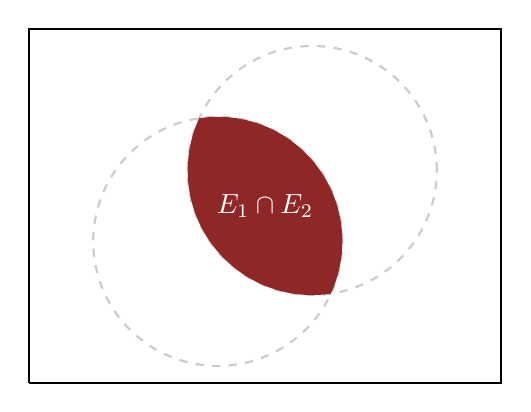
\begin{tikzpicture}[scale=0.3, thick]
  \draw[color=black] (0, 0) to (20, 0) to (20, 15) to (0, 15) to (0, 0);
  \draw[color=gray80, dashed] (8, 6) circle (150pt); 
  \draw[color=gray80, dashed] (12, 9) circle (150pt); 
  \begin{scope}
    \clip (8, 6) circle (150pt);
    \fill[color=dark] (12, 9) circle (150pt); 
  \end{scope}
  \node[color=white] at (10, 7.5) {$E_{1} \cap E_{2}$};
\end{tikzpicture}
}
%
\subfigure[]{
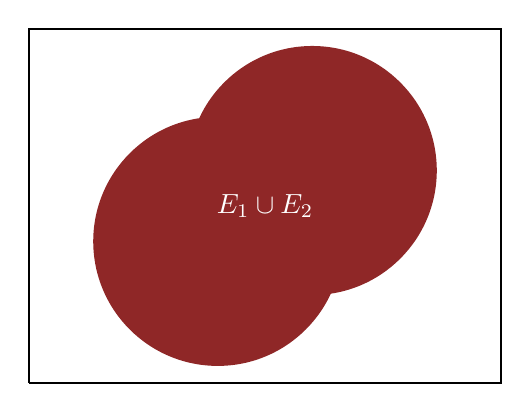
\begin{tikzpicture}[scale=0.3, thick]
  \draw[color=black] (0, 0) to (20, 0) to (20, 15) to (0, 15) to (0, 0);
  \fill[color=dark] (8, 6) circle (150pt); 
  \fill[color=dark] (12, 9) circle (150pt); 
  \node[color=white] at (10, 7.5) {$E_{1} \cup E_{2}$};
\end{tikzpicture}
}
%
\subfigure[]{
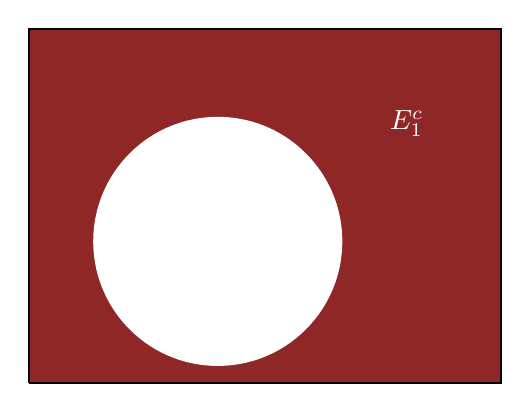
\begin{tikzpicture}[scale=0.3, thick]
  \fill[color=dark] (0, 0) to (20, 0) to (20, 15) to (0, 15) to (0, 0);
  \draw[color=black] (0, 0) to (20, 0) to (20, 15) to (0, 15) to (0, 0);
  \fill[color=white] (8, 6) circle (150pt); 
  \node[color=white] at (16, 11) {$E_{1}^{c}$};
\end{tikzpicture}
}
%
\caption{In a representation statements are defined as subsets in some
sample space and logical propositions are implemented with set inclusion
or set exclusion.  Boolean operations are then implemented with inclusion
in a set complement (negation), set intersection (conjunction), and set
union (disjunction).  (a) If two propositions are represented by
inclusion in the sets $E_{1}$ and $E_{2}$, then (b) their conjunction is 
represented as inclusion in the set intersection, $E_{1} \cup E_{2}$, and (c) 
their disjunction is represented as inclusion in the set union, 
$E_{1} \cap E_{2}$.  (d) Similarly, the negation of $E_{1}$ is represented
as inclusion in the set complement, $E_{1}^{c}$.}
\label{fig:venn_diagrams}
\end{figure*}

\begin{table}
  \centering
  \renewcommand{\arraystretch}{1.5}
  \begin{tabular}{cc}
    \rowcolor[gray]{0.9} 
    \multicolumn{2}{c}{\textbf{Negation}} \\
    %
    \rowcolor[gray]{0.9} 
    $\theta \in E$ & $\theta \in E^{c}$ \\
    %
    False & True \\
    True & False \\
  \end{tabular}
  %
  \vspace{3mm} \\
  %
  \begin{tabular}{ccc}
    \rowcolor[gray]{0.9} 
    \multicolumn{3}{c}{\textbf{Conjunction}} \\
    %
    \rowcolor[gray]{0.9} 
    $\theta \in E_{1}$ & $\theta \in E_{1}$ & $\theta \in E_{1} \cap E_{2}$ \\
    %
    False & False & False \\
    True & False & False \\
    False & True & False \\
    True & True & True \\
  \end{tabular}
  %
  \hspace{5mm}
  %
  \begin{tabular}{ccc}
    \rowcolor[gray]{0.9} 
    \multicolumn{3}{c}{\textbf{Disjunction}} \\
    %
    \rowcolor[gray]{0.9} 
    $\theta \in E_{1}$ & $\theta \in E_{1}$ & $\theta \in E_{1} \cup E_{2}$ \\
    %
    False & False & False \\
    True & False & True \\
    False & True & True \\
    True & True & True \\
  \end{tabular}
\caption{In a representation statements are defined as subsets in some
sample space and logical propositions are implemented with set inclusion
or set exclusion.  Boolean operations are then implemented with inclusion
in a set complement (negation), set intersection (conjunction), and set
union (disjunction), which yield the same truth tables and hence define
a valid representation.}
\label{tab:set_truth_tables}
\end{table}

The same inconsistencies that limited us to consider only well-behaved 
logical propositions, however, also limit our representations to only
well-behaved subsets of the sample space.  We denote a collection of 
subsets of the sample space that is closed under set compliments,
set intersections, and set unions as an \emph{event space}, $\EV{\Theta}$,
with the well-behaved subsets in that space denoted \emph{events}. 
Event spaces always include the null event, $E = \emptyset$, which 
can never be true as it is always empty.  Similarly, event spaces also 
always include the trivial event, $E = \Theta$, which can never be false
as every element of the sample space is included in this event.  
The pairing of a sample space and an event space is denoted a
\emph{measurable space}, for reasons that will become more clear
in the next chapter.

More formally, then, we should define a representation as a map from 
a logical model into a measurable space.  In practice this is defined 
as a map from the abstract system into the sample space,
%
\begin{equation*}
\mathfrak{r} : \mathcal{S} \rightarrow \Theta,
\end{equation*}
%
that then induces a map from the logical algebra into the event space,
%
\begin{equation*}
\mathfrak{r}_{*} : 
\mathcal{L} \! \left( \mathcal{S} \right) \rightarrow \EV{\Theta}.
\end{equation*}
%
A representation is called \emph{faithful} if every logical statement maps 
into an event and vice-versa, and Stone's Theorem guarantees that a
faithful representation for any logical model always exists.

For example, descriptions of the planets in our solar system can be 
represented with the integers, $\Theta = \left\{1, 2, \ldots, 8 \right\}$, 
with each logical proposition represented by inclusion in a subset of 
those integers (Figure \ref{fig:discrete_set_logic}).  Similarly, the 
distance between two objects can be represented by real numbers,
(Figure \ref{fig:real_set_logic}).

\begin{figure*}
\centering
\subfigure[]{
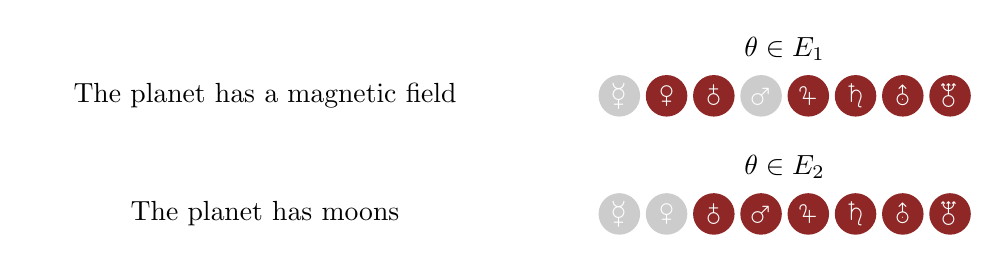
\begin{tikzpicture}[scale=0.3, thick]
  \draw[color=white] (-25, 0) to (10, 0);

  \node[] at (-15, 0) {The planet has a magnetic field};
  \node[] at (7, 2) {$\theta \in E_{1}$};

  \fill[color=gray80] (0, 0) circle (25pt) node[color=white] {$\mercury$}; 
  \fill[color=dark] (2, 0) circle (25pt) node[color=white] {$\venus$}; 
  \fill[color=dark] (4, 0) circle (25pt) node[color=white] {$\earth$}; 
  \fill[color=gray80] (6, 0) circle (25pt) node[color=white] {$\mars$}; 
  \fill[color=dark] (8, 0) circle (25pt) node[color=white] {$\jupiter$}; 
  \fill[color=dark] (10, 0) circle (25pt) node[color=white] {$\saturn$}; 
  \fill[color=dark] (12, 0) circle (25pt) node[color=white] {$\uranus$}; 
  \fill[color=dark] (14, 0) circle (25pt) node[color=white] {$\neptune$};  
  
  \node[] at (-15, -5) {The planet has moons};
  \node[] at (7, -3) {$\theta \in E_{2}$};

  \fill[color=gray80] (0, -5) circle (25pt) node[color=white] {$\mercury$}; 
  \fill[color=gray80] (2, -5) circle (25pt) node[color=white] {$\venus$}; 
  \fill[color=dark] (4, -5) circle (25pt) node[color=white] {$\earth$}; 
  \fill[color=dark] (6, -5) circle (25pt) node[color=white] {$\mars$}; 
  \fill[color=dark] (8, -5) circle (25pt) node[color=white] {$\jupiter$}; 
  \fill[color=dark] (10, -5) circle (25pt) node[color=white] {$\saturn$}; 
  \fill[color=dark] (12, -5) circle (25pt) node[color=white] {$\uranus$}; 
  \fill[color=dark] (14, -5) circle (25pt) node[color=white] {$\neptune$};  
\end{tikzpicture}
}
%
\subfigure[]{
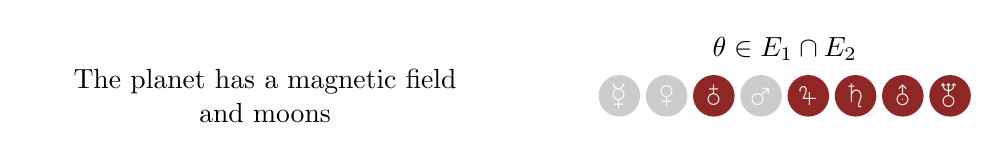
\begin{tikzpicture}[scale=0.3, thick]
  \draw[color=white] (-25, 0) to (10, 0);
  
  \node[align=center] at (-15, 0) {The planet has a magnetic field\\and moons};
  \node[] at (7, 2) {$\theta \in E_{1} \cap E_{2}$};

  \fill[color=gray80] (0, 0) circle (25pt) node[color=white] {$\mercury$}; 
  \fill[color=gray80] (2, 0) circle (25pt) node[color=white] {$\venus$}; 
  \fill[color=dark] (4, 0) circle (25pt) node[color=white] {$\earth$}; 
  \fill[color=gray80] (6, 0) circle (25pt) node[color=white] {$\mars$}; 
  \fill[color=dark] (8, 0) circle (25pt) node[color=white] {$\jupiter$}; 
  \fill[color=dark] (10, 0) circle (25pt) node[color=white] {$\saturn$}; 
  \fill[color=dark] (12, 0) circle (25pt) node[color=white] {$\uranus$}; 
  \fill[color=dark] (14, 0) circle (25pt) node[color=white] {$\neptune$};  
\end{tikzpicture}
}
%
\subfigure[]{
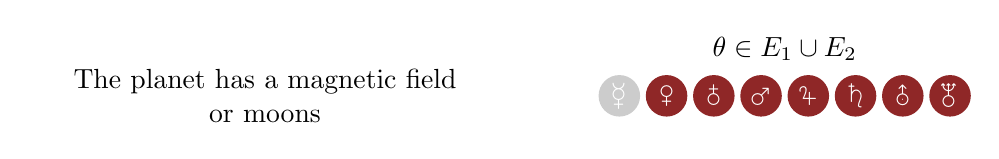
\begin{tikzpicture}[scale=0.3, thick]
  \draw[color=white] (-25, 0) to (10, 0);
   
  \node[align=center] at (-15, 0) {The planet has a magnetic field\\or moons};
  \node[] at (7, 2) {$\theta \in E_{1} \cup E_{2}$};

  \fill[color=gray80] (0, 0) circle (25pt) node[color=white] {$\mercury$}; 
  \fill[color=dark] (2, 0) circle (25pt) node[color=white] {$\venus$}; 
  \fill[color=dark] (4, 0) circle (25pt) node[color=white] {$\earth$}; 
  \fill[color=dark] (6, 0) circle (25pt) node[color=white] {$\mars$}; 
  \fill[color=dark] (8, 0) circle (25pt) node[color=white] {$\jupiter$}; 
  \fill[color=dark] (10, 0) circle (25pt) node[color=white] {$\saturn$}; 
  \fill[color=dark] (12, 0) circle (25pt) node[color=white] {$\uranus$}; 
  \fill[color=dark] (14, 0) circle (25pt) node[color=white] {$\neptune$};  
\end{tikzpicture}
}
%
\subfigure[]{
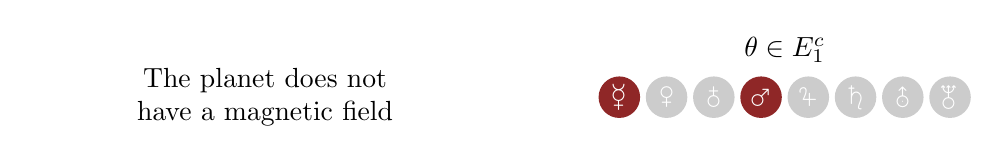
\begin{tikzpicture}[scale=0.3, thick]
  \draw[color=white] (-25, 0) to (10, 0);
   
  \node[align=center] at (-15, 0) {The planet does not\\have a magnetic field};
  \node[] at (7, 2) {$\theta \in E_{1}^{c}$};

  \fill[color=dark] (0, 0) circle (25pt) node[color=white] {$\mercury$}; 
  \fill[color=gray80] (2, 0) circle (25pt) node[color=white] {$\venus$}; 
  \fill[color=gray80] (4, 0) circle (25pt) node[color=white] {$\earth$}; 
  \fill[color=dark] (6, 0) circle (25pt) node[color=white] {$\mars$}; 
  \fill[color=gray80] (8, 0) circle (25pt) node[color=white] {$\jupiter$}; 
  \fill[color=gray80] (10, 0) circle (25pt) node[color=white] {$\saturn$}; 
  \fill[color=gray80] (12, 0) circle (25pt) node[color=white] {$\uranus$}; 
  \fill[color=gray80] (14, 0) circle (25pt) node[color=white] {$\neptune$};  
\end{tikzpicture}
}
\caption{(a) Systems that take discrete values, such as the planets in 
our solar system, can be represented with integers, with any logical 
proposition about the planets represented by inclusion in a subset of 
integers. (b) Conjuction of logical propositions is implemented with 
inclusion in set intersections, (c) disjunction with inclusion in set unions, 
and (d) negation with inclusion in set complements.}
\label{fig:discrete_set_logic}
\end{figure*}

\begin{figure*}
\centering
\subfigure[]{
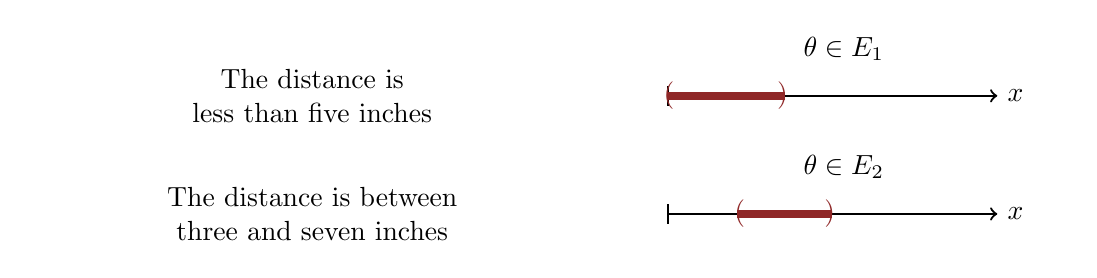
\begin{tikzpicture}[scale=0.3, thick]
  \draw[color=white] (-27, 0) to (17, 0);

  \node[align=center] at (-15, 0) {The distance is\\less than five inches};
  \node[] at (7.5, 2) {$\theta \in E_{1}$};

  \draw[|->] (0, 0) -- (14,0) node[right] {$x$};
  \draw[line width=1mm, color=dark] (0, 0) node[] {$\,($} -- (5, 0) node[] {$\!)$};
  
  \node[align=center] at (-15, -5) {The distance is between\\three and seven inches};
  \node[] at (7.5, -3) {$\theta \in E_{2}$};
  
  \draw[|->] (0, -5) -- (14,-5) node[right] {$x$};
  \draw[line width=1mm, color=dark] (3, -5) node[] {$\,($} -- (7,-5) node[] {$\!)$};

\end{tikzpicture}
}
%
\subfigure[]{
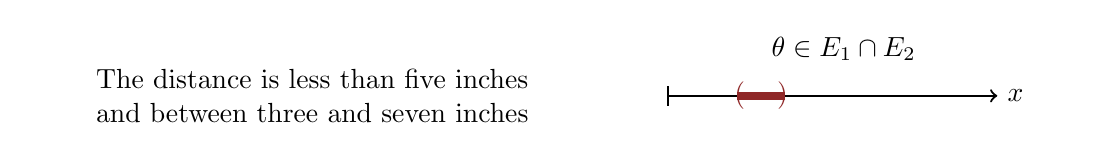
\begin{tikzpicture}[scale=0.3, thick]
  \draw[color=white] (-27, 0) to (17, 0);
  
  \node[align=center] at (-15, 0) {The distance is less than five inches\\and
                                                   between three and seven inches};
  \node[] at (7.5, 2) {$\theta \in E_{1} \cap E_{2}$};

  \draw[|->] (0, 0) -- (14,0) node[right] {$x$};
  \draw[line width=1mm, color=dark] (3, 0) node[] {$\,($} -- (5, 0) node[] {$\!)$};
\end{tikzpicture}
}
%
\subfigure[]{
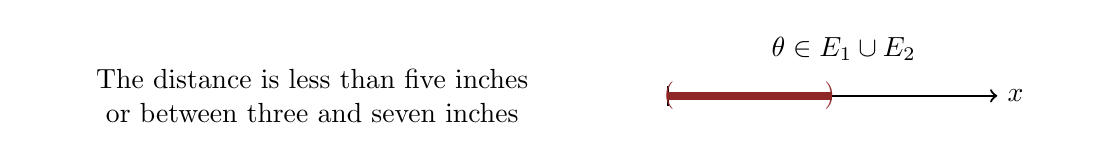
\begin{tikzpicture}[scale=0.3, thick]
  \draw[color=white] (-27, 0) to (17, 0);
   
  \node[align=center] at (-15, 0) {The distance is less than five inches\\or
                                                   between three and seven inches};
  \node[] at (7.5, 2) {$\theta \in E_{1} \cup E_{2}$};

  \draw[|->] (0, 0) -- (14, 0) node[right] {$x$};
  \draw[line width=1mm, color=dark] (0, 0) node[] {$\,($} -- (7, 0) node[] {$\!)$};
\end{tikzpicture}
}
%
\subfigure[]{
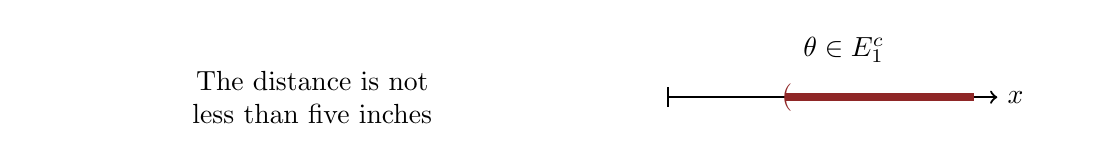
\begin{tikzpicture}[scale=0.3, thick]
  \draw[color=white] (-27, 0) to (17, 0);
   
  \node[align=center] at (-15, 0) {The distance is not\\less than five inches};
  \node[] at (7.5, 2) {$\theta \in E_{1}^{c}$};

  \draw[|->] (0, 0) -- (14, 0) node[right] {$x$};
  \draw[line width=1mm, color=dark] (5, 0) node[] {$\,($} -- (13, 0);
\end{tikzpicture}
}
\caption{(a) Systems that take continuous values, such as distances, 
can be represented with real numbers, with any logical proposition
represented by inclusion in well-behaved subsets of real numbers. 
(b) Conjuction of logical propositions is implemented with inclusion 
in set intersections, (c) disjunction with inclusion in set unions, and 
(d) negation with inclusion in set complements.}
\label{fig:real_set_logic}
\end{figure*}

\section{Equivalent Representations}

Because they map abstract systems into explicit contexts, representations
are critical to the practical implementation of logical models and their
manipulations.  Unfortunately representations also bring with them a 
dangerous subtlety -- there is no \emph{unique} representation of a 
given abstract system.

A map from one sample space into another, $s : \Theta \rightarrow \Omega$,
is \emph{measurable} if every event in $\Omega$ is generated by an event 
in $\Theta$,
%
\begin{equation*}
s^{-1} \! \left( E_{\Omega} \right) \in \EV{\Theta}.
\end{equation*}
%
Measurable maps allow us to completely generate the measurable space 
$\left( \Omega, \EV{\Omega} \right)$ by mapping forward elements of the 
initial measurable space $\left(\Theta, \EV{\Theta} \right)$; we cannot, 
however, necessarily achieve the converse as there is no guarantee that 
every event in $\EV{\Theta}$ maps to an event in $\EV{\Omega}$.
This process is also known as \emph{pushing forward} the measurable 
space $\left( \Theta, \EV{\Theta} \right)$ into the measurable space 
$\left( \Omega, \EV{\Omega} \right)$, and in this context  
$\left( \Omega, \EV{\Omega} \right)$ is denoted the \emph{pushforward} 
of $\left( \Theta, \EV{\Theta} \right)$ by $s$.

Composing a faithful representation with a measurable map,
%
\begin{equation*}
s \circ \mathfrak{e} : \mathcal{S} \rightarrow \Theta \rightarrow \Omega,
\end{equation*}
%
yields another valid representation but not necessarily a faithful one.
Because there is no guarantee that every event in $\EV{\Theta}$ maps
to an event in $\EV{\Omega}$, this pushforward may be able to represent
only a handful of propositions in the logical model.  For example,
a measurable map might round real numbers down to discrete numbers,
losing the ability to represent all but a countable number of logical 
propositions.

In order to maintain a faithful representation we need to ensure that
the events spaces are preserved by both the map and its inverse.  Here
we will say that a map $s : \Theta \rightarrow \Omega$ is 
\emph{doubly-measurable} if every event in $\EV{\Theta}$ maps to an 
event in $\EV{\Omega}$ and vice versa,
%
\begin{align*}
s \! \left( E_{\Theta} \right) &\in \EV{\Omega}
\\
s^{-1} \! \left( E_{\Omega} \right) &\in \EV{\Theta}.
\end{align*}
%
A doubly-measurable map allows us to recover either measurable space 
as a pushforward of the other, and the composition of a faithful 
representation with a doubly-measurable map,
%
\begin{equation*}
s \circ \mathfrak{e} : \mathcal{S} \rightarrow \Theta \rightarrow \Omega,
\end{equation*}
%
is then another faithful representation.  We warn the reader that there
is no conventional terminology for these maps and we have introduced
doubly-measurable here as our own terminology.

When a doubly-measurable map exists between two measurable spaces
then the two spaces can be used to specify the same logical model,
and we say that they are \emph{equivalent representations} as they provide
equivalent descriptions of a given system 
(Table \ref{tab:representation_examples}).  The set of measurable spaces
equivalent to $\left( \Theta, \EV{\Theta} \right)$ will be denoted
$\lfloor \Theta, \EV{\Theta} \rfloor$.

For example, if the sample space is discrete then we can always define 
an equivalent measurable space by simply permuting the labels.  It doesn't 
matter if we order the planets by distance from the sun, by diameter, or 
by any other metric: the measurable spaces quantify the same information 
(Figure \ref{fig:permuting_discrete_spaces}).   Similarly, we can always 
apply a transformation that warps real numbers to map between real 
sample spaces without compromising our ability to represent propositions 
with inclusion in events.  One of the most common ways this manifests in 
practice is when our descriptions require units.  The information we quantify 
doesn't depend on whether we express distance in {\aa}ngstr\"{o}ms or 
inches or meters or furlongs: each unit defines a separate but equivalent 
sample space.

\begin{figure*}
\centering
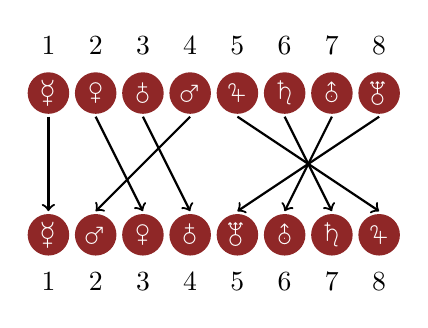
\begin{tikzpicture}[scale=0.3, thick]
  \foreach \i in {1, 2, ..., 8} {
    \node[] at ({2 * \i - 2}, 2) {$\i$};
  }  

  \fill[color=dark] (0, 0) circle (25pt) node[color=white] {$\mercury$}; 
  \fill[color=dark] (2, 0) circle (25pt) node[color=white] {$\venus$}; 
  \fill[color=dark] (4, 0) circle (25pt) node[color=white] {$\earth$}; 
  \fill[color=dark] (6, 0) circle (25pt) node[color=white] {$\mars$}; 
  \fill[color=dark] (8, 0) circle (25pt) node[color=white] {$\jupiter$}; 
  \fill[color=dark] (10, 0) circle (25pt) node[color=white] {$\saturn$}; 
  \fill[color=dark] (12, 0) circle (25pt) node[color=white] {$\uranus$}; 
  \fill[color=dark] (14, 0) circle (25pt) node[color=white] {$\neptune$};  
  
  \draw[->] (0, -1) -- (0, -5);
  \draw[->] (2, -1) -- (4, -5);
  \draw[->] (4, -1) -- (6, -5);
  \draw[->] (6, -1) -- (2, -5);
  \draw[->] (8, -1) -- (14, -5);
  \draw[->] (10, -1) -- (12, -5);
  \draw[->] (12, -1) -- (10, -5);
  \draw[->] (14, -1) -- (8, -5);
  
  \fill[color=dark] (0, -6) circle (25pt) node[color=white] {$\mercury$}; 
  \fill[color=dark] (2, -6) circle (25pt) node[color=white] {$\mars$}; 
  \fill[color=dark] (4, -6) circle (25pt) node[color=white] {$\venus$}; 
  \fill[color=dark] (6, -6) circle (25pt) node[color=white] {$\earth$}; 
  \fill[color=dark] (8, -6) circle (25pt) node[color=white] {$\neptune$};  
  \fill[color=dark] (10, -6) circle (25pt) node[color=white] {$\uranus$};
  \fill[color=dark] (12, -6) circle (25pt) node[color=white] {$\saturn$};  
  \fill[color=dark] (14, -6) circle (25pt) node[color=white] {$\jupiter$}; 

  \foreach \i in {1, 2, ..., 8} {
    \node[] at ({2 * \i - 2}, -8) {$\i$};
  }  
          
\end{tikzpicture}
\caption{Discrete sample spaces are not unique way to express a system 
as we can always permute the arbitrary labels to yield an equivalent sample 
space.  For example, we could order the planets by distance from the sun 
or diameter without affecting our ability to describe the planets themselves.}
\label{fig:permuting_discrete_spaces}
\end{figure*}

Ultimately, there are many ways to describe of a given logical model and 
measurable maps translate from one equivalent representation to another.  
Although certain representations may be more useful than others in practice, 
we have to be careful to ensure that our final analysis does not depend on 
the irrelevant details of any particular representation.

\section{Implications}

There are various Boolean operations that we can derive from the basic 
operations of negation, conjunction, and disjunction, and one of the most
powerful are \emph{implications}, which assert the truth of a statement
conditioned on the truth of another statement.  For example, we might not 
be able to assert that ``a planet has a magnetic field'' universally, but we 
might be able to assert the implication ``if a planet has a rotating core then 
it has a magnetic field''.

Implications are particularly naturally when we want to describe a target
system conditioned on the state of some other system.  Letting 
$\left(\Theta, \EV{\Theta} \right)$ be a measurable space capable of 
representing the target system and $\left(\Phi, \EV{\Phi} \right)$ be a 
measurable space capable of representing the conditioning system, an 
implication is represented as a map from points in $\Phi$ to events in 
$\EV{\Theta}$,
%
\begin{align*}
\iota_{\Theta \mid \Phi} :& \, \Phi \rightarrow \EV{\Theta}
\\
& \, \phi \mapsto \iota_{\Theta \mid \Phi} \! \left( \phi \right).
\end{align*}
%
For any event in the conditioning space, $E_{\Phi} \in \EV{\Phi}$,
the implication also defines an event in the joint sample space, 
$\Theta \times \Phi$, as the union of all of the events implied by each 
point in $E_{\Phi}$,
%
\begin{align*}
\iota^{*}_{\Theta \mid \Phi} 
&: \EV{\Phi} \rightarrow \EV{\Theta \times \Phi}
\\
& \quad \; E_{\Phi} \; \mapsto
\bigcup_{\phi \in E_{\Phi} } \iota_{\Theta \mid \Phi} \! \left( \phi \right).
\end{align*}

Because relationships are often much easier to reason about than the 
entirety of a complex system, these induced events can drastically facilitate
the description of complex systems by decomposing logical propositions 
into simpler implications.  For example, instead of having to enumerate all 
possible combinations of planetary core behavior and magnetic field, we 
can utilize the single implication that only a rotating core generates a 
magnetic field to build any logical proposition about the joint core-magnetic 
field system from a logical proposition about the core alone.  

More formally, any logical proposition representation in a joint sample space 
$\prod_{n = 1}^{N} \Theta_{n}$ can be built up sequentially, starting with an 
event in one component and adding implications one after another,
%
\begin{align*}
& E_{\Theta_{1}} \\
& \iota^{*}_{\Theta_{2} \mid \Theta_{1}} \! \left( E_{\Theta_{1}} \right) \\
& \iota^{*}_{\Theta_{3} \mid \Theta_{2}, \Theta_{1}} 
\circ
\iota^{*}_{\Theta_{2} \mid \Theta_{1}} \! \left( E_{\Theta_{1}} \right) \\
& \cdots \\
& \iota^{*}_{\Theta_{N} \mid \Theta_{N - 1}, \ldots, \Theta_{2}, \Theta_{1}}
\circ
\iota^{*}_{\Theta_{3} \mid \Theta_{2}, \Theta_{1}}  
\circ
\iota^{*}_{\Theta_{2} \mid \Theta_{1}} \! \left( E_{\Theta_{1}} \right).
\end{align*}

\chapter{Probability in Theory}

Logic provides a framework for how we can describe systems with certainty,
and the tools of probability theory allow us to assign uncertainty to logical
statements and implications.  In this section we introduce probability
distributions over first logical statements and then implications.

Unfortunately, the abstraction of probability theory means that we cannot rely 
on helpful visualizations to support the definitions and manipulations in this
section.  To use a probability distribution in any practical application, including 
visualization, we need some means of implementing them explicitly, which will 
have to wait until the next section.

\section{Probability Distributions}

When we are uncertain about our target system then we cannot
guarantee that any particular logical statement in true.  In order to
quantify uncertainty about our descriptions we assign to each event 
a \emph{probability} that quantifies how plausible it is be true.  
Probabilities themselves are bounded between 0, indicating that an 
event is absolutely false, and 1, indicating that an event is absolutely
true.

In a given expression, probabilities are designated by a 
\emph{probability distribution} which assigns probability to events,
%
\begin{equation*}
\PP : \mathcal{E} \! \left( \Theta \right) \rightarrow \left[0, 1 \right],
\end{equation*}
%
such that the probability of the null event is zero, 
$\PP \! \left[ \emptyset \right] = 0$, and the probability of the trivial
event is one, $\PP \! \left[ \Theta \right] = 1$.  These latter two conditions 
are an immediate consequence of our initial assumption that our descriptions
can be expressed by the sample space.  When using a probability distribution 
to quantify our uncertainty about a system expressed with the sample
space $\Theta$, we often write $\theta \sim \PP$ which is read as, 
``$\theta$ is distributed according to the probability distribution $\PP$''
but should really read ``Logical statements about $\Theta$ are assigned 
probabilities according to the probability distribution $\PP$''.

Probability assignments are naturally compatible with the manipulations
of logical statements.  For example, the probability of conjunctions and
disjunction are related as
%
\begin{equation*}
\PP \! \left[ E_{1} \cup E_{2} \right]
= 
\PP \! \left[ E_{1} \right] + \PP \! \left[ E_{2} \right] 
- \PP \! \left[ E_{1} \cap E_{2} \right],
\end{equation*}
%
and negations satisfy,
%
\begin{equation*}
\PP \! \left[ E \right] 
= 
\PP \! \left[ \Theta \right] - \PP \! \left[ E^{c} \right]
=
1 - \PP \! \left[ E^{c} \right].
\end{equation*}

Probability distributions also allow us to compute \emph{expectation values} 
of well-behaved functions on the sample space,
%
\begin{equation*}
\EE_{\PP} : \mathcal{F} \! \left( \Theta \right) \rightarrow \mathbb{R},
\end{equation*}
%
where $\mathcal{F} \! \left( \Theta \right)$ is the collection of well-behaved 
functions $f : \Theta \rightarrow \mathbb{R}$.  Common expectations 
include means, variances, and higher-order moments.  In fact, we
can also consider probability assignments themselves as expectations,
%
\begin{equation*}
\PP \! \left[ E \right] = \EE_{\PP} \! \left[ \mathbb{I}_{E} \right],
\end{equation*}
%
where the \emph{indicator function} of the event $E$, $\mathbb{I}_{E}$,
is defined as
%
\begin{equation*}
\mathbb{I}_{E} \! \left( \theta \right)
= 
\left\{
\begin{array}{rr}
0, & \theta \notin E \\
1, & \theta \in E
\end{array}
\right. .
\end{equation*}

The most important consequence of these definitions is that \emph{all of 
probability theory reduces to computing expectations}.  Any other operation 
that you may have encountered in probability theory can only ever be an
intermediate step in computing a final expectation.  In particular, many of 
the more non-intuitive aspects of probability theory can avoided by carefully
framing everything as an expectation -- don't try to intuit solutions, calculate 
them!

\section{Conditional Probability Distributions}

\emph{Conditional probability distributions} allow us to quantify uncertainty
about implications.  While implications assign an event to each value of the 
conditioning space, $\Phi$, a conditional probability distribution assigns a 
probability distribution to each value in the conditioning space,
%
\begin{align*}
\PP_{\Theta \mid \Phi} 
&: \EV{\Theta} \times \Phi \rightarrow \left[0, 1 \right] \\
&\quad \left( E_{\Theta}, \phi \right) \;\; \mapsto 
\PP_{\Theta \mid \Phi} \! \left[ E_{\Theta} \mid \phi \right].
\end{align*}
%
In other words, for any value of $\phi \in \Phi$ the conditional probability
distribution defines a probability distribution on $\Theta$, and for any
event in $\Theta$ the conditional probability distribution defines a 
function from $\Phi$ to probabilities.  

As with implications, conditional probability distributions can be used
to construct probability distributions on more complex spaces.  In particular,
by combining a conditional probability distribution with a probability distribution 
on the conditioning space, $\Phi$, we can construct a probability distribution 
on the joint sample space, $\Theta \times \Phi$.  This \emph{joint distribution} 
is defined implicitly by its probability assignments or expectation values.  
For example, the probability of any joint event, $E_{\Theta} \times E_{\Phi}$, 
is given by first using the conditional probability distribution to assign a probability 
to $E_{\Theta}$, $\PP_{\Theta|\Phi} \! \left[ E_{\Theta} \mid \phi \right]$, and then 
taking the expectation of this assignment over the distribution on $\Phi$,
%
\begin{equation*}
\PP_{\Theta \times \Phi} \! \left[ E_{\Theta} \times E_{\Phi} \right]
=
\mathbb{E}_{\PP_{\Phi}} \! \left[  
\PP_{\Theta|\Phi} \! \left[ E_{\Theta} \mid \phi \right] 
\cdot \mathbb{I}_{E_{\Phi}} \! \left( \phi \right)
\right],
\end{equation*}
%
where the indicator function, $\mathbb{I}_{E_{\Phi}}$, ensures that we 
take the expectation only over the event in $\Phi$.  Similarly, joint 
expectations are defined iteratively as
%
\begin{equation*}
\EE_{\PP_{\Theta \times \Phi}} \! \left[ g \! \left( \theta, \phi \right) \right]
=
\mathbb{E}_{\PP_{\Phi}} \! \left[  
\EE_{\PP_{\Theta|\Phi}} \! \Big[ 
g \! \left( \theta, \phi \right) \mid \phi 
\Big]
\right].
\end{equation*}

If we consider only the trivial event on the conditioning space $E_{\Phi} 
= \Phi$, then this construction also defines a  \emph{marginal distribution} 
on $\Theta$ by
%
\begin{align*}
\PP_{\Theta} \! \left[ E_{\Theta} \right]
&\equiv
\PP_{\Theta \times \Phi} \! \left[ E_{\Theta} \times \Phi \right] \\
&=
\mathbb{E}_{\PP_{\Phi}} \! \left[  
\PP_{\Theta|\Phi} \! \left[ E_{\Theta} \mid \phi \right]
\right],
\end{align*}
or
%
\begin{align*}
\EE_{\PP_{\Theta}} \! \left[ f \! \left( \theta \right) \right]
&\equiv
\EE_{\PP_{\Theta \times \Phi}} \! \left[ f \! \left( \theta \right) \right] \\
&=
\mathbb{E}_{\PP_{\Phi}} \! \left[  
\EE_{\PP_{\Theta|\Phi}} \! \Big[ 
f \! \left( \theta \right) \mid \phi 
\Big]
\right].
\end{align*}
%
This marginalization process allows us to collapse a joint probability 
distribution onto any of the component spaces while incorporating 
any correlations between the components.

Consequently, conditional probability distributions are powerful ways of
building probability distributions on high-dimensional spaces.  We simply 
start with a probability distribution on one low-dimensional component and 
then build up a joint distribution by adding conditional probability distributions 
for each new component,
%
\begin{align*}
& \PP_{\Theta_{1}} \\
& \PP_{\Theta_{2} \mid \Theta_{1}} \\
& \PP_{\Theta_{3} \mid \Theta_{2}, \Theta_{1}} \\
& \cdots \\
& \PP_{\Theta_{N} \mid \Theta_{N - 1}, \ldots, \Theta_{2}, \Theta_{1}}.
\end{align*}

These conditional probability distributions are often motivated by the natural 
implication structure of our target system.  In particular, if we think about 
deterministic processes as degenerate conditional probability distributions 
that assign all probability to a single event for each conditioning value,
%
\begin{equation*}
\PP_{\Theta \mid \Phi} \! \left[ E_{\Theta} \mid \phi \right]
= 
\left\{
\begin{array}{rr}
0, & E_{\Theta} \ne \hat{E} \! \left( \phi \right) \\
1, & E_{\Theta} = \hat{E} \! \left( \phi \right)
\end{array}
\right.,
\end{equation*}
%
then these conditional probability distributions can seamlessly incorporate
stochastic, deterministic, and causal relationships.  This iterative process of 
building a joint probability distribution from conditional probability distributions 
is the key building block of \emph{generative modeling}.

\section{The Invariance of Probability Distributions}

Like events, probability distributions can be defined with respect to many different 
sample spaces.  If $s : \Theta \rightarrow \Omega$ is a measurable map and 
$\PP_{\Theta}$ is a probability distribution defined over events in $\Theta$, then 
we can define an equivalent probability distribution over events in $\Omega$ by 
assigning probabilities as
%
\begin{equation*}
\PP_{\Omega} \! \left[ E_{\Omega} \right]
\equiv
\PP_{\Theta} \! \left[ s^{-1} \! \left( E_{\Omega} \right) \right].
\end{equation*}
%
Furthermore, this whole process can be inverted: if $\PP_{\Omega}$ is a probability 
distribution defined over events in $\Omega$ then we can define an equivalent 
probability distribution over events in $\Theta$ by assigning probabilities as
%
\begin{equation*}
\PP_{\Theta} \! \left[ E_{\Theta} \right]
\equiv
\PP_{\Omega} \! \left[ s \! \left( E_{\Theta} \right) \right].
\end{equation*}

Probability distributions are invariant when we move between equivalent sample 
spaces, and hence are fundamental to the underlying system and not any particular
expression of that system.  Different but equivalent sample spaces are just different 
ways to describe the same system, with events quantifying the same, invariant 
information and probability distributions quantifying the same, invariant uncertainty.

\chapter{Probability in Practice: \\Probabilistic Computation}

The immediate problem with the abstract definitions introduced in the
previous chapter is that they do not provide an explicit means of either
specifying a probability distribution, at least without considering every 
single event, or computing expectations in practical applications.  When 
the sample space is structured, however, that structure can be leveraged 
to provide the explicit implementations we need to apply probability 
theory in practice.  This is particularly evident when the sample space 
ordered, discrete, or a subset of real numbers.

\section{Cumulative Distribution Functions}

When the sample space is ordered we can completely specify a probability
distribution with only the probabilities assigned to \emph{intervals}, 
$\mathcal{I} \! \left( \Theta \right) \subset \mathcal{E} \! \left( \Theta \right)$.
Intervals are events spanning all points less than or equal to some 
distinguished point, $\theta$,
%
\begin{equation*}
I \! \left( \theta \right) = \left\{ \theta' \in \Theta \mid \theta' \leq \theta \right\}.
\end{equation*}
%
The function that assigns these probabilities,
%
\begin{align*}
P 
&: \Theta \rightarrow \mathcal{I} \! 
\left( \Theta \right) \rightarrow \left[0, 1 \right]
\\
&\quad \theta \mapsto 
I \! \left( \theta \right) \;\; \mapsto 
\PP \! \left[ I \! \left( \theta \right) \right].
\end{align*}
%
is called the \emph{cumulative distribution function}.  

Cumulative distribution functions naturally pushforward from one 
sample space into another.  Given a measureable map 
$s : \Theta \rightarrow \Omega$, the cumulative distribution function
on $\Omega$ is defined by
%
\begin{equation*}
P_{\Omega} \! \left( I_{\omega} \right) 
\equiv 
P_{\Theta} \! \left( s^{-1} \! \left( I_{\omega} \right) \right).
\end{equation*}

\section{Implementations of Probability Distributions \\ 
over Discrete Sample Spaces}

Every discrete sample space features a natural measure which we 
can use to not only specify all other measures, and hence probability 
distributions, but also convert expectations into summations.

\subsection{The Counting Measure and Mass Functions}

The \emph{counting measure} on a discrete space assigns unit
measure to the \emph{point events},
%
\begin{equation*}
\chi \! \left( \theta \right) = 1, \, \forall \theta \in \Theta.
\end{equation*}
%
In order to compute the measure of any other event we 
simply count the elements in that event,
%
\begin{equation*}
\chi \! \left( E \right)
=
\sum_{\theta \in E}  1 = \left| E \right|,
\end{equation*}
%
hence the name.  Similarly, Lebesgue integrals reduce to a 
summation over the sample space weighted by the function 
values,
%
\begin{equation*}
\mathcal{I}_{\chi} \! \left[ f \right]
=
\sum_{\theta \in \Theta} 
f \! \left( \theta \right) \chi \! \left( \theta \right)
=
\sum_{\theta \in \Theta} f \! \left( \theta \right),
\end{equation*}
%
for any $f \in \mathcal{F} \! \left( \Theta \right)$.

Because the counting measure assigns zero measure only to the
null event, all discrete measures are absolutely continuous with
respect to it.  Consequently, any discrete measure can be defined
by its Radon-Nikodym derivative with respect to the counting measure.
In this case the Radon-Nikodym derivative is denoted a 
\emph{mass function}
%
\begin{equation*}
m : \Theta \rightarrow \RR^{+}.
\end{equation*}
%
Measures and Lebesgue integrals then reduce to discrete summations
weighted by the mass function,
%
\begin{align*}
\mu \! \left( E \right)
&=
\sum_{\theta \in E} m \! \left( \theta \right)
\\
\mathcal{I}_{\mu} \! \left[ f \right]
&=
\sum_{\theta \in \Theta} f \! \left( \theta \right) m \! \left( \theta \right).
\end{align*}

Moreover, the Radon-Nikodym derivative between different discrete 
measures reduces to the simple ratio of their mass functions,
%
\begin{equation*}
\frac{ \dd \mu_{2} }{ \dd \mu_{1} } \! \left( \theta \right)
=
\frac{ m_{2} \! \left( \theta \right) }{ m_{1} \! \left( \theta \right) }.
\end{equation*}

\subsection{Transforming Counting Measures and Mass Functions}

The counting measure, and hence mass functions, also have the
convenient property that they transform naturally with changes to
the underlying sample space.  Given a measurable map 
$s : \Theta \rightarrow \Omega$, a mass function on $\Theta$
pushes forward to a mass function on $\Omega$,
%
\begin{equation*}
m_{\Omega} \! \left( \omega \right) 
\equiv 
m_{\Theta} \! \left( s^{-1} \! \left( \omega \right) \right).
\end{equation*}

\subsection{Probability Mass Functions}

Mass functions corresponding to probability distributions reduce
to \emph{probability mass functions}, which assigns probability to the
point events,
%
\begin{equation*}
p : \Theta \rightarrow \left[0, 1\right].
\end{equation*}
%
such that
%
\begin{equation*}
1 = \pi \! \left[ \Theta \right] = \sum_{\theta \in \Theta} p \! \left( \theta \right).
\end{equation*}

\subsection{Conditional Probability Mass Functions}

Probability mass functions immediately generalize to specify conditional 
probability distributions by simply adding a conditioning variable,
%
\begin{equation*}
p_{\Theta \mid \Phi} : \Theta \times \Phi \rightarrow \left[0, 1\right].
\end{equation*}
%
Conditional probabilities and conditional expectations are computed
as above,
%
\begin{align*}
\PP_{\Theta \mid \Phi}  \! \left[ E \mid \phi \right]
&=
\sum_{\theta \in E} p_{\Theta \mid \Phi}  \! \left( \theta \mid \phi \right),
\\
\mathbb{E}_{\PP_{\Theta \mid \Phi} } \! \left[ f \mid \phi \right]
&=
\sum_{\theta \in \Theta} f \! \left( \theta \right) 
p_{\Theta \mid \Phi}  \! \left( \theta \mid \phi \right),
\end{align*}

A huge advantage of this representation is that it drastically simplifies the
construction of joint and marginal probability distributions.  Instead of 
implicitly defining an abstract joint distribution with probability assignments
or expectations, for example, we can construct an explicit joint probability 
mass function as the product of a conditional mass function and a marginal 
mass function,
%
\begin{equation*}
p_{\Theta \times \Phi} \! \left( \theta, \phi \right) = 
p_{\Theta \mid \Phi} \! \left( \theta | \phi \right) p_{\Phi} \! \left( \phi \right),
\end{equation*}
%
which readily gives joint probabilities and joint expectations.

Marginalization proceeds similarly -- the marginal probability mass function
is given by simply summing the joint probability mass function over the
nuisance components,
%
\begin{align*}
p_{\Theta} \! \left( \theta \right)
&= 
\sum_{\phi \in \Phi}  p_{\Theta \times \Phi} \! \left( \theta, \phi \right) \\
&=
\sum_{\phi \in \Phi}
p_{\Theta \mid \Phi} \! \left( \theta | \phi \right) p_{\Phi} \! \left( \phi \right).
\end{align*}

Bayes' Theorem implies that any decomposition of a joint probability
mass function is equal,
%
\begin{equation} \label{eqn:discrete_bayes}
p_{\Phi \mid \Theta} \! \left( \phi | \theta \right) p_{\Theta} \! \left( \theta \right)
=
p_{\Theta \times \Phi} \! \left( \theta, \phi \right) 
= 
p_{\Theta \mid \Phi} \! \left( \theta | \phi \right) p_{\Phi} \! \left( \phi \right),
\end{equation}
%
and from this one equality we can then recover the various implications of
Bayes' Theorem.  For example,
%
\begin{equation*}
\pi_{\Theta \mid \Phi} =
\frac{ \dd \pi_{\Phi \mid \Theta} }{ \dd \pi_{\Phi} }
\pi_{\Theta}
\end{equation*}
%
becomes
%
\begin{equation*}
p_{\Theta \mid \Phi} \! \left( \theta \mid \phi \right) =
\frac{ p_{\Phi \mid \Theta} \! \left( \phi \mid \theta \right) }
{ p_{\Phi} \! \left( \phi \right) }
p_{\Theta} \! \left( \theta \right),
\end{equation*}
%
which is an immediate consequence of dividing both sides of the joint
equality \eqref{eqn:discrete_bayes} by $p_{\Phi} \! \left( \phi \right)$.

\subsection{Relating Probability Mass Functions and Cumulative 
Distribution Functions}

Because probability mass functions and cumulative distribution functions 
both specify the same probability distribution, one can always be used to 
construct the other.  Given a probability mass function, for example, we 
can construct the cumulative distribution function as
%
\begin{equation*}
P \! \left( \theta \right)
= \PP \! \left[ I \! \left( \theta \right) \right]
= \sum_{\theta' \in I ( \theta )} p \! \left( \theta' \right).
\end{equation*}
%
Similarly, we can construct a probability mass function from a cumulative
distribution function as
%
\begin{equation*}
p \! \left( \theta \right) = 
P \! \left( \theta \right)
- P \! \left( \theta_{-} \right),
\end{equation*}
%
where $\theta_{-}$ is the largest element of $\Theta$ less that $\theta$,
%
\begin{equation*}
\theta_{-} = \max \left\{ \theta' \in \Theta \mid \theta' < \theta \right\}.
\end{equation*}

\section{Implementations of Probability Distributions over Real
Numbers}

When the sample space are $D$-dimensional real numbers, or
a subset thereof, there are always an uncountably infinite number 
of point events and we can't assign a finite measure to each without
the measure of any dense event becoming infinite.  Consequently,
the counting measure becomes pathological, assigning either infinite 
measure or zero measure to every dense event.  Fortunately, the real 
numbers admit their own natural measure on which we can implement 
probability distributions in practice.

\subsection{The Lebesgue Measure and Density Functions}

\textbf{Lebesgue measure on R assigns measure based on interval
length, then generalize as a product of Lebesgue measures that
assigns measure based on volume.}

The Lebesgue measure on the one-dimensional real numbers
assigns to each interval,
%
\begin{equation*}
I = \left[a, b \right] \subset \RR,
\end{equation*}
%
a measure proportional to its length,
%
\begin{equation*}
\lambda \! \left( I \right) = b - a.  
\end{equation*}

This generalizes to the general Lebesgue measure, $\lambda$, 
which assigns to each rectangular neighborhood
%
\begin{equation*}
I_{D} = \prod_{d=1}^{D} I_{d} = \prod_{d=1}^{D} \left[a_{d}, b_{d} \right]
\subset \RR^{D},
\end{equation*}
%
a measure proportional to its volume,
%
\begin{equation*}
\lambda \! \left( I_{d} \right) = 
\prod_{d = 1}^{D} \left(b_{d} - a_{d} \right).  
\end{equation*}
%
Although not immediately obvious, this condition implies that the 
Lebesgue measure of an arbitrary event is also given by the
enclosed volume specified by the Riemann integral over that event
%
\begin{equation*}
\lambda \! \left( E \right)= \int_{E} \dd^{D} \theta.
\end{equation*}
%
Because of this equivalence, it is common shorthand to write the 
Lebesgue measure on $\Theta = R^{D}$ as 
%
\begin{equation*}
\lambda = \dd^{D} \theta = \prod_{d = 1}^{D} \dd \theta_{d}.
\end{equation*}

Similarly, Lebesgue integrals with respect to the Lebesgue measure
(mathematicians have sick sense of humor) also reduce to Riemann
integrals,
%
\begin{equation*}
\mathcal{I}_{\lambda} \! \left( f \right)
= \int_{\Theta} f \! \left( \theta \right) \dd \theta.
\end{equation*}
%
An immediate consequence of this result is that all point events
have zero Lebesgue measure.

Provided that a measure does not assign non-zero measure to any
point events, it will be absolutely continuous with respect to the
Lebesgue measure and hence can be completely specified with
the corresponding Radon-Nikodym derivative.  In this case the
Radon-Nikodym derivative is denoted a \emph{density function},
%
\begin{equation*}
m : \Theta \rightarrow \RR^{+}.
\end{equation*}
%
As above, any measure or Lebesgue integral becomes a standard
Riemann integral that can be readily computed with the usual
calculus techniques,
%
\begin{align*}
\mu \! \left( E \right)
&=
\mathcal{I}_{\lambda} \! \left[ m \cdot I_{E} \right]
=
\int_{E} m \! \left( \theta \right) \dd \theta
\\
\mathcal{I}_{\mu} \! \left[ f \right]
&=
\mathcal{I}_{\lambda} \! \left[ f \cdot m \right]
=
\int_{\Theta} f \! \left( \theta \right) m \! \left( \theta \right) \dd \theta.
\end{align*}

The Radon-Nikodym derivative between two different real measures
behaves exactly as in the discrete case.  If $\mu_{2}$ is
absolutely continuous with respect to $\mu_{1}$ then the density
$m_{2} \! \left( \theta \right)$ can vanish only when the density
$m_{1} \! \left( \theta \right)$ vanishes, and the corresponding 
Radon-Nikodym derivative is given by
%
\begin{equation*}
\frac{ \dd \mu_{2} }{ \dd \mu_{1} } \! \left( \theta \right)
=
\frac{ m_{2} \! \left( \theta \right) }{ m_{1} \! \left( \theta \right) }.
\end{equation*}
%
When both densities vanish we have to be careful take an
appropriate limit in order to evaluate the Radon-Nikodym derivative.

\subsection{Transforming Lebesgue Measures and Density Functions}

One of the most subtle properties of Lebesgue measures, and
hence density functions, is that they do not transform as naturally
as their discrete counterparts.  The difficulty is that nonlinear
transformations warp the real numbers, distorting volumes and,
consequently, the Lebesgue measure.  

Consider a nonlinear, measurable map $s : \Theta \rightarrow \Omega$,
and let $\tilde{\lambda}_{\Omega}$ be the corresponding pushforward 
of the Lebesgue measure on $\Theta$ onto $\Omega$,
%
\begin{equation*}
\tilde{\lambda}_{\Omega} \! \left( E_{\Omega} \right)
\equiv
s_{*} \lambda_{\Theta} \! \left( E_{\Omega} \right)
=
\mu^{L}_{\Theta} \! \left[ s^{-1} \! \left( E_{\Omega} \right) \right].
\end{equation*}
%
The pushforward $\tilde{\lambda}_{\Omega}$ is not the Lebesgue 
measure on $\Omega$, rather the two are related by the Radon-Nikodym
derivative
%
\begin{equation*}
\frac{ \dd \lambda_{\Omega} }
{\dd \tilde{\lambda}_{\Omega} }
=
\left| \mathbf{J} \right|,
\end{equation*}
%
where the matrix
%
\begin{equation*}
J_{ij} 
= 
\frac{\partial \omega_{i} }{ \partial \theta_{j} }
\equiv 
\frac{ \partial s_{i} }{ \partial \theta_{j} }
\end{equation*} 
%
is called the \emph{Jacobian} of the transformation.  The determinant
of the Jacobian matrix quantifies how the nonlinear transformation 
warps volumes and hence the Lebesgue measure.

This nontrivial relationship between Lebesgue measures and their
pushforwards has an important consequence for density functions.  
Density functions do not transform as we might naively expect,
%
\begin{equation*}
m_{\Omega} \! \left( \omega \right) 
\ne 
m_{\Theta} \! \left( s^{-1} \! \left( \omega \right) \right),
\end{equation*}
%
rather they too are modified by the determinant of the Jacobian matrix,
%
\begin{equation*}
m_{\Omega} \! \left( \omega \right) 
= 
m_{\Theta} \! \left( s^{-1} \! \left( \omega \right) \right) | \mathbf{J} |^{-1}.
\end{equation*}
%
We can also motivate this relationship by considering the invariance
of Lebesgue integrals.  Equivalent sample spaces feature distinct
Lebesgue measure and density functions, but they must have the
\emph{same Lebesgue integrals} (Figure \ref{fig:pdf_transform}).
The Lebesgue integrals are invariant only if the Lebesgue measures
and densities transform oppositely to each other.

\begin{figure*}
\centering
%
\subfigure[]{
%\begin{tikzpicture}[scale=0.3, thick, show background rectangle]
\begin{tikzpicture}[scale=0.3, thick]
  \node[] at (0,0) {
\includegraphics[width=5cm]{density.eps}};
  \foreach \i in {-10.5, -10, ..., 10.5} {
    \draw[-, color=gray80] (-11, \i) to (11, \i);
    \draw[-, color=gray80] (\i, -11) to (\i, 11);
  }  
  \node[] at (0,0) {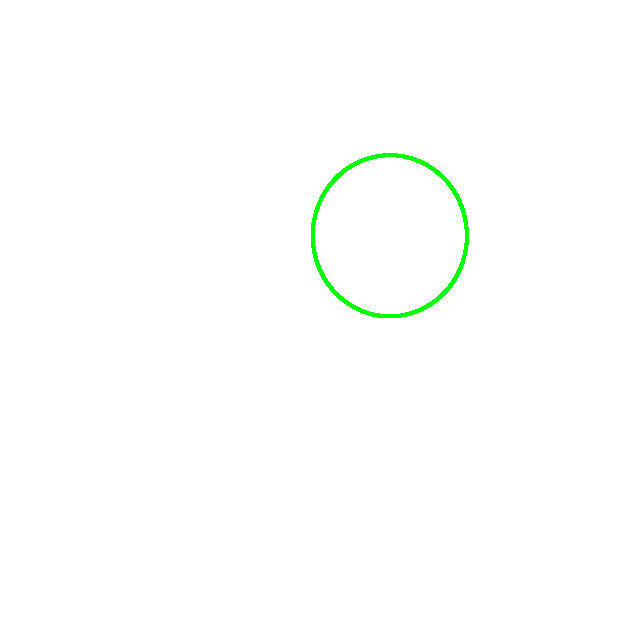
\includegraphics[width=5cm]{area.eps}};
  \node[] at (0, -13) { $\mu \! \left( E_{\Theta} \right) = \int_{E_{\Theta}} 
                                   m_{\Theta} (\theta_{1}, \theta_{2}) 
                                   \dd \theta_{1} \dd \theta_{2} $ };
\end{tikzpicture}
}
%
\subfigure[]{
%\begin{tikzpicture}[scale=0.3, thick, show background rectangle]
\begin{tikzpicture}[scale=0.3, thick]
  \node[] at (0,0) {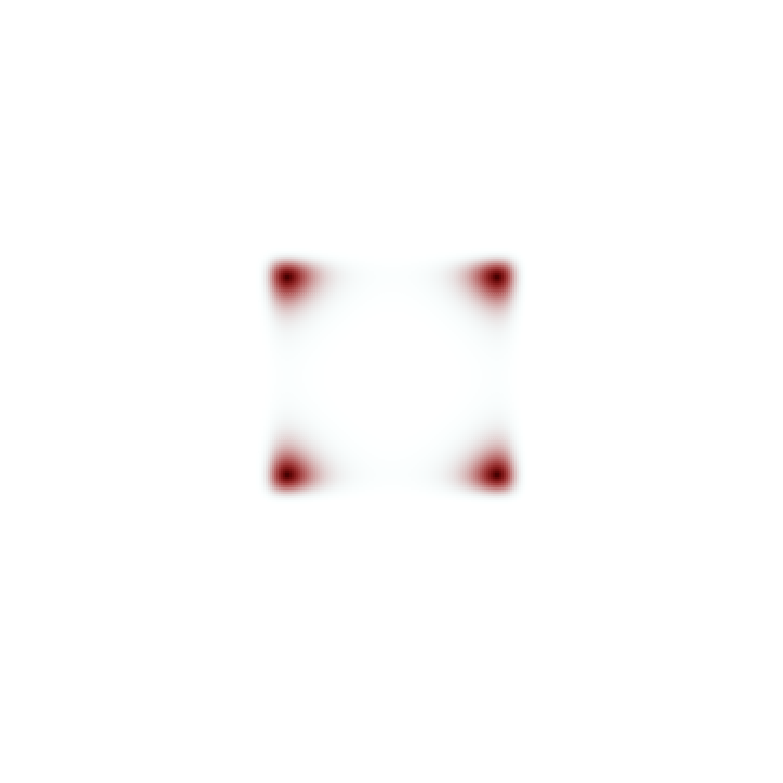
\includegraphics[width=5cm]{transformed_density.eps}};
  \foreach \i in {-10.9969, -10.9428, -10.8857, -10.8251, -10.7605, -10.6915, -10.6174, 
                        -10.5374, -10.4504, -10.355, -10.2497, -10.1319, -9.99835, -9.84419, 
                        -9.66186, -9.4387, -9.15099, -8.74547, -8.05217, 0., 8.05217, 
                        8.74547, 9.15099, 9.4387, 9.66186, 9.84419, 9.99835, 10.1319, 
                        10.2497, 10.355, 10.4504, 10.5374, 10.6174, 10.6915, 10.7605,
                        10.8251, 10.8857, 10.9428, 10.9969} {
    \draw[-, color=gray80] (-11, \i) to (11, \i);
    \draw[-, color=gray80] (\i, -11) to (\i, 11);
  }  
  \node[] at (0,0) {
\includegraphics[width=5cm]{transformed_area.eps}};
  \node[] at (0, -13) { $\mu \! \left( s \! \left( E_{\Theta} \right) \right)
                                   = \int_{s(E_{\Theta})} 
                                   m_{\Omega} (\omega_{1}, \omega_{2}) 
                                   \dd \omega_{1} \dd \omega_{2}$ };
\end{tikzpicture}
}
\caption{When sample spaces are real, each sample space has
its own density functions (red), events (green), and differential volumes 
(grey).  Here the sample space in (b) is related to the sample space in 
(a) by the compatible mapping $\left(\omega_{1}, \omega_{2} \right) 
= s \!\left( \theta_{1}, \theta_{2} \right)$. All of these differences, however, 
exactly compensate to ensure that integrals always yield the same 
measures, $\mu \! \left( E_{\Theta} \right) = 
\mu \! \left( s \! \left( E_{\Theta} \right) \right) $.
}
\label{fig:pdf_transform}
\end{figure*}

Consequently, density functions depend not just on the abstract
system that we're trying to describe but also on the particular 
representation that we're using.  The only application of density
functions that are not sensitive to this dependence is integration,
and we have to be careful not to take densities too seriously when
they are not explicitly under an integral sign.

\subsubsection{Univariate Examples of Density Transformations}

A common motivation for transforming the sample space, and
hence any probability density functions, is when the nominal sample
space is contained.  Mapping to an unconstrained sample space
removes the unconstraint, potentially simplifying calculations.

For example, let $p_{\Theta} \! \left( \theta \right)$ be a probability 
distribution function defined on $\Theta = \RR^{+}$.  We can 
unconstrained the positivity constraint by applying a logarithmic 
transformation,
%
\begin{equation*}
\omega = s \! \left( \theta \right) = \log \theta \in \RR.
\end{equation*}
%
which results in the Jacobian
%
\begin{equation*}
J 
= \frac{ \partial s }{ \partial \theta} \! \left( \omega \right) 
= \frac{1}{\exp \! \left( \omega \right)}
\end{equation*}
%
and the transformed probability density function on $\Omega = \RR$,
%
\begin{align*}
p_{\Omega} \! \left( \omega \right)
&=
p_{\Theta} \! \left( s^{-1} \! \left( \omega \right) \right) \left|J\right|^{-1}
\\
&=
p_{\Theta} \! \left( s^{-1} \! \left( \omega \right) \right)
\exp \! \left( \omega \right).
\end{align*}

Similarly, we can unconstrain a sample space representing probabilities
themselves, $\Theta = \left[0, 1 \right]$ by applying a logistic transform,
%
\begin{equation*}
\omega = s \! \left( \theta \right) = \frac{1}{1 + \exp( - \theta ) } \in \RR.
\end{equation*}
%
This results in the Jacobian
%
\begin{equation*}
J 
= \frac{ \partial s }{ \partial \theta} \! \left( \omega \right) 
= \frac{1}{\omega \! \left( 1 - \omega \right) }
\end{equation*}
%
and the transformed probability density function on $\Omega = \RR$,
%
\begin{align*}
p_{\Omega} \! \left( \omega \right)
&=
p_{\Theta} \! \left( s^{-1} \! \left( \omega \right) \right) \left|J\right|^{-1}
\\
&=
p_{\Theta} \! \left( s^{-1} \! \left( \omega \right) \right)
\omega \! \left( 1 - \omega \right).
\end{align*}

\subsubsection{A Multivariate Example of Density Transformations}

To see how much a probability density function can be warped, consider 
a two-dimensional sample space with real components 
$\left( \theta_{1}, \theta_{2} \right)$ and the probability density function
%
\begin{equation*}
p_{\Theta} \! \left( \theta_{1}, \theta_{2} \right)
\propto
\exp \! \left( - \frac{\theta_{1}^{2} + \theta_{2}^{2}}{2} \right).
\end{equation*}
%
and the measurable map
%
\begin{equation*}
\left( \omega_{1}, \omega_{2} \right) 
= 
r \! \left( \theta_{1}, \theta_{2} \right) 
= 
\left( s \! \left( \theta_{1} \right), s \! \left( \theta_{2} \right) \right),
\end{equation*}
%
where the component maps are given by
%
\begin{equation*}
s \! \left( \theta \right)
=
\log \! \left(
\frac{ \pi + 2 \, \mathrm{atan} \! \left( \alpha \, \theta \right) }
{ \pi - 2 \, \mathrm{atan} \! \left( \alpha \, \theta \right) }
\right)
\end{equation*}
%
with the inverse
%
\begin{equation*}
s^{-1} \! \left( \omega \right)
=
\frac{1}{\alpha} 
\tan \! \left(
\frac{\pi}{2} \, \frac{e^{\omega} - 1}{e^{\omega} + 1} \right)
\end{equation*}
%
and Jacobian
%
\begin{equation*}
J \! \left( \omega \right)
=
\frac{ \partial s }{ \partial \theta } \! \left( \omega \right)
=
\frac{\alpha}{\pi} \frac{ \left( 1 + e^{\omega} \right)^{2} }{ e^{\omega} }
\sin^{2} \! \left( \frac{ \pi }{ 1 + e^{\omega} } \right).
\end{equation*}
%
The Jacobian of the complete map is then given by
%
\begin{equation*}
\mathbf{J} = 
\begin{bmatrix}
J & 0 \\
0 & J
\end{bmatrix},
\end{equation*}
%
with the determinant $| \mathbf{J} | = J^{2}$.  Hence the transformed
probability density function and differential volume are given by
%
\begin{equation*}
p_{\Omega} \! \left( \omega_{1}, \omega_{2} \right)
=
p_{\Theta} \! \left( 
s^{-1} \! \left( \omega_{1} \right), 
s^{-1} \! \left( \omega_{2} \right) \right)
J^{-2} \! \left( \omega \right)
\end{equation*}
%
and
%
\begin{equation*}
\dd \omega_{1} \dd \omega_{2}
=
J^{2} \dd \theta_{1} \dd \theta_{2},
\end{equation*}
%
respectively.  The extreme differences between these two representations
are evident graphically in Figure \ref{fig:pdf_transform}.

\subsection{Probability Density Functions}

Density functions corresponding to probability distributions reduce
to \emph{probability density function} which assign a positive value 
to each point in the sample space,
%
\begin{equation*}
p : \Theta \rightarrow \mathbb{R}^{+}.
\end{equation*}
such that
%
\begin{equation*}
1 = \pi \! \left( \Theta \right) = \int_{\Theta} p \! \left( \theta \right) \dd \theta.
\end{equation*}
%
These values, known as \emph{probability densities}, have no particular 
meaning of their own and instead exist only to be integrated to give 
probabilities,
%
\begin{equation*}
\pi \! \left( E \right)
=
\int_{E} p \! \left( \theta \right) \dd \theta,
\end{equation*}
%
and expectations,
%
\begin{equation*}
\mathbb{E}_{\pi} \! \left[ f \right]
=
\int_{\Theta} f \! \left( \theta \right) p \! \left( \theta \right) \dd \theta.
\end{equation*}

This is an important point that is worth repeating -- probability densities 
are meaningless until they have been integrated over some event.  To 
analogize with physics, the event over which we integrate corresponds 
to a \emph{volume} and the probability given by integrating the density 
over such a volume corresponds to a \emph{mass}.  When we want to 
be careful to differentiate between probabilities and probability densities 
we'll use \emph{probability mass} to refer to the former.

\subsection{Conditional Probability Density Functions}

Just as in the discrete case, probability density functions can be 
immediately extended to implement conditional probability distributions 
by simply adding a conditioning variable,
%
\begin{equation*}
p_{\Theta \mid \Phi} : \Theta \times \Phi \rightarrow \mathbb{R}^{+},
\end{equation*}
%
with conditional probabilities and conditional expectations reducing
to integrals,
%
\begin{align*}
\pi_{\Theta \mid \Phi}  \! \left( E \mid \phi \right)
&=
\int_{E} p_{\Theta \mid \Phi}  \! \left( \theta \mid \phi \right) \dd \theta,
\\
\mathbb{E}_{\pi_{\Theta \mid \Phi} } \! \left[ f \mid \phi \right]
&=
\int_{\Theta} f \! \left( \theta \right) 
p_{\Theta \mid \Phi}  \! \left( \theta \mid \phi \right) \dd \theta,
\end{align*}

Likewise, probability density functions representing joint and marginal 
probability distributions are easy to construct for conditional probability 
density functions.  Joint probability density functions are given by a simple
multiplication,
%
\begin{equation*}
p_{\Theta \times \Phi} \! \left( \theta, \phi \right) = 
p_{\Theta \mid \Phi} \! \left( \theta | \phi \right) p_{\Phi} \! \left( \phi \right),
\end{equation*}
%
and marginal probability density functions are given by integrating out the
nuisance components,
%
\begin{align*}
p_{\Theta} \! \left( \theta \right)
&= 
\int_{\Phi} p_{\Theta \times \Phi} \! \left( \theta, \phi \right) \dd \phi \\
&=
\int_{\Phi}
p_{\Theta \mid \Phi} \! \left( \theta | \phi \right) 
p_{\Phi} \! \left( \phi \right) \dd \phi.
\end{align*}

Bayes' Theorem also implies that any decomposition of a joint probability
density function is equal,
%
\begin{equation} \label{eqn:real_bayes}
p_{\Phi \mid \Theta} \! \left( \phi | \theta \right) p_{\Theta} \! \left( \theta \right)
=
p_{\Theta \times \Phi} \! \left( \theta, \phi \right) 
= 
p_{\Theta \mid \Phi} \! \left( \theta | \phi \right) p_{\Phi} \! \left( \phi \right),
\end{equation}
%
and from this one equality we can then recover the various implications of
Bayes' Theorem.  For example,
%
\begin{equation*}
\pi_{\Theta \mid \Phi} =
\frac{ \dd \pi_{\Phi \mid \Theta} }{ \dd \pi_{\Phi} }
\pi_{\Theta}
\end{equation*}
%
becomes
%
\begin{equation*}
p_{\Theta \mid \Phi} \! \left( \theta \mid \phi \right) =
\frac{ p_{\Phi \mid \Theta} \! \left( \phi \mid \theta \right) }
{ p_{\Phi} \! \left( \phi \right) }
p_{\Theta} \! \left( \theta \right),
\end{equation*}
%
which is an immediate consequence of dividing both sides of the joint
equality \eqref{eqn:real_bayes} by $p_{\Phi} \! \left( \phi \right)$.

\subsection{Relating Probability Density Functions and Cumulative 
Distribution Functions}

As with their discrete counterparts, probability density functions 
and cumulative distribution functions can always be derived from
each other because they specify the same probability distribution.  
Cumulative distribution functions, for example, are given by 
integrating over probability density functions,
%
\begin{equation*}
P \! \left( \theta \right)
= \pi \! \left[ I \! \left( \theta \right) \right]
= \int_{\theta_{\min}}^{\theta} p \! \left( \theta' \right) \dd \theta.
\end{equation*}

Probability density functions, on the other hand, are given by 
differentiating cumulative distribution functions,
%
\begin{equation*}
p \! \left( \theta \right) = 
\frac{\partial P \! \left( \theta \right) }{ \partial \theta}.
\end{equation*}
%
Note that if we map to an equivalent measurable space with 
$s : \Theta \rightarrow \Omega$, then the derivative
acquires a factor of the inverse Jacobian so that the
corresponding probability density function transforms
as necessary,
%
\begin{equation*}
p \! \left( \omega \right) 
= 
\frac{\partial P \! \left( \omega \right) }{ \partial \omega}
=
\frac{\partial P \! \left( s^{-1} \! \left( \omega \right) \right) }
{ \partial \theta}
\frac{ \partial \theta }{ \partial \omega }
= 
p \! \left( s^{-1} \! \left( \omega \right) \right) \left| \mathbf{J}^{-1} \right|.
\end{equation*}

\subsection{Implementations of Mixed Probability Distributions}

Distributions over samples spaces that have both a discrete, $\Phi$,
and a real $\Psi$, component can be implemented by leveraging 
discrete and continuous representations of conditional distributions.  

For example, a distribution over $\Theta = \Phi \times \Psi$ can be
specified by conditioning the discrete component with the real
component, $\pi_{\Phi \mid \Psi}$, and providing a marginal distribution
over the real component, $\pi_{\Psi}$.  Using a conditional
probability mass function for the former and a probability density function
for the latter, the probability of any event is given by
%
\begin{align*}
\pi_{\Theta} \! \left( E \right)
&=
\pi_{\Theta} \! \left( E_{\Phi} \times E_{\Psi} \right)
\\
&=
\EE_{\pi_{\Psi}} \! \left[
\pi_{\Phi \mid \Psi} \! \left(  E_{\Phi} \mid \psi \right)
\cdot
\mathbb{I}_{E_{\Psi}} \! \left( \psi \right)
\right] 
\\
&= 
\int_{E_{\Psi} }
\sum_{\phi \in E_{\Phi} } p_{\Phi \mid \Psi} \! \left( \phi \mid \psi \right)
p_{\Psi} \! \left( \psi \right) \dd \psi,
\end{align*}
%
with expectations given similarly by
%
\begin{align*}
\EE_{\pi_{\Theta}} \! \left[ f \right]
&=
\EE_{\pi_{\Psi}} \! \left[
\EE_{\pi_{\Phi \mid \Psi}} \! \left[  f \mid \psi \right]
\right] 
\\
&= 
\int_{E_{\Psi} } \sum_{\phi \in E_{\Phi} } f \! \left( \phi, \psi \right) 
p_{\Phi \mid \Psi} \! \left( \phi \mid \psi \right)
p_{\Psi} \! \left( \psi \right) \dd \psi.
\end{align*}

Equivalently, we could also condition the real component on the
discrete component, $\pi_{\Psi \mid \Phi}$ and provide a marginal 
distribution over the discrete component, $\pi_{\Phi}$.  We could 
then represent the distribution with a conditional probability density 
function for the former and a probability mass function for the latter.  
Likewise, the probability of any event is given by
%
\begin{align*}
\pi_{\Theta} \! \left( E \right)
&=
\pi_{\Theta} \! \left( E_{\Phi} \times E_{\Psi} \right)
\\
&=
\EE_{\pi_{\Phi}} \! \left[
\pi_{\Psi \mid \Phi} \! \left(  E_{\Psi} \mid \phi \right)
\cdot
\mathbb{I}_{E_{\Phi}} \! \left( \phi \right)
\right] 
\\
&= 
\sum_{\phi \in E_{\Phi} } \int_{E_{\Psi} }
p_{\Psi \mid \Phi} \! \left( \psi \mid \phi \right) 
p_{\Phi} \! \left( \phi \right) \dd \psi,
\end{align*}
%
with expectations given similarly by
%
\begin{align*}
\EE_{\PP_{\Theta}} \! \left[ f \right]
&=
\EE_{\PP_{\Phi}} \! \left[
\EE_{\PP_{\Psi \mid \Phi}} \! \left[  f \mid \phi \right]
\right] 
\\
&= 
\sum_{\phi \in E_{\Phi} } \int_{E_{\Psi} }
f \! \left( \phi, \psi \right) 
p_{\Psi \mid \Phi} \! \left( \psi \mid \phi \right)
p_{\Phi} \! \left( \phi \right) \dd \psi.
\end{align*}

Regardless of how we choose to decompose the mixed distribution,
combining probability density functions and probability mass functions
makes specifying and manipulating these distributions straightforward in
practice.

\section{Stochastic Implementations of Probability Distributions}

We can also specify any probability distributions and compute its
expectations \emph{stochastically}.  A \emph{stochastic process} is 
any mechanism that generates a sequence of states, or \emph{samples},
from a given sample space, 
$\left\{ \theta_{1}, \ldots, \theta_{N} \right\} \subset \Theta$.  In general,
the generation of the $n$-th state in the sequence, $\theta_{n}$, can
depend on all previous states in the sequence, 
$\left\{ \theta_{1}, \ldots, \theta_{n - 1} \right\}$.

A stochastic process implements a given probability distribution if 
the samples themselves can be used to recover all expectations as 
the size of the sequence becomes infinitely large. More formally, if
%
\begin{equation*}
\lim_{N \rightarrow \infty} \frac{1}{N} 
\sum_{n = 1}^{N} f \! \left( \theta_{n} \right)
= \EE_{\pi} \! \left[ f \right],
\end{equation*}
%
for all well-behaved functions, $f : \Theta \rightarrow \RR$, then the 
stochastic process implements all computations with respect to the 
probability distribution $\pi$.

This procedure, and hence the resulting samples, are \emph{exact} 
if every state in the sequence is generated independently of any previous 
states.  In other words, samples are exact when the stochastic process 
generates samples one at a time, with no dependence on the preceding 
or following samples.  If samples are not exact we refer to them as 
\emph{correlated}.

Exact stochastic processes are, by construction, perfectly
\emph{random} processes: there is no way to predict any element 
of the sampling sequence given the state of other samples in
that sequence.  Unfortunately such randomness is impossible to 
achieve in practice as computers are fundamentally deterministic.
Instead we rely on \emph{pseudorandom} processes which
generate sequences in a convoluted but ultimately deterministic
fashion.  When we are ignorant of the precise configuration of a
pseudorandom process the resulting samples \emph{appear} to be
random for all intents and purposes.

Pseudorandom processes that target specific probability distributions, 
or \emph{pseudorandom number generators}, can be devised for 
many simple probability distributions.  Unfortunately they are typically 
impossible to construct for the more complex distributions that are
often of practical interest.
\chapter{Probability in Practice: The Complexity of Computation}

The beauty of probability theory is that, once we have selected a
\emph{target} probability distribution, the only well-posed computations
are expectations.  As noted in the previous chapter, the many subtleties 
and apparent paradoxes of probability theory are readily overcome by 
ignoring our typically-biased intuition and instead posing questions as 
expectations and computing.

Once we've settled on an implementation of our probability distribution, 
these computations reduce to straightforward computations, for example
summation in the discrete case or integration in the real case.  
Unfortunately, the conceptual elegance of these computations does not 
imply that the calculations themselves are trivial.  

Outside of the most simple problems the necessary summations and 
integrations cannot be calculated analytically and we must be satisfied 
with only approximations.  Moreover, the only way to \emph{guarantee}
accurate estimation is to exhaustively survey the sample space, and
for large sample spaces the cost of such surveys easily overwhelms our 
finite computational resources.  Consequently, computationally efficient 
yet accurate estimates require more sophisticated approaches that take
exploit the geometry of the target probability distribution itself.

In this section we study the geometry of probability distributions
on high-dimensional sample spaces, especially how that geometry 
frustrates approximate computation, both in theory and with an explicit 
example.  From here on we will consider only real sample spaces; much 
of the intuition we will develop does carry over to the discrete case, but 
developing algorithms around that corresponding intuition is still an 
open problem in statistics.

\section{Concentration of Measure}

The key to constructing robust estimates of any expectation is identifying 
which neighborhoods of our target sample space contribute to the 
corresponding integrals; any computation outside of those relevant 
neighborhoods is wasted.  How to identify those relevant neighborhoods 
for a given target distribution, however, is not immediately obvious.
All that we know is that, because those neighborhoods define expectations,
they should be equivalent for equivalent sample spaces.

Naively, we might consider a neighborhood around the mode of our 
representative probability density function where the density, and 
presumably also contributions to any integral, is largest.  Because
this neighborhood is dependent on the particular representation,
however, it doesn't have the necessary invariance properties.  Our 
initial intuition must be missing something important.

Indeed, our naive intuition overlooks the \emph{volume} over which 
we integrate the probability density functions.  Although probability 
density functions concentrate around their modes, the Lebesgue 
measure over which we integrate does not.  As we move away from
the mode towards infinity there is more and more volume over which 
we can integrate, especially in high-dimensions.  Consequently the 
integrand, which incorporates both the density and the volume, 
concentrates in a singular neighborhood somewhere in between
which we denote the \emph{typical set} (Figure \ref{fig:typical_set}).  
This ubiquitous phenomenon is known as \emph{concentration of measure}

\begin{figure*}
\centering

\begin{tikzpicture}[scale=0.35, thick]

  \begin{scope}
    \clip (-12, -6) rectangle (12, 10);
    \foreach \i in {0, 0.05,..., 1} {
      \draw[line width={30 * \i}, opacity={exp(-8 * \i)}, dark] 
        (-10, 0) .. controls (-10, 15) and (-5, 5) .. (0, 5)
        .. controls (5, 5) and (10, 8) .. (10, 0)
        .. controls (10, -8) and (5, -3) .. (0, -3)
        .. controls (-5, -3) and (-10, -5) .. (-10, 0);
    }  
  \end{scope}
\end{tikzpicture}
\caption{On high-dimensional samples spaces well-behaved probability 
distributions concentrate in a neighborhood called the \emph{typical set}.  
In order to estimate the integrals needed to compute probabilities and 
expectations we have to be able to identify where the typical set lies in 
the sample space, which is a challenging task.
}
\label{fig:typical_set}
\end{figure*}

Transformations between equivalent sample spaces may change where 
the probability density and volume concentrate, but these changes always 
cancel exactly to yield an equivalent typical set.  Concentration of measure 
and the typical set are properties of a probability distribution itself and not 
of any particular representation.

Although this analysis is too vague to help us identify the typical set
for a given probability distribution, it does provide crucial understanding 
of why high-dimensional expectations are so difficult to compute.  For 
example, because probability is distributed across the entire typical set, 
no \emph{single} point in the sample space yields a good approximation 
to all expectations:
%
\begin{quote}
\emph{to construct estimators that are accurate for diverse expectations 
we need to quantify the entire typical set.}
\end{quote}
%
Moreover, because points outside of the typical set do not contribute to 
any integral,
%
\begin{quote}
\emph{we need to focus the entirely of our computational resources on 
evaluations within only the typical set.}
\end{quote}
%  
Finally, because the typical set is a property of a probability distribution 
itself,
%
\begin{quote}
\emph{all of our computational algorithms should be independent of the 
details of any particular representation, such as the shape of a probability 
density function.}
\end{quote}

\section{An Explicit Example of Concentration of Measure}

Concentration of measure can be difficult to reconcile with our
low-dimensional intuition, so let's examine an explicit example.  
Consider a probability distribution over the $D$-dimensional real 
numbers represented by a product of Gaussian probability density 
functions,
%
\begin{equation*}
p_{\Theta} \! \left( \theta \right) = 
\prod_{d = 1}^{D} \frac{1}{\sqrt{2 \pi \sigma^{2} } }
\exp \! \left( - \frac{\theta_{d}^{2}}{2 \sigma^{2}} \right),
\end{equation*}
%
with the corresponding rectangular Lebesgue measure,
%
\begin{equation*}
\dd^{n} \theta = \prod_{d = 1}^{D} \dd \theta_{d}.
\end{equation*}

Because both the probability density function and Lebesgue
measure are invariant to rotations, it is easier to analyze this
distribution with hyper-spherical coordinates.  In hyper-spherical
coordinates the original probability density function appears as
%
\begin{equation*}
p_{\Theta} \! \left( r, \phi_{1}, \ldots, \phi_{D - 1} \right) = 
\left( \frac{1}{2 \pi \sigma^{2} } \right)^{\frac{D}{2}}
\exp \! \left( - \frac{r^{2}}{2 \sigma^{2}} \right),
\end{equation*}
%
and with respect to the hyper-spherical Lebesgue measure
the rectangular Lebesgue measure appears as
%
\begin{equation*}
\dd^{n} \theta =
r^{D - 1} \prod_{d = 1}^{D - 1} \sin^{D - d - 1} \! \left( \phi_{d} \right) 
\cdot \dd r \prod_{d = 1}^{D} \dd \phi_{d}.
\end{equation*}
%
From the hyper-spherical perspective, our original probability
density function concentrates around the mode and rapidly
decays with increasing radius, $r$.  The rectangular Lebesgue 
measure, however, becomes increasingly larger at higher
radius where there is more and more volume over which to 
integrate (Figure \ref{fig:conc_of_meas_anal})

To see where the probability distribution concentrates radially
we pushforward the probabiltiy density function,
%
\begin{equation*}
p_{\Phi} \! \left( r, \phi_{1}, \ldots, \phi_{D - 1} \right)
=
\left( \frac{1}{2 \pi \sigma^{2} } \right)^{\frac{D}{2}}
\exp \! \left( - \frac{r^{2}}{2 \sigma^{2}} \right)
r^{D - 1} \prod_{d = 1}^{D - 1} \sin^{D - d - 1} \! \left( \phi_{d} \right),
\end{equation*}
%
and then marginalize out the hyperspherical angles analytically
to give the radial probability density function,
%
\begin{equation*}
p_{R} \! \left( r \right) = 
\left( 2 \sigma^{2} \right)^{-\frac{D}{2} }
\frac{ 2 }{ \Gamma \! \left( \frac{D}{2} \right) }
r^{D - 1} \exp \! \left( - \frac{r^{2}}{2 \sigma^{2}} \right),
\end{equation*}
%
which is exactly the scaled $\chi$ distribution.  In particular, for
large $D$ all of the probability concentrates in a neighborhood
around $r \approx \sigma \sqrt{D}$ with width approximately equal
to $\sigma / \sqrt{2}$.  In other words, almost all of our target probability 
can be found in a thin shell at $r = \sigma \sqrt{D}$ and the relative 
width of that shell decreases as we add more and more dimensions 
(Figure \ref{fig:conc_of_meas_anal}).

\begin{figure*}
\centering
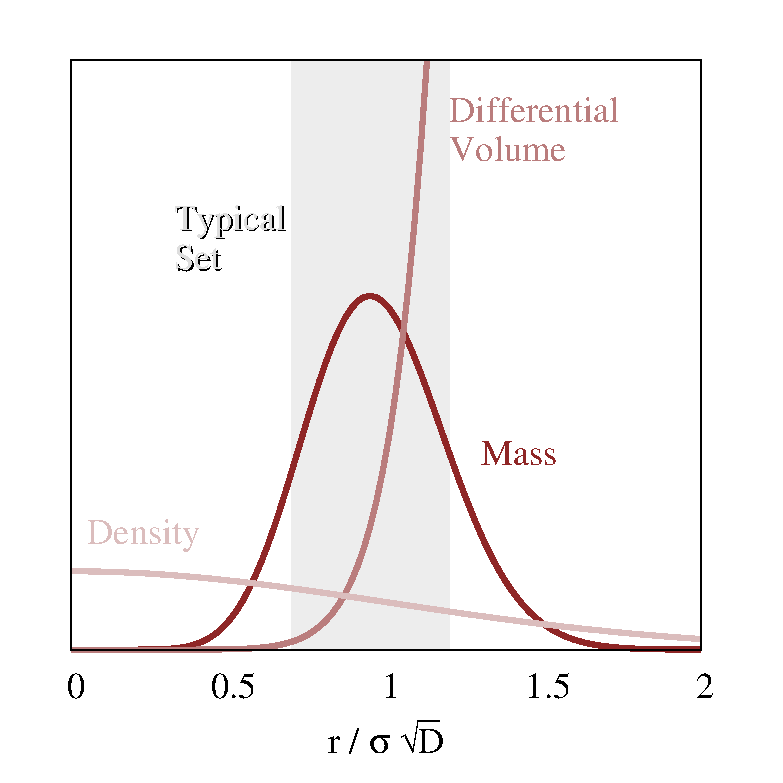
\includegraphics[width=3in]{conc_of_meas_anal.eps}
\caption{In high dimensions real probability distributions generically 
assign almost all of their probability into a singular neighborhood known as
the typical set.  This is apparent even from a probability density function 
representation: although the density concentrates around the corresponding
mode, the volume over which we integrate that density is much larger away
from the mode.  These two opposing trends balance to give the typical set.}
\label{fig:conc_of_meas_anal}
\end{figure*}

Because samples recover all expectations, they too must concentrate 
across the typical set (Figure \ref{fig:samples}).  Consequently, we can also 
use samples to simulate concentration of measure.  For a given $D$ we 
generate a sample from our target probability using a univariate Gaussian 
random number generator available in any computing library,
%
\begin{equation*}
\theta_{d} \sim \mathcal{N} \! \left(0, \sigma^{2} \right),
\end{equation*}
%
and compute the corresponding radial distance 
$r = \sqrt{ \sum_{d = 1}^{D} x_{d}^{2} }$.  Generating a sequence of samples 
and then histogramming the radial distance reveals the same $\chi$ distribution 
that we arrived at analytically (Figure \ref{fig:concentration_of_measure_emp}).

\begin{figure*}
\centering
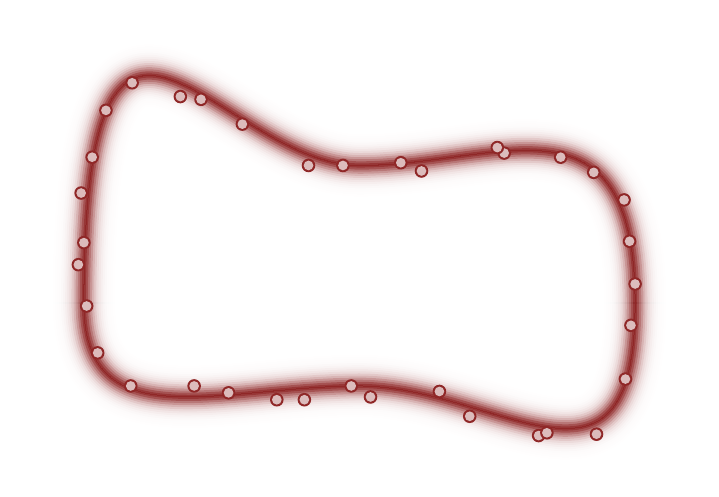
\begin{tikzpicture}[scale=0.35, thick]
  \draw[-,color=white] (-12, 0) to (12, 0);
  
  \begin{scope}
  \clip (-12, -6) rectangle (12, 10);
  \foreach \i in {0, 0.05,..., 1} {
    \draw[line width={30 * \i}, opacity={exp(-8 * \i)}, dark] 
      (-10, 0) .. controls (-10, 15) and (-5, 5) .. (0, 5)
      .. controls (5, 5) and (10, 8) .. (10, 0)
      .. controls (10, -8) and (5, -3) .. (0, -3)
      .. controls (-5, -3) and (-10, -5) .. (-10, 0);
  }
  
  % Mixing
  \fill[color=dark] (-6, -3) circle (7pt);  
  \fill[color=light] (-6, -3) circle (5pt);
  
  \fill[color=dark] (-4.75, -3.25) circle (7pt);  
  \fill[color=light] (-4.75, -3.25) circle (5pt);
  
  \fill[color=dark] (-3, -3.5) circle (7pt);  
  \fill[color=light] (-3, -3.5) circle (5pt);
  
  \fill[color=dark] (-2, -3.5) circle (7pt);  
  \fill[color=light] (-2, -3.5) circle (5pt);
  
  \fill[color=dark] (-0.3, -3) circle (7pt);  
  \fill[color=light] (-0.3, -3) circle (5pt);  
  
  \fill[color=dark] (0.4, -3.4) circle (7pt);  
  \fill[color=light] (0.4, -3.4) circle (5pt);
  
  \fill[color=dark] (2.9, -3.2) circle (7pt);  
  \fill[color=light] (2.9, -3.2) circle (5pt);
  
  \fill[color=dark] (4, -4.1) circle (7pt);  
  \fill[color=light] (4, -4.1) circle (5pt);
  
  \fill[color=dark] (6.5, -4.8) circle (7pt);  
  \fill[color=light] (6.5, -4.8) circle (5pt);
  
  \fill[color=dark] (6.8, -4.7) circle (7pt);  
  \fill[color=light] (6.8, -4.7) circle (5pt);
  
  \fill[color=dark] (8.6, -4.75) circle (7pt);  
  \fill[color=light] (8.6, -4.75) circle (5pt);
  
  \fill[color=dark] (9.65, -2.75) circle (7pt);  
  \fill[color=light] (9.65, -2.75) circle (5pt);
  
  \fill[color=dark] (9.85, -0.8) circle (7pt);  
  \fill[color=light] (9.85, -0.8) circle (5pt);
  
  \fill[color=dark] (10, 0.7) circle (7pt);  
  \fill[color=light] (10, 0.7) circle (5pt);
  
  \fill[color=dark] (9.8, 2.25) circle (7pt);  
  \fill[color=light] (9.8, 2.25) circle (5pt);
  
  \fill[color=dark] (9.6, 3.75) circle (7pt);  
  \fill[color=light] (9.6, 3.75) circle (5pt);
  
  \fill[color=dark] (8.5, 4.75) circle (7pt);  
  \fill[color=light] (8.5, 4.75) circle (5pt);

  \fill[color=dark] (7.3, 5.3) circle (7pt);  
  \fill[color=light] (7.3, 5.3) circle (5pt);
  
  \fill[color=dark] (5.25, 5.45) circle (7pt);  
  \fill[color=light] (5.25, 5.45) circle (5pt);
  
  \fill[color=dark] (5, 5.65) circle (7pt);  
  \fill[color=light] (5, 5.65) circle (5pt);
  
  \fill[color=dark] (2.25, 4.8) circle (7pt);  
  \fill[color=light] (2.25, 4.8) circle (5pt);
  
  \fill[color=dark] (1.5, 5.1) circle (7pt);  
  \fill[color=light] (1.5, 5.1) circle (5pt);
  
  \fill[color=dark] (-0.6, 5) circle (7pt);  
  \fill[color=light] (-0.6, 5) circle (5pt);
  
  \fill[color=dark] (-1.85, 5) circle (7pt);  
  \fill[color=light] (-1.85, 5) circle (5pt);
  
  \fill[color=dark] (-4.25, 6.5) circle (7pt);  
  \fill[color=light] (-4.25, 6.5) circle (5pt);

  \fill[color=dark] (-5.75, 7.4) circle (7pt);  
  \fill[color=light] (-5.75, 7.4) circle (5pt);
  
  \fill[color=dark] (-6.5, 7.5) circle (7pt);  
  \fill[color=light] (-6.5, 7.5) circle (5pt);
  
  \fill[color=dark] (-8.25, 8) circle (7pt);  
  \fill[color=light] (-8.25, 8) circle (5pt);
  
  \fill[color=dark] (-9.2, 7) circle (7pt);  
  \fill[color=light] (-9.2, 7) circle (5pt);
  
  \fill[color=dark] (-9.7, 5.3) circle (7pt);  
  \fill[color=light] (-9.7, 5.3) circle (5pt);
  
  \fill[color=dark] (-10.1, 4) circle (7pt);  
  \fill[color=light] (-10.1, 4) circle (5pt);
  
  \fill[color=dark] (-10, 2.2) circle (7pt);  
  \fill[color=light] (-10, 2.2) circle (5pt);  
  
  \fill[color=dark] (-10.2, 1.4) circle (7pt);  
  \fill[color=light] (-10.2, 1.4) circle (5pt);  

  \fill[color=dark] (-9.9, -0.1) circle (7pt);  
  \fill[color=light] (-9.9, -0.1) circle (5pt);  

  \fill[color=dark] (-9.5, -1.8) circle (7pt);  
  \fill[color=light] (-9.5, -1.8) circle (5pt);  

  \fill[color=dark] (-8.3, -3) circle (7pt);  
  \fill[color=light] (-8.3, -3) circle (5pt);  
  
  \end{scope}
\end{tikzpicture}
\caption{Because samples recover expectations asymptotically,
large sequences of samples must concentrate in the typical set.
This provides a means of visualizing concentration of measure,
and will prove a powerful way to estimate expectations.
}
\label{fig:samples}
\end{figure*}

\begin{figure*}
\centering
\subfigure[]{ 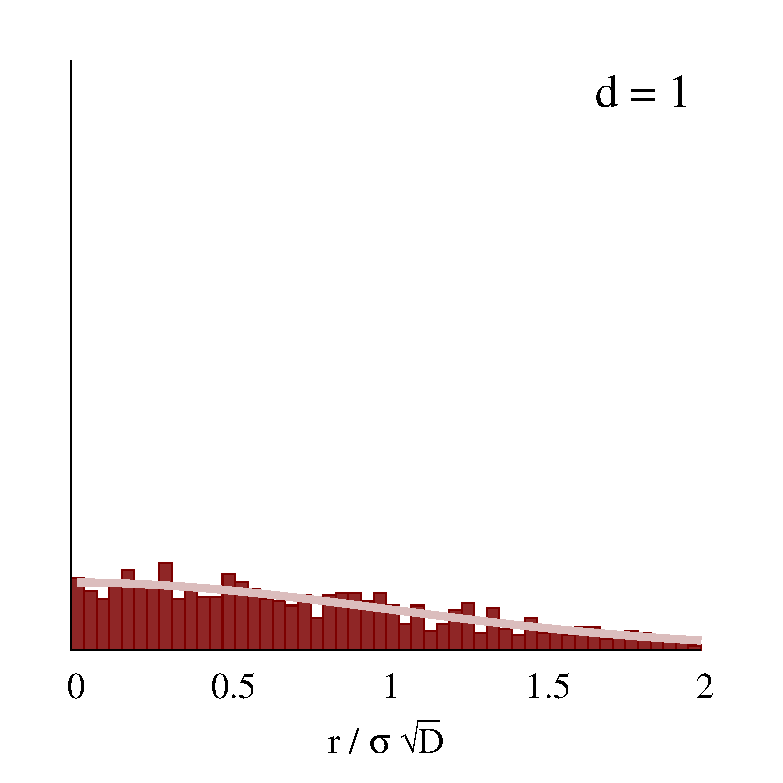
\includegraphics[width=1.85in]{gauss_hist1.eps} }
\subfigure[]{ 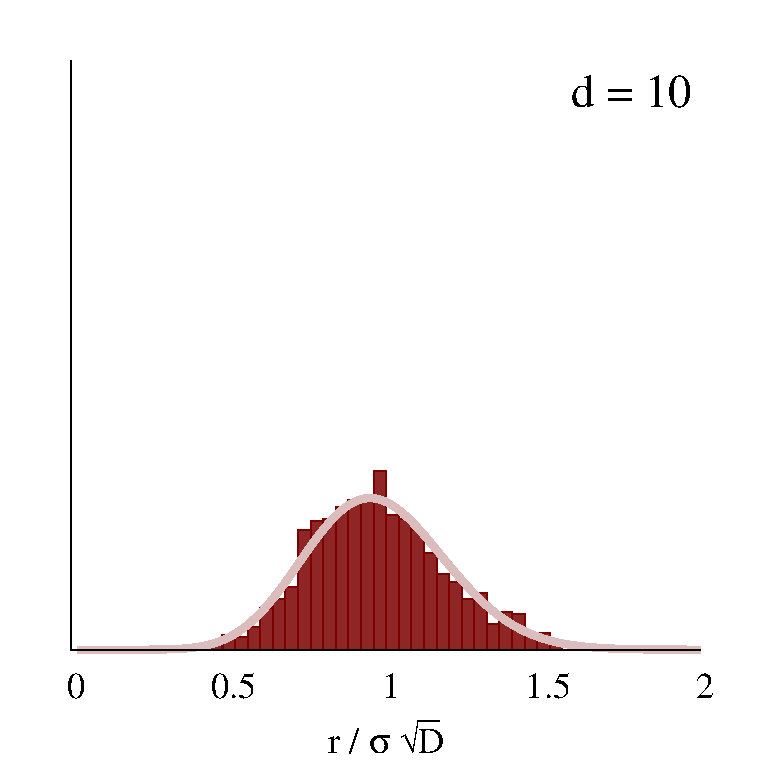
\includegraphics[width=1.85in]{gauss_hist2.eps} }
\subfigure[]{ 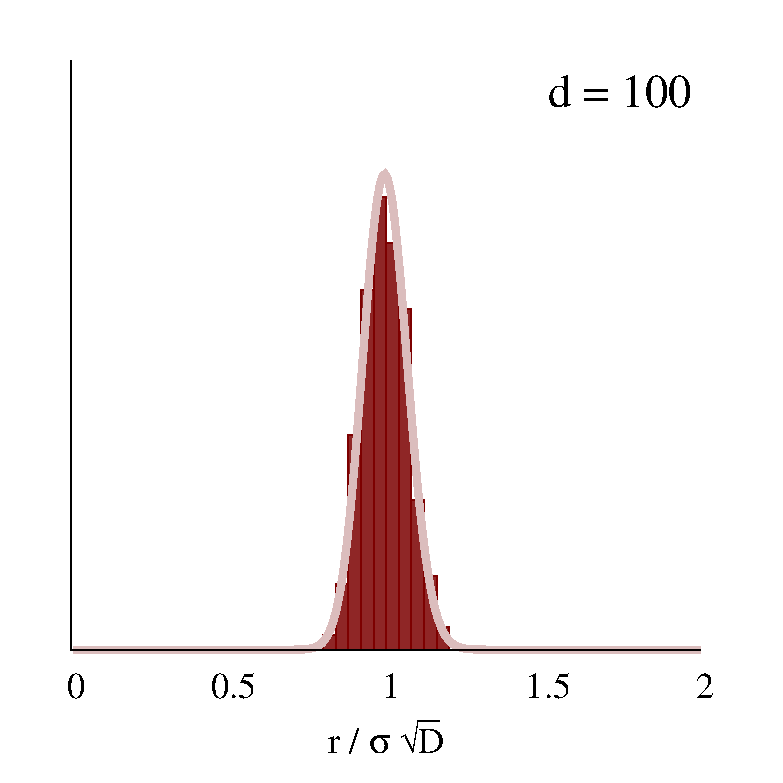
\includegraphics[width=1.85in]{gauss_hist3.eps} }
\caption{Concentration of measure can be visualized with samples 
from a given distribution, which concentrate across the typical set.  
For low-dimensions the concentration is weak and the typical set 
is diffuse, but as the dimensionality of the target distribution grows
so too does the concentration of measure.
}
\label{fig:concentration_of_measure_emp}
\end{figure*}

\chapter{Probability in Practice: Deterministic Estimators}

If we can't compute expectations with respect to our target distribution
analytically, one immediate strategy is to just replace it with a simpler one.  
In other words, we can approximate a complex target distribution, $\PP$, 
with a simpler distribution, $\widetilde{\PP}$, whose expectations, or at 
least some expectations of practical interest, are known analytically,
%
\begin{equation*}
\EE_{\PP} \! \left[ f \right] 
\approx 
\EE_{\widetilde{\PP}} \! \left[ f \right].
\end{equation*}

\emph{Deterministic estimators} use various criteria to identify an 
optimal approximating distribution so that expectations can be 
approximated deterministically.

\section{Modal Estimators}

Ideally all expectations with respect to our approximating distribution 
would be analytic so that we could use it to approximate any 
expectation with respect to our target distribution.  The only
probability distribution that fits this criteria is the \emph{Dirac distribution},
$\mathbb{D}_{\tilde{\theta}}$, that assigns all probability to a single point 
in the sample space, $\tilde{\theta}$,
%
\begin{equation*}
\mathbb{D}_{\tilde{\theta}} \! \left[ E \right] = 
\left\{
\begin{array}{rr}
0, & \tilde{\theta} \notin E  \\
1, & \tilde{\theta} \in E
\end{array}
\right. .
\end{equation*}
%
Because all probability concentrates at $\tilde{\theta}$, expectations 
are trivial,
%
\begin{equation*}
\EE_{\mathbb{D}} \! \left[ f \right] 
=
 f \! \left( \tilde{\theta} \right).
\end{equation*} 

Where, however, should we assign all probability to best approximate
the target distribution and its typical set?  One of the simplest, and 
consequently most popular, deterministic estimation strategies is 
\emph{modal estimation}, where we approximate the target distribution 
with a Dirac distribution at the mode of the probability density function,
%
\begin{equation*}
\hat{\theta} = \mathrm{argmax} \, p \! \left( \theta \right).
\end{equation*}
%
This approach, however, immediately contradicts the intuition provided by 
concentration of measure: it utilizes a single point in the sample space
that lies outside of the typical set and depends entirely on the choice of
probability density function representation!  Why, then, is modal estimation
so ubiquitous?

Modal estimators are seductive because the optimization on which they
rely is relatively computationally inexpensive.  Moreover, in some very 
simple cases modal estimators constructed from the probability density function
in \emph{some} sample spaces can be reasonably accurate for 
\emph{some} functions.  For example, if the target probability distribution 
is sufficiently simple that the typical set is convex \emph{and} if a 
sample space can be found such that the mode of the probability density 
function lies in the center of that typical set, then the corresponding modal 
estimator might yield reasonably accurate estimates for the mean, 
$\EE_{\PP_{\Theta}} \! \left[ \theta \right]$ (Figure \ref{fig:good_map_bad_map}).

\begin{figure*}
\centering
\subfigure[]{
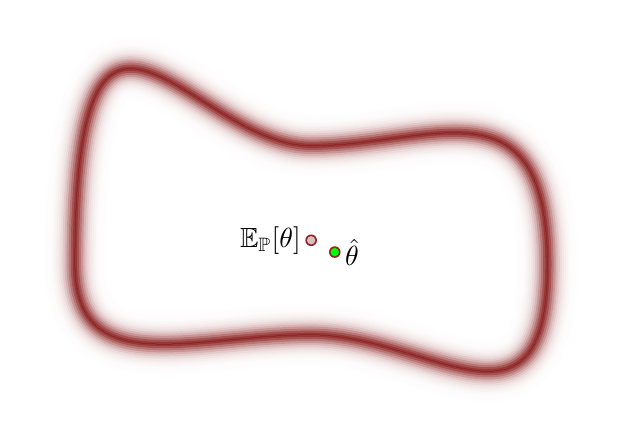
\begin{tikzpicture}[scale=0.3, thick]

  \begin{scope}
    \clip (-12, -6) rectangle (12, 10);
    \foreach \i in {0, 0.05,..., 1} {
      \draw[line width={30 * \i}, opacity={exp(-8 * \i)}, dark] 
        (-10, 0) .. controls (-10, 15) and (-5, 5) .. (0, 5)
        .. controls (5, 5) and (10, 8) .. (10, 0)
        .. controls (10, -8) and (5, -3) .. (0, -3)
        .. controls (-5, -3) and (-10, -5) .. (-10, 0);
    }  
  \end{scope}
  
  \fill[color=dark] (0, 1) circle (7pt);  
  \fill[color=light] (0, 1) circle (5pt)
  node[left, color=black]  { $\EE_{\PP} \! \left[ \theta \right]$ };
 
  \fill[color=dark] (1, 0.5) circle (7pt);
  \fill[color=green] (1, 0.5) circle (5pt)
  node[right, color=black]  { $\hat{\theta}$ };
  
\end{tikzpicture}
}
\subfigure[]{
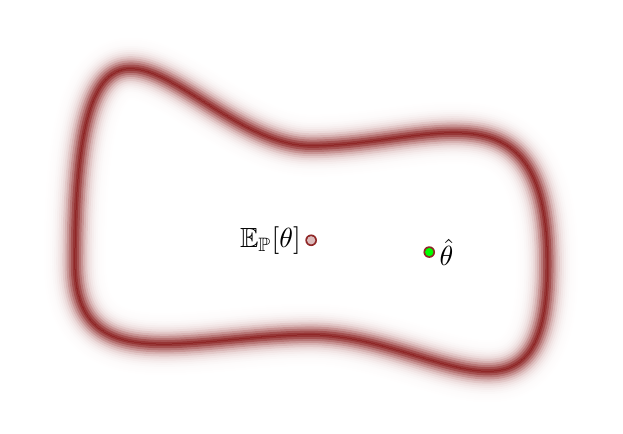
\begin{tikzpicture}[scale=0.3, thick]

  \begin{scope}
    \clip (-12, -6) rectangle (12, 10);
    \foreach \i in {0, 0.05,..., 1} {
      \draw[line width={30 * \i}, opacity={exp(-8 * \i)}, dark] 
        (-10, 0) .. controls (-10, 15) and (-5, 5) .. (0, 5)
        .. controls (5, 5) and (10, 8) .. (10, 0)
        .. controls (10, -8) and (5, -3) .. (0, -3)
        .. controls (-5, -3) and (-10, -5) .. (-10, 0);
    }  
  \end{scope}
  
  \fill[color=dark] (0, 1) circle (7pt);  
  \fill[color=light] (0, 1) circle (5pt)
  node[left, color=black]  { $\EE_{\PP} \! \left[ \theta \right]$ };
 
  \fill[color=dark] (5, 0.5) circle (7pt);
  \fill[color=green] (5, 0.5) circle (5pt)
  node[right, color=black]  { $\hat{\theta}$ };
  
\end{tikzpicture}
}
\caption{(a) In simple cases a prescient choice of sample space can 
yield a modal estimator that well approximates some expectations, 
such as the mean of the real parameters $\theta$.  (b) Poor choices 
of the representation, however, yield very inaccurate estimates, even 
in these simple problems.
}
\label{fig:good_map_bad_map}
\end{figure*}

Because they rely on a point estimate, however, modal estimators are 
terrible at approximating expectations that depend on the breadth of 
the typical set, such as the variance.  Furthermore, identifying the optimal 
sample space for a particular target function, even if one exists, is 
extremely challenging in practice.  Worse, we have no generic means
of even quantifying the error in these estimators for a generic target
distribution.  Ultimately this strong sensitivity to the choice of a particular
expression and the inability to validate the accuracy of the estimators 
makes modal estimation extremely fragile in practice.

\section{Laplace Estimators}

The fragility of modal estimators can be partially resolved by generalizing
them to \emph{Laplace estimators} which approximate the probability
density function with a Gaussian density function,
%
\begin{equation*}
p \! \left( \theta \right) \approx 
\mathcal{N} \! \left( \theta \mid \mu, \Sigma \right),
\end{equation*}
%
where the mean is given by the modal estimate,
%
\begin{equation*}
\mu = \hat{\theta},
\end{equation*}
%
and the covariance is given by the Hessian of the probability density 
function,
%
\begin{equation*}
\left( \Sigma^{-1} \right)_{ij} = 
\frac{ \partial^{2} }{ \partial \theta_{i} \partial \theta_{j} }
p \! \left( \theta \right).
\end{equation*}
%
Expectations are then estimated with Gaussian integrals
%
\begin{equation*}
\mathbb{E}_{\PP} \! \left[ f \right]
\approx 
\int_{\Theta} f \! \left( \theta \right) 
\mathcal{N} \! \left( \theta \mid \mu, \Sigma \right) \dd \theta,
\end{equation*}
%
which often admit analytic solutions.

The accuracy of Laplace approximations depends on how well the
mode and and the Hessian of the probability density function
quantify the geometry of the typical set (Figure \ref{fig:laplace}).
Unfortunately the conditions that are necessary for these estimates
to be reasonably accurate hold only for very simple probability
distributions, and then only if an appropriate sample space can be 
found.  

\begin{figure*}
\centering
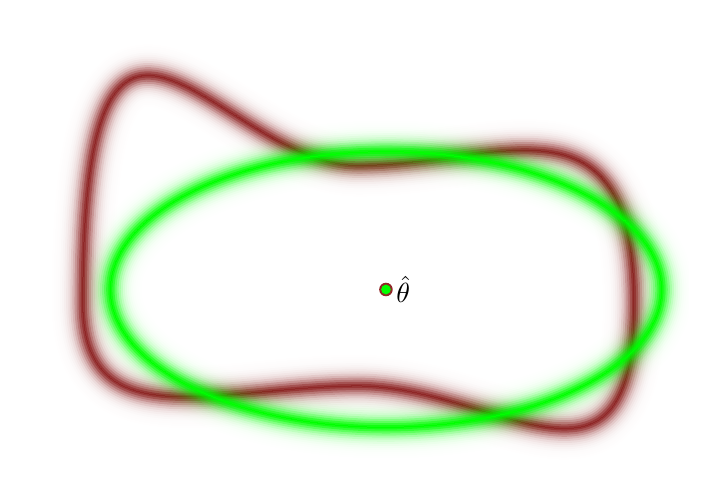
\begin{tikzpicture}[scale=0.35, thick]

  \begin{scope}
    \clip (-12, -6) rectangle (12, 10);
    \foreach \i in {0, 0.05,..., 1} {
      \draw[line width={30 * \i}, opacity={exp(-8 * \i)}, dark] 
        (-10, 0) .. controls (-10, 15) and (-5, 5) .. (0, 5)
        .. controls (5, 5) and (10, 8) .. (10, 0)
        .. controls (10, -8) and (5, -3) .. (0, -3)
        .. controls (-5, -3) and (-10, -5) .. (-10, 0);
    }  
    
    \foreach \i in {0, 0.05,..., 1} {
      \draw[line width={30 * \i}, opacity={exp(-8 * \i)}, green] 
        (1, 0.5) ellipse (10 and 5);
    }
  \end{scope}
 
  \fill[color=dark] (1, 0.5) circle (7pt);
  \fill[color=green] (1, 0.5) circle (5pt)
  node[right, color=black]  { $\hat{\theta}$ };
  
\end{tikzpicture}
\caption{For simple probability distributions with well-chosen
samples spaces, the local geometry around the mode of a 
probability density function can quantify the geometry of the 
entire typical set, yielding accurate Laplace estimators. For
more complex probability distributions, however, this local
information poorly quantifies the global geometry of the 
typical set and Laplace estimators suffer from large biases.
}
\label{fig:laplace}
\end{figure*}

As with the simpler modal estimators, the dependence on the particular
sample space manifests as fragility of the corresponding estimators
and we have no generic means of quantifying the error in practice.  
If we want robust estimation of probabilities and expectations then we 
need strategies that do not depend on these irrelevant properties.

\section{Variational Estimators}

In order to construct an approximation that is not sensitive to the choice 
of a particular sample space we need to frame the problem as an 
optimization over a space of approximating distributions directly.
Optimizations over spaces of probability distributions fall into a class 
of algorithms known as \emph{variational methods}.

Variational methods are characterized by two choices: the variational
family and a divergence function. The \emph{variational family}, 
$\mathcal{Q}$, is a set of probability distributions over the target sample 
space, $\Theta$, such that at least some expectations can be computed
analytically.  In order to identify the best approximation to the target 
distribution we then define a \emph{divergence function},
%
\begin{align*}
D &: 
\mathcal{Q} \times \mathcal{Q}
\rightarrow \mathbb{R}^{+}
\\
& \quad \PP_{1}, \PP_{2} 
\mapsto D \! \left( \PP_{1} \mid\mid \PP_{2} \right),
\end{align*}
%
which is zero if the two arguments are the same and increases as they 
deviate from each other more strongly.

The best approximating distribution is then defined by the variational 
objective (Figure \ref{fig:variational_cartoon}).
%
\begin{equation*}
\mathbb{Q}^{*}
= 
\underset{\mathbb{Q} \in \mathcal{Q}}{\mathrm{argmin}} \,
D \! \left( \PP \mid\mid \mathbb{Q} \right).
\end{equation*}
%
Although straightforward to define, this variational optimization can be
quite challenging in practice.  Depending on how the target distribution
interacts with the choice of variational distribution and divergence
function, the variational objective might feature multiple critical points
and we may not be able to find the global optimum in practice
(Figure \ref{fig:variational_challenges}).

\begin{figure*}
\centering
%
\subfigure[]{
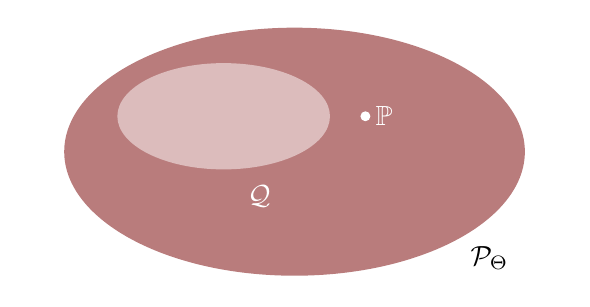
\begin{tikzpicture}[scale=0.225, thick]
  
  \draw[color=white] (-15, 0) -- (15, 0);
  
  \fill[mid] (0, 0) ellipse (13 and 7);
  \node at (11, -6) {$\mathcal{P}_{\Theta}$};
  
  \fill[light] (-4, 2) ellipse (6 and 3);
  \node[color=white] at (-2, -2.5) {$\mathcal{Q}$};
  
  \fill[color=white] (4, 2) circle (8pt)
  node[right, color=white] {$\PP$};
  
\end{tikzpicture}
}
\subfigure[]{
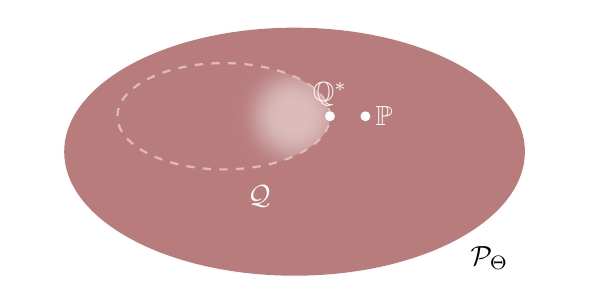
\begin{tikzpicture}[scale=0.225, thick]

  \draw[color=white] (-15, 0) -- (15, 0);
  
  \fill[mid] (0, 0) ellipse (13 and 7);
  \node at (11, -6) {$\mathcal{P}_{\Theta}$};
  
  \draw[color=light, dashed] (-4, 2) ellipse (6 and 3);
  \node[color=white] at (-2, -2.5) {$\mathcal{Q}$};
  
  \begin{scope}
    \clip (-4, 2) ellipse (6 and 3);
    \foreach \i in {0, 0.05,..., 1} {
      \fill[opacity={exp(-5 * \i*\i)}, light] (0, 2) circle ({4 * \i});      
    }
  \end{scope}
  
  \fill[color=white] (2, 2) circle (8pt)
  node[above, color=white] {$\mathbb{Q}^{*}$};
  
  \fill[color=white] (4, 2) circle (8pt)
  node[right, color=white] {$\PP$};
  
\end{tikzpicture}
}
\caption{(a) A variational family, $\mathcal{Q}$, is a set of probability distributions
taken from the set of all probability distributions over the same sample space, as 
the target distribution, $\mathcal{P}_{\Theta}$.  (b) Adding a divergence function 
distinguishes which elements of $\mathcal{Q}$ are good approximations to the 
target distribution, allowing us to identify the best approximation, $\mathbb{Q}^{*}$.
}
\label{fig:variational_cartoon}
\end{figure*}

\begin{figure*}
\centering
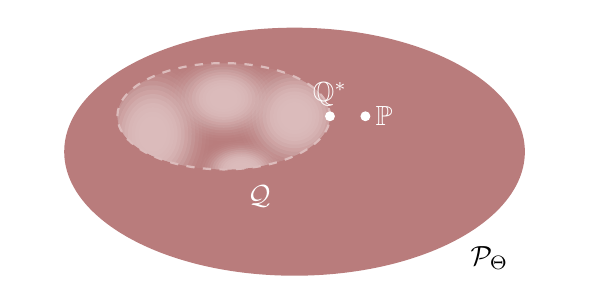
\begin{tikzpicture}[scale=0.225, thick]

  \draw[color=white] (-15, 0) -- (15, 0);
  
  \fill[mid] (0, 0) ellipse (13 and 7);
  \node at (11, -6) {$\mathcal{P}_{\Theta}$};
  
  \draw[color=light, dashed] (-4, 2) ellipse (6 and 3);
  \node[color=white] at (-2, -2.5) {$\mathcal{Q}$};
  
  \begin{scope}
    \clip (-4, 2) ellipse (6 and 3);
    
    \foreach \i in {0, 0.05,..., 1} {
      \fill[opacity={exp(-5 * \i*\i)}, light] (0, 2) circle ({4 * \i});      
    }
    
    \foreach \i in {0, 0.05,..., 1} {
      \fill[opacity={exp(-5 * \i*\i)}, light] (-4, 3) ellipse ({4 * \i} and {3 * \i});      
    }
    
    \foreach \i in {0, 0.05,..., 1} {
      \fill[opacity={exp(-5 * \i*\i)}, light] (-8, 1) ellipse ({4 * \i} and {5 * \i});      
    }
    
    \foreach \i in {0, 0.05,..., 1} {
      \fill[opacity={exp(-5 * \i*\i)}, light] (-3, -1) ellipse ({3 * \i} and {2 * \i});      
    }
  \end{scope}
  
  \fill[color=white] (2, 2) circle (8pt)
  node[above, color=white] {$\mathbb{Q}^{*}$};
  
  \fill[color=white] (4, 2) circle (8pt)
  node[right, color=white] {$\PP$};
  
\end{tikzpicture}
\caption{Typically different elements of the variational family are able to 
capture different characteristics of the target distribution and the variational 
objective manifests multiple optima.  Even if a global optimum, $\mathbb{Q}^{*}$, 
exists it will be difficult to find and we may be left with only a suboptimal local 
optimum.
}
\label{fig:variational_challenges}
\end{figure*}

Even if we could find the best approximating distribution, however,
there are no guarantees that it will yield accurate estimates for
all relevant expectations of our target distribution.  For example, 
some divergence functions are biased towards variational solutions
that underestimate the breadth of the typical set while others
tend to significantly overestimate it (Figure \ref{fig:variational_approximations}).

Variational methods are relatively new to statistics and at the moment
there are no generic methods for quantifying the error in variational
estimators.

\begin{figure*}
\centering
\subfigure[]{
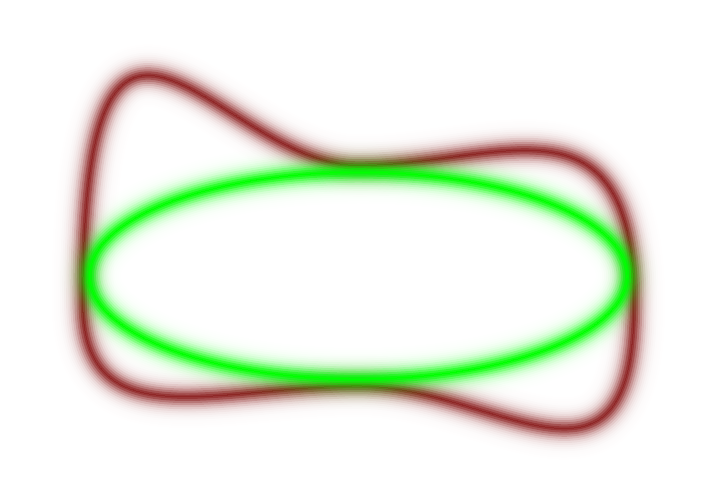
\begin{tikzpicture}[scale=0.35, thick]
  \begin{scope}
    \clip (-12, -6) rectangle (12, 10);
    \foreach \i in {0, 0.05,..., 1} {
      \draw[line width={30 * \i}, opacity={exp(-8 * \i)}, dark] 
        (-10, 0) .. controls (-10, 15) and (-5, 5) .. (0, 5)
        .. controls (5, 5) and (10, 8) .. (10, 0)
        .. controls (10, -8) and (5, -3) .. (0, -3)
        .. controls (-5, -3) and (-10, -5) .. (-10, 0);
    }  
    
    \foreach \i in {0, 0.05,..., 1} {
      \draw[line width={30 * \i}, opacity={exp(-8 * \i)}, green] 
        (0, 1) ellipse (9.75 and 3.75);
    }
  \end{scope}
\end{tikzpicture}
}
\subfigure[]{
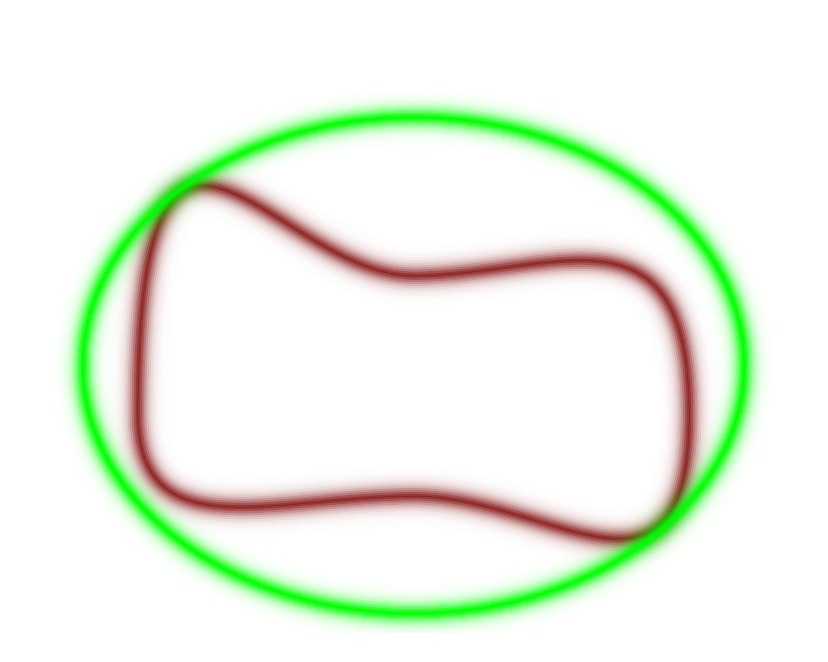
\begin{tikzpicture}[scale=0.35, thick]
  \begin{scope}
    \clip (-14, -8) rectangle (14, 14);
    \foreach \i in {0, 0.05,..., 1} {
      \draw[line width={30 * \i}, opacity={exp(-8 * \i)}, dark] 
        (-10, 0) .. controls (-10, 15) and (-5, 5) .. (0, 5)
        .. controls (5, 5) and (10, 8) .. (10, 0)
        .. controls (10, -8) and (5, -3) .. (0, -3)
        .. controls (-5, -3) and (-10, -5) .. (-10, 0);
    }  
    
    \foreach \i in {0, 0.05,..., 1} {
      \draw[line width={30 * \i}, opacity={exp(-8 * \i)}, green] 
        (0, 1.75) ellipse (12 and 9);
    }
  \end{scope}
\end{tikzpicture}
}
\caption{Intuition about the effects of a particular variational divergence 
function can be developed by considering how the typical set of an
approximating distribution (green) interacts with the typical of the target 
distribution (red).  (a) Some divergence functions favor approximating
distributions that expand into the interior of the target typical set,
resulting in an underestimate of the breadth of the typical set.  (b)
Others, however, favor approximating distractions that collapse around
the exterior of the target typical set, resulting in overestimated expectations.
}
\label{fig:variational_approximations}
\end{figure*}
\chapter{Probability in Practice: Stochastic Estimators}

The accuracy of deterministic estimators will always be limited by
the flexibility of the approximating distribution to match the geometry 
of the typical set of the target distribution.  The only way to overcome
this restriction is to quantify the typical set of the target distribution
directly.  Unfortunately, this presents problems of its own as in practice 
we don't know where to find the typical set in the expansive sample space.  
Because exhaustive search of the sample space is far too expensive
we need a more targeted procedure for finding and then exploring 
the typical set.

By construction an infinite number of samples from the target distribution 
quantifies the typical set, and hence the samples themselves provide
a natural way to identify the typical set (Figure \ref{fig:samples}).  The
utility of samples, however, depends both on how precisely we can 
quantify the typical set using only a finite number of samples and how
well we can generate samples in the first place.

\emph{Stochastic estimators} use samples, either from the target probability
distribution or auxiliary probability distributions, to construct estimators 
of the expectation with respect to the target distribution.  Exactly how these
samples are generated leads to estimators with substantially different 
behaviors.

\subsection{Monte Carlo Estimators}

Monte Carlo estimators use a finite sequence of exact samples from
the target distribution to estimate expectations.  Given a sequence
of exact samples $\left\{ \theta_{1}, \ldots, \theta_{N} \right\}$ we can
construct a  \emph{Monte Carlo estimator} of the expectation of 
\emph{any} function $f : \Theta \rightarrow \RR$ as
%
\begin{equation*}
\hat{f}^{\mathrm{MC}}_{N} \equiv
\frac{1}{N} \sum_{n = 1}^{N} f \! \left( \theta_{n} \right).
\end{equation*}

By construction these Monte Carlo estimators recover the exact
expectation asymptotically,
%
\begin{equation*}
\lim_{N \rightarrow \infty} \hat{f}^{\mathrm{MC}}_{N}
=
\EE_{\PP} [ f ],
\end{equation*}
%
but they are also accurate even when the sequence is finite.
Provided that the samples are exact, Monte Carlo estimators 
follow a Central Limit Theorem -- for sufficiently large $N$ the 
estimators themselves follow a distribution given by a Gaussian 
density,
%
\begin{equation*}
\hat{f}_{N} \sim 
\mathcal{N} \! \left( \EE_{\PP} [ f ],
\mathrm{MCSE} \right),
\end{equation*}
%
where the \emph{Monte Carlo Standard Error} is defined as
%
\begin{equation*}
\mathrm{MCSE } \equiv \sqrt{ \frac{ \mathrm{Var} [ f ] }{N} }.
\end{equation*}
%
Consequently Monte Carlo estimators are unbiased with respect
to all of the possible sequences we could have generated, and 
their precision improves as we generate more and more samples.
Moreover, functions with high variance are more challenging to
estimate than those with low variance.

In practice we use another Monte Carlo estimator to approximate the
variance $\mathrm{Var} [ f ] $, and hence the Monte Carlo Standard
Error itself.  The error of this approximation is
%
\begin{equation*}
\sqrt{\mathrm{Var} [ \, \mathrm{Var} [ f ]  \, ] / N^{2} },
\end{equation*}
which is typically negligible compared to the Monte Carlo Standard Error 
of $f$.  Monte Carlo estimators, then, are distinct from deterministic 
approximations in that they naturally come equipped with a procedure 
for at least estimating their error.

Of course all of these benefits of Monte Carlo estimators are dependent 
on our ability to generate exact samples from the target probability 
distribution.  Unfortunately, generating exact samples is infeasible for all 
but the simplest probability distributions, and we are once again frustrated 
by our ignorance of the typical set.  In order to proceed we need to 
approximate exact samples themselves.

\subsection{Importance Sampling Estimators}

Although we typically can't generate exact samples from the target 
distribution, often we can generate exact samples from an 
\emph{auxiliary} probability distribution, $\mathbb{G}$,
%
\begin{equation*}
\left\{ \vartheta_{1}, \ldots, \vartheta_{N} \right\} \sim \mathbb{G}.
\end{equation*}
%
\emph{Importance sampling estimators} use these auxiliary samples 
corrected with \emph{importance weights}, $w \! \left( \vartheta \right)$,  
%
\begin{equation*}
\EE_{\PP} [ f ] \approx 
\hat{f}^{\mathrm{IS}}_{N} = 
\frac{1}{N} \sum_{n = 1}^{N} 
w \! \left( \vartheta_{n} \right) f \! \left( \vartheta_{n} \right)
\end{equation*}
%
If $p$ and $g$ are the probability density functions corresponding to
the target distribution and auxiliary distribution, respectively, then the 
importance weights are given by
%
\begin{equation*}
w \! \left( \vartheta_{n} \right) =
\frac{ p \! \left( \vartheta_{n} \right) }
{ g \! \left( \theta_{n} \right) }.
\end{equation*}
%
Although they are constructed from probability density functions, 
importance weights, and hence importance sampling estimators,
are invariant to the choice of sample space.  When we map to
an equivalent sample space, the resulting Jacobian is the same
in both the numerator and denominator and consequently cancels 
when evaluating the weights themselves.

Given certain regularity conditions, importance sampling estimators 
also satisfy a Central Limit Theorem
%
\begin{equation*}
\hat{f}_{N}^{\mathrm{IS}} \sim 
\mathcal{N} \! \left( \EE_{\PP} [ f ],
\mathrm{ISSE} \right),
\end{equation*}
%
The \emph{Importance Sampling Standard Error} is given by
%
\begin{equation*}
\mathrm{ISSE} \equiv \sqrt{ \frac{ \mathrm{Var} [ f ] }{\mathrm{ESS} } },
\end{equation*}
%
with the \emph{effective sample size} defined as
%
\begin{equation*}
\mathrm{ESS} = 
N 
\frac{ \left( \sum_{n = 1}^{N} w \! \left( \vartheta_{n} \right) \right)^{2} }
{ \sum_{n = 1}^{N} w \! \left( \vartheta_{n} \right)^{2} }.
\end{equation*}
%
Comparing this to the Monte Carlo Central Limit Theorem we can
see that the effective sample size quantifies how many exact
samples would have yielded the same estimator precision,
hence the effective sample size can be interpreted as the
effective number of exact samples ``contained'' in the auxiliary
samples.

The challenge with constructing a useful importance sampler is
finding an auxiliary distribution that is not too different from the
target distribution.  Although importance sampling estimators are 
unbiased, their variance can be so large as to be impractical when 
the auxiliary distribution deviates too strongly from the target distribution 
and the weights are large.  In fact, when the auxiliary distribution has 
lighter tails than the target distribution these estimators can 
easily have infinitely large variance: not only does this make 
the estimators themselves useless, it also makes estimates of 
the variance and hence any quantification of the estimator error 
useless.

Selecting an auxiliary distribution that yields accurate importance
sampling estimators, however, is challenging without knowing
the structure of the typical set a priori.  Ultimately, importance
sampling is most useful as a means to correct a distribution that 
is already known to be a good approximation to the target
distribution.

\subsection{Markov Chain Monte Carlo Estimators}

Another strategy for approximating the Monte Carlo procedure
is to generate samples from the target distribution but relax
the requirement that they be exact.  Fortunately, correlated 
samples are readily given by \emph{Markov chains}.

A Markov chain is a stochastic processes generated not by a
static probability distribution but by a probability distribution 
that depends on the last state in the sequence.  In other words, 
each state in the sequence is sampled from a conditional 
probability distribution known as a \emph{Markov transition 
kernel}, $\mathbb{T}$, 
%
\begin{align*}
\mathbb{T}
&: \EV{\Theta} \times \Theta \rightarrow \left[0, 1 \right] \\
&\quad \left( E, \theta \right) \;\; \mapsto 
\mathbb{T} \! \left[ E \mid \theta \right].
\end{align*}
%
When the Markov transition operator preserves the target
distribution,
%
\begin{equation*}
\PP \! \left[ E \right]
=
\mathbb{E}_{\PP} \! 
\left[  \mathbb{T} \! \left[ E \mid \theta \right] \right]
\end{equation*}
%
or, with respect to probability density functions,
%
\begin{equation*}
p \! \left( \theta \right)
=
\int_{\Theta} t \! \left( \theta' \mid \theta \right) 
\pi \! \left( \theta' \right) \dd \theta',
\end{equation*}
%
then the Markov chain asymptotically recovers expectations
with \emph{Markov chain Monte Carlo estimators},
%
\begin{equation*}
\lim_{N \rightarrow \infty} 
\hat{f}^{\mathrm{MCMC}}_{N}
\equiv
\lim_{N \rightarrow \infty} 
\frac{1}{N} \sum_{n = 1}^{N} f \! \left( \theta_{n} \right)
=
\mathbb{E}_{\PP} \! \left[ f \right],
\end{equation*}
%
and we can interpret the Markov chain itself as a sequence
of correlated samples from the target distribution.

More intuitively, the Markov transition kernel quantifies
the variability in each step of the Markov chain.  When the
transition preserves the target distribution, then it 
concentrates closer to the typical set than away from it --
it is literally attracted to the typical set.  Consequently, the
Markov chain will eventually find and then explore the
typical set no matter where we start in the sample space,
and the Markov chain Monte Carlo estimators will converge
to the true expectations.
 
The important caveat here is that the Markov chain is 
guaranteed to find and fully explore the typical set only 
asymptotically.  In practice, however, it is the only the finite time 
performance of Markov chains that matters and, unfortunately, the 
finite time behavior of Markov chain Monte Carlo is much more
subtle than its exact predecessor.

In this section we discuss how Markov chain Monte Carlo
behaves under ideal conditions, how it behaves under
less-than-ideal conditions, and how to effectively run
the algorithm in practice to be robust to the latter.

\subsubsection{Markov Chain Monte Carlo Under Ideal Conditions}

Under ideal conditions, Markov chains explore the target
distribution in three distinct phases.  In the first phase the
Markov chain converges towards the typical set from its
initial position and Markov chain Monte Carlo estimators
are highly biased (Figure \ref{fig:ideal_mcmc}a).  The
second phase begins once the Markov chain finds the
typical set and persists through the first sojourn across
the typical set.  This initial exploration is extremely effective
and the accuracy of Markov chain Monte Carlo estimators
rapidly improves as the bias from the initial samples is
eliminated (Figure \ref{fig:ideal_mcmc}b).  The third phase 
consists of all subsequent exploration where the the Markov 
chain refines its exploration of the typical set and the precision 
of the Markov chain Monte Carlo estimators improves, albeit 
at a slower rate (Figure \ref{fig:ideal_mcmc}c).

\begin{figure*}
\centering
\subfigure[]{
\begin{tikzpicture}[scale=0.25, thick]
  \draw[-,color=white] (-12, 0) to (12, 0);
  
  \begin{scope}
  \clip (-12, -10) rectangle (12, 10);
  
  \foreach \i in {0, 0.05,..., 1} {
    \draw[line width={30 * \i}, opacity={exp(-8 * \i)}, dark] 
      (-10, 0) .. controls (-10, 15) and (-5, 5) .. (0, 5)
      .. controls (5, 5) and (10, 8) .. (10, 0)
      .. controls (10, -8) and (5, -3) .. (0, -3)
      .. controls (-5, -3) and (-10, -5) .. (-10, 0);
  }

  %\fill[color=dark] (-11, -8) circle (7pt);  
  %\fill[color=light] (-11, -8) circle (5pt);
  
  \fill[color=dark] (-10, -6.5) circle (7pt);  
  \fill[color=light] (-10, -6.5) circle (5pt);
  
  \fill[color=dark] (-9, -6.75) circle (7pt);  
  \fill[color=light] (-9, -6.75) circle (5pt);
  
  \fill[color=dark] (-8.25, -5) circle (7pt);  
  \fill[color=light] (-8.25, -5) circle (5pt);
  
  \fill[color=dark] (-7.5, -4) circle (7pt);  
  \fill[color=light] (-7.5, -4) circle (5pt);
  
  \fill[color=dark] (-7, -3.5) circle (7pt);  
  \fill[color=light] (-7, -3.5) circle (5pt);
  
  \fill[color=dark] (-6.5, -3.6) circle (7pt);  
  \fill[color=light] (-6.5, -3.6) circle (5pt);  
  
  \end{scope}
  
  \draw[-,color=white] (14, 0) to (38, 0);  
  \node[] at (28,3) {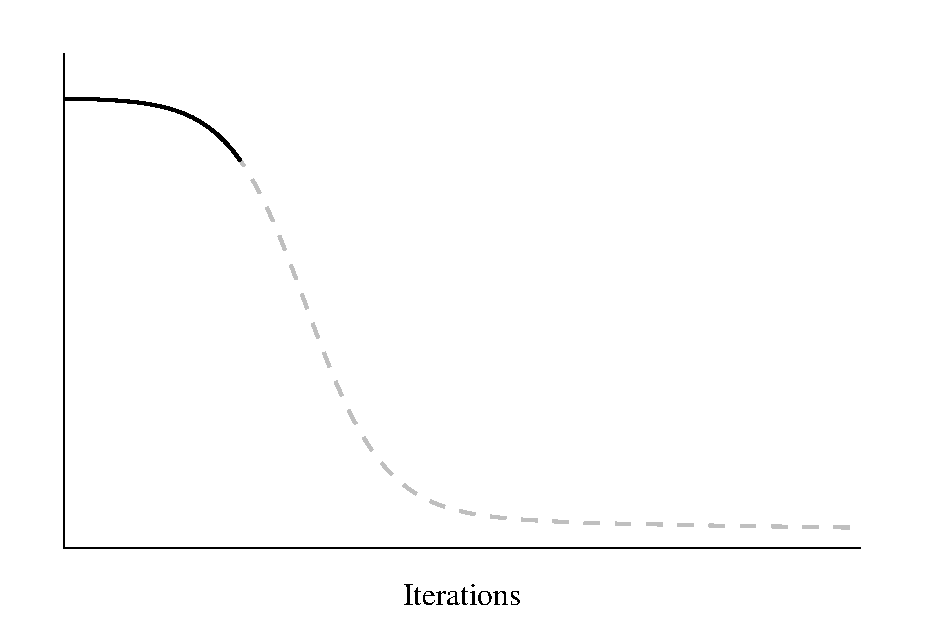
\includegraphics[width=5cm]{convergence1.eps}};
  \node[rotate=90] at (15.5,3) { $\left| \mathbb{E} \! \left[ f \right] - \hat{f} \right|$ };
\end{tikzpicture}
}
\subfigure[]{
\begin{tikzpicture}[scale=0.25, thick]
  \draw[-,color=white] (-12, 0) to (12, 0);
  
  \begin{scope}
  \clip (-12, -10) rectangle (12, 10);
  \foreach \i in {0, 0.05,..., 1} {
    \draw[line width={30 * \i}, opacity={exp(-8 * \i)}, dark] 
      (-10, 0) .. controls (-10, 15) and (-5, 5) .. (0, 5)
      .. controls (5, 5) and (10, 8) .. (10, 0)
      .. controls (10, -8) and (5, -3) .. (0, -3)
      .. controls (-5, -3) and (-10, -5) .. (-10, 0);
  }
  
  % Convergence
  
  %\fill[color=dark] (-11, -8) circle (7pt);  
  %\fill[color=light] (-11, -8) circle (5pt);
  
  \fill[color=dark] (-10, -6.5) circle (7pt);  
  \fill[color=light] (-10, -6.5) circle (5pt);
  
  \fill[color=dark] (-9, -6.75) circle (7pt);  
  \fill[color=light] (-9, -6.75) circle (5pt);
  
  \fill[color=dark] (-8.25, -5) circle (7pt);  
  \fill[color=light] (-8.25, -5) circle (5pt);
  
  \fill[color=dark] (-7.5, -4) circle (7pt);  
  \fill[color=light] (-7.5, -4) circle (5pt);
  
  \fill[color=dark] (-7, -3.5) circle (7pt);  
  \fill[color=light] (-7, -3.5) circle (5pt);
  
  \fill[color=dark] (-6.5, -3.6) circle (7pt);  
  \fill[color=light] (-6.5, -3.6) circle (5pt);  
  
  % Mixing
  
  \fill[color=dark] (-6, -3) circle (7pt);  
  \fill[color=light] (-6, -3) circle (5pt);
  
  %\fill[color=dark] (-5.5, -3.5) circle (7pt);  
  %\fill[color=light] (-5.5, -3.5) circle (5pt);
  
  %\fill[color=dark] (-5, -3.75) circle (7pt);  
  %\fill[color=light] (-5, -3.75) circle (5pt);
  
  \fill[color=dark] (-4.75, -3.25) circle (7pt);  
  \fill[color=light] (-4.75, -3.25) circle (5pt);
  
  %\fill[color=dark] (-5, -3.5) circle (7pt);  
  %\fill[color=light] (-5, -3.5) circle (5pt);  
  
  %\fill[color=dark] (-4, -3.8) circle (7pt);  
  %\fill[color=light] (-4, -3.8) circle (5pt);
  
  \fill[color=dark] (-3, -3.5) circle (7pt);  
  \fill[color=light] (-3, -3.5) circle (5pt);
  
  %\fill[color=dark] (-2.8, -3) circle (7pt);  
  %\fill[color=light] (-2.8, -3) circle (5pt);
  
  %\fill[color=dark] (-2.9, -3.3) circle (7pt);  
  %\fill[color=light] (-2.9, -3.3) circle (5pt);  
  
  \fill[color=dark] (-2, -3.5) circle (7pt);  
  \fill[color=light] (-2, -3.5) circle (5pt);
  
  %\fill[color=dark] (-1.25, -3) circle (7pt);  
  %\fill[color=light] (-1.25, -3) circle (5pt);
  
  %\fill[color=dark] (-0.5, -2.75) circle (7pt);  
  %\fill[color=light] (-0.5, -2.75) circle (5pt);
  
  \fill[color=dark] (-0.3, -3) circle (7pt);  
  \fill[color=light] (-0.3, -3) circle (5pt);  
  
  %\fill[color=dark] (0.1, -2.75) circle (7pt);  
  %\fill[color=light] (0.1, -2.75) circle (5pt);
  
  %\fill[color=dark] (0.15, -3.1) circle (7pt);  
  %\fill[color=light] (0.15, -3.1) circle (5pt);  
  
  \fill[color=dark] (0.4, -3.4) circle (7pt);  
  \fill[color=light] (0.4, -3.4) circle (5pt);
  
  %\fill[color=dark] (1.1, -3.25) circle (7pt);  
  %\fill[color=light] (1.1, -3.25) circle (5pt);
  
  %\fill[color=dark] (2.7, -3.45) circle (7pt);  
  %\fill[color=light] (2.7, -3.45) circle (5pt);
  
  \fill[color=dark] (2.9, -3.2) circle (7pt);  
  \fill[color=light] (2.9, -3.2) circle (5pt);
  
  %\fill[color=dark] (3.1, -3.7) circle (7pt);  
  %\fill[color=light] (3.1, -3.7) circle (5pt);
  
  %\fill[color=dark] (4.2, -3.9) circle (7pt);  
  %\fill[color=light] (4.2, -3.9) circle (5pt);
  
  \fill[color=dark] (4, -4.1) circle (7pt);  
  \fill[color=light] (4, -4.1) circle (5pt);
  
  %\fill[color=dark] (5, -4) circle (7pt);  
  %\fill[color=light] (5, -4) circle (5pt);
  
  %\fill[color=dark] (5.8, -4.3) circle (7pt);  
  %\fill[color=light] (5.8, -4.3) circle (5pt);
  
  \fill[color=dark] (6.5, -4.8) circle (7pt);  
  \fill[color=light] (6.5, -4.8) circle (5pt);
  
  %\fill[color=dark] (6.8, -4.5) circle (7pt);  
  %\fill[color=light] (6.8, -4.5) circle (5pt);
  
  %\fill[color=dark] (7, -4.6) circle (7pt);  
  %\fill[color=light] (7, -4.6) circle (5pt);
  
  \fill[color=dark] (6.8, -4.7) circle (7pt);  
  \fill[color=light] (6.8, -4.7) circle (5pt);
  
  %\fill[color=dark] (7.75, -4.2) circle (7pt);  
  %\fill[color=light] (7.75, -4.2) circle (5pt);
  
  %\fill[color=dark] (8.5, -4.25) circle (7pt);  
  %\fill[color=light] (8.5, -4.25) circle (5pt);
  
  \fill[color=dark] (8.6, -4.75) circle (7pt);  
  \fill[color=light] (8.6, -4.75) circle (5pt);
  
  %\fill[color=dark] (8.8, -4.5) circle (7pt);  
  %\fill[color=light] (8.8, -4.5) circle (5pt);
  
  %\fill[color=dark] (9.25, -3.5) circle (7pt);  
  %\fill[color=light] (9.25, -3.5) circle (5pt);
  
  \fill[color=dark] (9.65, -2.75) circle (7pt);  
  \fill[color=light] (9.65, -2.75) circle (5pt);
  
  %\fill[color=dark] (9.5, -2) circle (7pt);  
  %\fill[color=light] (9.5, -2) circle (5pt);

  %\fill[color=dark] (9.8, -3) circle (7pt);  
  %\fill[color=light] (9.8, -3) circle (5pt);
  
  \fill[color=dark] (9.85, -0.8) circle (7pt);  
  \fill[color=light] (9.85, -0.8) circle (5pt);
  
  %\fill[color=dark] (10.1, -0.4) circle (7pt);  
  %\fill[color=light] (10.1, -0.4) circle (5pt);

  %\fill[color=dark] (10.25, 0.3) circle (7pt);  
  %\fill[color=light] (10.25, 0.3) circle (5pt);
  
  \fill[color=dark] (10, 0.7) circle (7pt);  
  \fill[color=light] (10, 0.7) circle (5pt);
  
  %\fill[color=dark] (9.7, 0.9) circle (7pt);  
  %\fill[color=light] (9.7, 0.9) circle (5pt);
  
  %\fill[color=dark] (10.3, 1.4) circle (7pt);  
  %\fill[color=light] (10.3, 1.4) circle (5pt);
  
  \fill[color=dark] (9.8, 2.25) circle (7pt);  
  \fill[color=light] (9.8, 2.25) circle (5pt);
  
  %\fill[color=dark] (10, 2.5) circle (7pt);  
  %\fill[color=light] (10, 2.5) circle (5pt);
  
  %\fill[color=dark] (10, 3) circle (7pt);  
  %\fill[color=light] (10, 3) circle (5pt);
  
  \fill[color=dark] (9.6, 3.75) circle (7pt);  
  \fill[color=light] (9.6, 3.75) circle (5pt);
  
  %\fill[color=dark] (9.1, 4.4) circle (7pt);  
  %\fill[color=light] (9.1, 4.4) circle (5pt);
  
  %\fill[color=dark] (9.1, 4.1) circle (7pt);  
  %\fill[color=light] (9.1, 4.1) circle (5pt);
  
  \fill[color=dark] (8.5, 4.75) circle (7pt);  
  \fill[color=light] (8.5, 4.75) circle (5pt);
  
  %\fill[color=dark] (8.1, 5.75) circle (7pt);  
  %\fill[color=light] (8.1, 5.75) circle (5pt);
  
  %\fill[color=dark] (7.7, 5.2) circle (7pt);  
  %\fill[color=light] (7.7, 5.2) circle (5pt);
  
  \fill[color=dark] (7.3, 5.3) circle (7pt);  
  \fill[color=light] (7.3, 5.3) circle (5pt);
  
  %\fill[color=dark] (6.6, 5.8) circle (7pt);  
  %\fill[color=light] (6.6, 5.8) circle (5pt);
  
  %\fill[color=dark] (6, 6) circle (7pt);  
  %\fill[color=light] (6, 6) circle (5pt);
  
  \fill[color=dark] (5.25, 5.45) circle (7pt);  
  \fill[color=light] (5.25, 5.45) circle (5pt);
  
  %\fill[color=dark] (4.75, 5.75) circle (7pt);  
  %\fill[color=light] (4.75, 5.75) circle (5pt);
  
  %\fill[color=dark] (3.5, 5.28) circle (7pt);  
  %\fill[color=light] (3.5, 5.28) circle (5pt);
  
  \fill[color=dark] (5, 5.65) circle (7pt);  
  \fill[color=light] (5, 5.65) circle (5pt);
  
  %\fill[color=dark] (3, 5.5) circle (7pt);  
  %\fill[color=light] (3, 5.5) circle (5pt);
  
  %\fill[color=dark] (2.75, 5.3) circle (7pt);  
  %\fill[color=light] (2.75, 5.3) circle (5pt);
  
  \fill[color=dark] (2.25, 4.8) circle (7pt);  
  \fill[color=light] (2.25, 4.8) circle (5pt);
  
  %\fill[color=dark] (2, 5.2) circle (7pt);  
  %\fill[color=light] (2, 5.2) circle (5pt);
  
  %\fill[color=dark] (1.75, 4.9) circle (7pt);  
  %\fill[color=light] (1.75, 4.9) circle (5pt);
  
  \fill[color=dark] (1.5, 5.1) circle (7pt);  
  \fill[color=light] (1.5, 5.1) circle (5pt);
  
  %\fill[color=dark] (0.8, 5.2) circle (7pt);  
  %\fill[color=light] (0.8, 5.2) circle (5pt);
 
  %\fill[color=dark] (0, 4.7) circle (7pt);  
  %\fill[color=light] (0, 4.7) circle (5pt);
  
  \fill[color=dark] (-0.6, 5) circle (7pt);  
  \fill[color=light] (-0.6, 5) circle (5pt);
  
  %\fill[color=dark] (-1.25, 5.2) circle (7pt);  
  %\fill[color=light] (-1.25, 5.2) circle (5pt);
  
  %\fill[color=dark] (-1.55, 5.4) circle (7pt);  
  %\fill[color=light] (-1.55, 5.4) circle (5pt);
  
  \fill[color=dark] (-1.85, 5) circle (7pt);  
  \fill[color=light] (-1.85, 5) circle (5pt);
  
  %\fill[color=dark] (-2.75, 5.5) circle (7pt);  
  %\fill[color=light] (-2.75, 5.5) circle (5pt);
  
  %\fill[color=dark] (-3.5, 6.6) circle (7pt);  
  %\fill[color=light] (-3.5, 6.6) circle (5pt);
  
  \fill[color=dark] (-4.25, 6.5) circle (7pt);  
  \fill[color=light] (-4.25, 6.5) circle (5pt);
  
  %\fill[color=dark] (-4.9, 7.2) circle (7pt);  
  %\fill[color=light] (-4.9, 7.2) circle (5pt);
  
  %\fill[color=dark] (-5.2, 7) circle (7pt);  
  %\fill[color=light] (-5.2, 7) circle (5pt);
  
  \fill[color=dark] (-5.75, 7.4) circle (7pt);  
  \fill[color=light] (-5.75, 7.4) circle (5pt);
  
  %\fill[color=dark] (-6, 7.9) circle (7pt);  
  %\fill[color=light] (-6, 7.9) circle (5pt);
  
  %\fill[color=dark] (-6.25, 7.8) circle (7pt);  
  %\fill[color=light] (-6.25, 7.8) circle (5pt);
  
  \fill[color=dark] (-6.5, 7.5) circle (7pt);  
  \fill[color=light] (-6.5, 7.5) circle (5pt);
  
  %\fill[color=dark] (-6.75, 8) circle (7pt);  
  %\fill[color=light] (-6.75, 8) circle (5pt);
  
  %\fill[color=dark] (-7.5, 8.5) circle (7pt);  
  %\fill[color=light] (-7.5, 8.5) circle (5pt);
  
  \fill[color=dark] (-8.25, 8) circle (7pt);  
  \fill[color=light] (-8.25, 8) circle (5pt);
  
  %\fill[color=dark] (-8.65, 7.8) circle (7pt);  
  %\fill[color=light] (-8.65, 7.8) circle (5pt);
  
  %\fill[color=dark] (-8.4, 7.7) circle (7pt);  
  %\fill[color=light] (-8.4, 7.7) circle (5pt);
  
  \fill[color=dark] (-9.2, 7) circle (7pt);  
  \fill[color=light] (-9.2, 7) circle (5pt);
  
  %\fill[color=dark] (-9.5, 6.75) circle (7pt);  
  %\fill[color=light] (-9.5, 6.75) circle (5pt);
  
  %\fill[color=dark] (-10, 6) circle (7pt);  
  %\fill[color=light] (-10, 6) circle (5pt);
  
  \fill[color=dark] (-9.7, 5.3) circle (7pt);  
  \fill[color=light] (-9.7, 5.3) circle (5pt);
  
  %\fill[color=dark] (-9.6, 5) circle (7pt);  
  %\fill[color=light] (-9.6, 5) circle (5pt);
  
  %\fill[color=dark] (-9.9, 4.75) circle (7pt);  
  %\fill[color=light] (-9.9, 4.75) circle (5pt);
  
  \fill[color=dark] (-10.1, 4) circle (7pt);  
  \fill[color=light] (-10.1, 4) circle (5pt);
  
  %\fill[color=dark] (-9.7, 3.5) circle (7pt);  
  %\fill[color=light] (-9.7, 3.5) circle (5pt);
  
  %\fill[color=dark] (-9.8, 3) circle (7pt);  
  %\fill[color=light] (-9.8, 3) circle (5pt);
  
  \fill[color=dark] (-10, 2.2) circle (7pt);  
  \fill[color=light] (-10, 2.2) circle (5pt);  
  
  %\fill[color=dark] (-10.25, 1.9) circle (7pt);  
  %\fill[color=light] (-10.25, 1.9) circle (5pt);  
  
  %\fill[color=dark] (-9.7, 1.8) circle (7pt);  
  %\fill[color=light] (-9.7, 1.8) circle (5pt);  
  
  \fill[color=dark] (-10.2, 1.4) circle (7pt);  
  \fill[color=light] (-10.2, 1.4) circle (5pt);  
  
  %\fill[color=dark] (-9.8, 0.7) circle (7pt);  
  %\fill[color=light] (-9.8, 0.7) circle (5pt);  
  
  %\fill[color=dark] (-10.2, 0.1) circle (7pt);  
  %\fill[color=light] (-10.2, 0.1) circle (5pt);  
  
  \fill[color=dark] (-9.9, -0.1) circle (7pt);  
  \fill[color=light] (-9.9, -0.1) circle (5pt);  
  
  %\fill[color=dark] (-10, -0.9) circle (7pt);  
  %\fill[color=light] (-10, -0.9) circle (5pt);  
  
  %\fill[color=dark] (-9.6, -1.5) circle (7pt);  
  %\fill[color=light] (-9.6, -1.5) circle (5pt);  
  
  \fill[color=dark] (-9.5, -1.8) circle (7pt);  
  \fill[color=light] (-9.5, -1.8) circle (5pt);  
  
  %\fill[color=dark] (-9.7, -2.1) circle (7pt);  
  %\fill[color=light] (-9.7, -2.1) circle (5pt);  
  
  %\fill[color=dark] (-9.3, -2.8) circle (7pt);  
  %\fill[color=light] (-9.3, -2.8) circle (5pt);  
  
  \fill[color=dark] (-8.3, -3) circle (7pt);  
  \fill[color=light] (-8.3, -3) circle (5pt);  
  
  %\fill[color=dark] (-7.8, -3.4) circle (7pt);  
  %\fill[color=light] (-7.8, -3.4) circle (5pt);  
  
  %\fill[color=dark] (-7.6, -3) circle (7pt);  
  %\fill[color=light] (-7.6, -3) circle (5pt);   
  
  \end{scope}
  
  \draw[-,color=white] (14, 0) to (38, 0);  
  \node[] at (28,3) {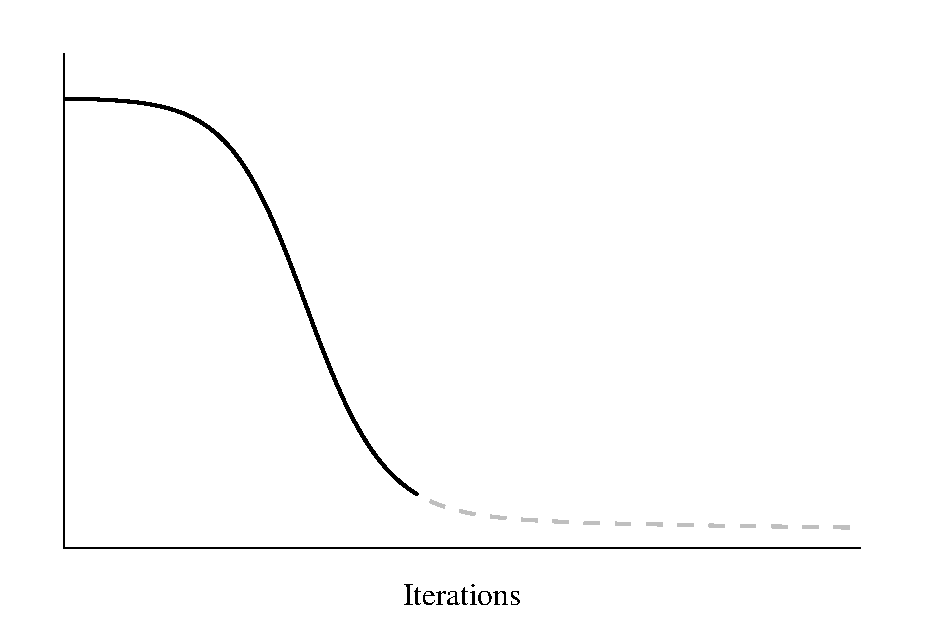
\includegraphics[width=5cm]{convergence2.eps}};
  \node[rotate=90] at (15.5,3) { $\left| \mathbb{E} \! \left[ f \right] - \hat{f} \right|$ };
\end{tikzpicture}
}
\subfigure[]{
\begin{tikzpicture}[scale=0.25, thick]
  \draw[-,color=white] (-12, 0) to (12, 0);
  
  \begin{scope}
  \clip (-12, -10) rectangle (12, 10);
  \foreach \i in {0, 0.05,..., 1} {
    \draw[line width={30 * \i}, opacity={exp(-8 * \i)}, dark] 
      (-10, 0) .. controls (-10, 15) and (-5, 5) .. (0, 5)
      .. controls (5, 5) and (10, 8) .. (10, 0)
      .. controls (10, -8) and (5, -3) .. (0, -3)
      .. controls (-5, -3) and (-10, -5) .. (-10, 0);
  }
  
  %\fill[color=dark] (-11, -8) circle (7pt);  
  %\fill[color=light] (-11, -8) circle (5pt);
  
  \fill[color=dark] (-10, -6.5) circle (7pt);  
  \fill[color=light] (-10, -6.5) circle (5pt);
  
  \fill[color=dark] (-9, -6.75) circle (7pt);  
  \fill[color=light] (-9, -6.75) circle (5pt);
  
  \fill[color=dark] (-8.25, -5) circle (7pt);  
  \fill[color=light] (-8.25, -5) circle (5pt);
  
  \fill[color=dark] (-7.5, -4) circle (7pt);  
  \fill[color=light] (-7.5, -4) circle (5pt);
  
  \fill[color=dark] (-7, -3.5) circle (7pt);  
  \fill[color=light] (-7, -3.5) circle (5pt);
  
  \fill[color=dark] (-6.5, -3.6) circle (7pt);  
  \fill[color=light] (-6.5, -3.6) circle (5pt);  
  
  \fill[color=dark] (-6, -3) circle (7pt);  
  \fill[color=light] (-6, -3) circle (5pt);
  
  \fill[color=dark] (-5.5, -3.5) circle (7pt);  
  \fill[color=light] (-5.5, -3.5) circle (5pt);
  
  \fill[color=dark] (-5, -3.75) circle (7pt);  
  \fill[color=light] (-5, -3.75) circle (5pt);
  
  \fill[color=dark] (-4.75, -3.25) circle (7pt);  
  \fill[color=light] (-4.75, -3.25) circle (5pt);
  
  \fill[color=dark] (-5, -3.5) circle (7pt);  
  \fill[color=light] (-5, -3.5) circle (5pt);  
  
  \fill[color=dark] (-4, -3.8) circle (7pt);  
  \fill[color=light] (-4, -3.8) circle (5pt);
  
  \fill[color=dark] (-3, -3.5) circle (7pt);  
  \fill[color=light] (-3, -3.5) circle (5pt);
  
  \fill[color=dark] (-2.8, -3) circle (7pt);  
  \fill[color=light] (-2.8, -3) circle (5pt);
  
  \fill[color=dark] (-2.9, -3.3) circle (7pt);  
  \fill[color=light] (-2.9, -3.3) circle (5pt);  
  
  \fill[color=dark] (-2, -3.5) circle (7pt);  
  \fill[color=light] (-2, -3.5) circle (5pt);
  
  \fill[color=dark] (-1.25, -3) circle (7pt);  
  \fill[color=light] (-1.25, -3) circle (5pt);
  
  \fill[color=dark] (-0.5, -2.75) circle (7pt);  
  \fill[color=light] (-0.5, -2.75) circle (5pt);
  
  \fill[color=dark] (-0.3, -3) circle (7pt);  
  \fill[color=light] (-0.3, -3) circle (5pt);  
  
  \fill[color=dark] (0.1, -2.75) circle (7pt);  
  \fill[color=light] (0.1, -2.75) circle (5pt);
  
  \fill[color=dark] (0.15, -3.1) circle (7pt);  
  \fill[color=light] (0.15, -3.1) circle (5pt);  
  
  \fill[color=dark] (0.4, -3.4) circle (7pt);  
  \fill[color=light] (0.4, -3.4) circle (5pt);
  
  \fill[color=dark] (1.1, -3.25) circle (7pt);  
  \fill[color=light] (1.1, -3.25) circle (5pt);
  
  \fill[color=dark] (2.7, -3.45) circle (7pt);  
  \fill[color=light] (2.7, -3.45) circle (5pt);
  
  \fill[color=dark] (2.9, -3.2) circle (7pt);  
  \fill[color=light] (2.9, -3.2) circle (5pt);
  
  \fill[color=dark] (3.1, -3.7) circle (7pt);  
  \fill[color=light] (3.1, -3.7) circle (5pt);
  
  \fill[color=dark] (4.2, -3.9) circle (7pt);  
  \fill[color=light] (4.2, -3.9) circle (5pt);
  
  \fill[color=dark] (4, -4.1) circle (7pt);  
  \fill[color=light] (4, -4.1) circle (5pt);
  
  \fill[color=dark] (5, -4) circle (7pt);  
  \fill[color=light] (5, -4) circle (5pt);
  
  \fill[color=dark] (5.8, -4.3) circle (7pt);  
  \fill[color=light] (5.8, -4.3) circle (5pt);
  
  \fill[color=dark] (6.5, -4.8) circle (7pt);  
  \fill[color=light] (6.5, -4.8) circle (5pt);
  
  \fill[color=dark] (6.8, -4.5) circle (7pt);  
  \fill[color=light] (6.8, -4.5) circle (5pt);
  
  \fill[color=dark] (7, -4.6) circle (7pt);  
  \fill[color=light] (7, -4.6) circle (5pt);
  
  \fill[color=dark] (6.8, -4.7) circle (7pt);  
  \fill[color=light] (6.8, -4.7) circle (5pt);
  
  \fill[color=dark] (7.75, -4.2) circle (7pt);  
  \fill[color=light] (7.75, -4.2) circle (5pt);
  
  \fill[color=dark] (8.5, -4.25) circle (7pt);  
  \fill[color=light] (8.5, -4.25) circle (5pt);
  
  \fill[color=dark] (8.6, -4.75) circle (7pt);  
  \fill[color=light] (8.6, -4.75) circle (5pt);
  
  \fill[color=dark] (8.8, -4.5) circle (7pt);  
  \fill[color=light] (8.8, -4.5) circle (5pt);
  
  \fill[color=dark] (9.25, -3.5) circle (7pt);  
  \fill[color=light] (9.25, -3.5) circle (5pt);
  
  \fill[color=dark] (9.65, -2.75) circle (7pt);  
  \fill[color=light] (9.65, -2.75) circle (5pt);
  
  \fill[color=dark] (9.5, -2) circle (7pt);  
  \fill[color=light] (9.5, -2) circle (5pt);

  \fill[color=dark] (9.8, -3) circle (7pt);  
  \fill[color=light] (9.8, -3) circle (5pt);
  
  \fill[color=dark] (9.85, -0.8) circle (7pt);  
  \fill[color=light] (9.85, -0.8) circle (5pt);
  
  \fill[color=dark] (10.1, -0.4) circle (7pt);  
  \fill[color=light] (10.1, -0.4) circle (5pt);

  \fill[color=dark] (10.25, 0.3) circle (7pt);  
  \fill[color=light] (10.25, 0.3) circle (5pt);
  
  \fill[color=dark] (10, 0.7) circle (7pt);  
  \fill[color=light] (10, 0.7) circle (5pt);
  
  \fill[color=dark] (9.7, 0.9) circle (7pt);  
  \fill[color=light] (9.7, 0.9) circle (5pt);
  
  \fill[color=dark] (10.3, 1.4) circle (7pt);  
  \fill[color=light] (10.3, 1.4) circle (5pt);
  
  \fill[color=dark] (9.8, 2.25) circle (7pt);  
  \fill[color=light] (9.8, 2.25) circle (5pt);
  
  \fill[color=dark] (10, 2.5) circle (7pt);  
  \fill[color=light] (10, 2.5) circle (5pt);
  
  \fill[color=dark] (10, 3) circle (7pt);  
  \fill[color=light] (10, 3) circle (5pt);
  
  \fill[color=dark] (9.6, 3.75) circle (7pt);  
  \fill[color=light] (9.6, 3.75) circle (5pt);
  
  \fill[color=dark] (9.1, 4.4) circle (7pt);  
  \fill[color=light] (9.1, 4.4) circle (5pt);
  
  \fill[color=dark] (9.1, 4.1) circle (7pt);  
  \fill[color=light] (9.1, 4.1) circle (5pt);
  
  \fill[color=dark] (8.5, 4.75) circle (7pt);  
  \fill[color=light] (8.5, 4.75) circle (5pt);
  
  \fill[color=dark] (8.1, 5.75) circle (7pt);  
  \fill[color=light] (8.1, 5.75) circle (5pt);
  
  \fill[color=dark] (7.7, 5.2) circle (7pt);  
  \fill[color=light] (7.7, 5.2) circle (5pt);
  
  \fill[color=dark] (7.3, 5.3) circle (7pt);  
  \fill[color=light] (7.3, 5.3) circle (5pt);
  
  \fill[color=dark] (6.6, 5.8) circle (7pt);  
  \fill[color=light] (6.6, 5.8) circle (5pt);
  
  \fill[color=dark] (6, 6) circle (7pt);  
  \fill[color=light] (6, 6) circle (5pt);
  
  \fill[color=dark] (5.25, 5.45) circle (7pt);  
  \fill[color=light] (5.25, 5.45) circle (5pt);
  
  \fill[color=dark] (4.75, 5.75) circle (7pt);  
  \fill[color=light] (4.75, 5.75) circle (5pt);
  
  \fill[color=dark] (3.5, 5.28) circle (7pt);  
  \fill[color=light] (3.5, 5.28) circle (5pt);
  
  \fill[color=dark] (5, 5.65) circle (7pt);  
  \fill[color=light] (5, 5.65) circle (5pt);
  
  \fill[color=dark] (3, 5.5) circle (7pt);  
  \fill[color=light] (3, 5.5) circle (5pt);
  
  \fill[color=dark] (2.75, 5.3) circle (7pt);  
  \fill[color=light] (2.75, 5.3) circle (5pt);
  
  \fill[color=dark] (2.25, 4.8) circle (7pt);  
  \fill[color=light] (2.25, 4.8) circle (5pt);
  
  \fill[color=dark] (2, 5.2) circle (7pt);  
  \fill[color=light] (2, 5.2) circle (5pt);
  
  \fill[color=dark] (1.75, 4.9) circle (7pt);  
  \fill[color=light] (1.75, 4.9) circle (5pt);
  
  \fill[color=dark] (1.5, 5.1) circle (7pt);  
  \fill[color=light] (1.5, 5.1) circle (5pt);
  
  \fill[color=dark] (0.8, 5.2) circle (7pt);  
  \fill[color=light] (0.8, 5.2) circle (5pt);
 
  \fill[color=dark] (0, 4.7) circle (7pt);  
  \fill[color=light] (0, 4.7) circle (5pt);
  
  \fill[color=dark] (-0.6, 5) circle (7pt);  
  \fill[color=light] (-0.6, 5) circle (5pt);
  
  \fill[color=dark] (-1.25, 5.2) circle (7pt);  
  \fill[color=light] (-1.25, 5.2) circle (5pt);
  
  \fill[color=dark] (-1.55, 5.4) circle (7pt);  
  \fill[color=light] (-1.55, 5.4) circle (5pt);
  
  \fill[color=dark] (-1.85, 5) circle (7pt);  
  \fill[color=light] (-1.85, 5) circle (5pt);
  
  \fill[color=dark] (-2.75, 5.5) circle (7pt);  
  \fill[color=light] (-2.75, 5.5) circle (5pt);
  
  \fill[color=dark] (-3.5, 6.6) circle (7pt);  
  \fill[color=light] (-3.5, 6.6) circle (5pt);
  
  \fill[color=dark] (-4.25, 6.5) circle (7pt);  
  \fill[color=light] (-4.25, 6.5) circle (5pt);
  
  \fill[color=dark] (-4.9, 7.2) circle (7pt);  
  \fill[color=light] (-4.9, 7.2) circle (5pt);
  
  \fill[color=dark] (-5.2, 7) circle (7pt);  
  \fill[color=light] (-5.2, 7) circle (5pt);
  
  \fill[color=dark] (-5.75, 7.4) circle (7pt);  
  \fill[color=light] (-5.75, 7.4) circle (5pt);
  
  \fill[color=dark] (-6, 7.9) circle (7pt);  
  \fill[color=light] (-6, 7.9) circle (5pt);
  
  \fill[color=dark] (-6.25, 7.8) circle (7pt);  
  \fill[color=light] (-6.25, 7.8) circle (5pt);
  
  \fill[color=dark] (-6.5, 7.5) circle (7pt);  
  \fill[color=light] (-6.5, 7.5) circle (5pt);
  
  \fill[color=dark] (-6.75, 8) circle (7pt);  
  \fill[color=light] (-6.75, 8) circle (5pt);
  
  \fill[color=dark] (-7.5, 8.5) circle (7pt);  
  \fill[color=light] (-7.5, 8.5) circle (5pt);
  
  \fill[color=dark] (-8.25, 8) circle (7pt);  
  \fill[color=light] (-8.25, 8) circle (5pt);
  
  \fill[color=dark] (-8.65, 7.8) circle (7pt);  
  \fill[color=light] (-8.65, 7.8) circle (5pt);
  
  \fill[color=dark] (-8.4, 7.7) circle (7pt);  
  \fill[color=light] (-8.4, 7.7) circle (5pt);
  
  \fill[color=dark] (-9.2, 7) circle (7pt);  
  \fill[color=light] (-9.2, 7) circle (5pt);
  
  \fill[color=dark] (-9.5, 6.75) circle (7pt);  
  \fill[color=light] (-9.5, 6.75) circle (5pt);
  
  \fill[color=dark] (-10, 6) circle (7pt);  
  \fill[color=light] (-10, 6) circle (5pt);
  
  \fill[color=dark] (-9.7, 5.3) circle (7pt);  
  \fill[color=light] (-9.7, 5.3) circle (5pt);
  
  \fill[color=dark] (-9.6, 5) circle (7pt);  
  \fill[color=light] (-9.6, 5) circle (5pt);
  
  \fill[color=dark] (-9.9, 4.75) circle (7pt);  
  \fill[color=light] (-9.9, 4.75) circle (5pt);
  
  \fill[color=dark] (-10.1, 4) circle (7pt);  
  \fill[color=light] (-10.1, 4) circle (5pt);
  
  \fill[color=dark] (-9.7, 3.5) circle (7pt);  
  \fill[color=light] (-9.7, 3.5) circle (5pt);
  
  \fill[color=dark] (-9.8, 3) circle (7pt);  
  \fill[color=light] (-9.8, 3) circle (5pt);
  
  \fill[color=dark] (-10, 2.2) circle (7pt);  
  \fill[color=light] (-10, 2.2) circle (5pt);  
  
  \fill[color=dark] (-10.25, 1.9) circle (7pt);  
  \fill[color=light] (-10.25, 1.9) circle (5pt);  
  
  \fill[color=dark] (-9.7, 1.8) circle (7pt);  
  \fill[color=light] (-9.7, 1.8) circle (5pt);  
  
  \fill[color=dark] (-10.2, 1.4) circle (7pt);  
  \fill[color=light] (-10.2, 1.4) circle (5pt);  
  
  \fill[color=dark] (-9.8, 0.7) circle (7pt);  
  \fill[color=light] (-9.8, 0.7) circle (5pt);  
  
  \fill[color=dark] (-10.2, 0.1) circle (7pt);  
  \fill[color=light] (-10.2, 0.1) circle (5pt);  
  
  \fill[color=dark] (-9.9, -0.1) circle (7pt);  
  \fill[color=light] (-9.9, -0.1) circle (5pt);  
  
  \fill[color=dark] (-10, -0.9) circle (7pt);  
  \fill[color=light] (-10, -0.9) circle (5pt);  
  
  \fill[color=dark] (-9.6, -1.5) circle (7pt);  
  \fill[color=light] (-9.6, -1.5) circle (5pt);  
  
  \fill[color=dark] (-9.5, -1.8) circle (7pt);  
  \fill[color=light] (-9.5, -1.8) circle (5pt);  
  
  \fill[color=dark] (-9.7, -2.1) circle (7pt);  
  \fill[color=light] (-9.7, -2.1) circle (5pt);  
  
  \fill[color=dark] (-9.3, -2.8) circle (7pt);  
  \fill[color=light] (-9.3, -2.8) circle (5pt);  
  
  \fill[color=dark] (-8.3, -3) circle (7pt);  
  \fill[color=light] (-8.3, -3) circle (5pt);  
  
  \fill[color=dark] (-7.8, -3.4) circle (7pt);  
  \fill[color=light] (-7.8, -3.4) circle (5pt);  
  
  \fill[color=dark] (-7.6, -3) circle (7pt);  
  \fill[color=light] (-7.6, -3) circle (5pt);   
  
  \end{scope}
  
  \draw[-,color=white] (14, 0) to (38, 0);  
  \node[] at (28,3) {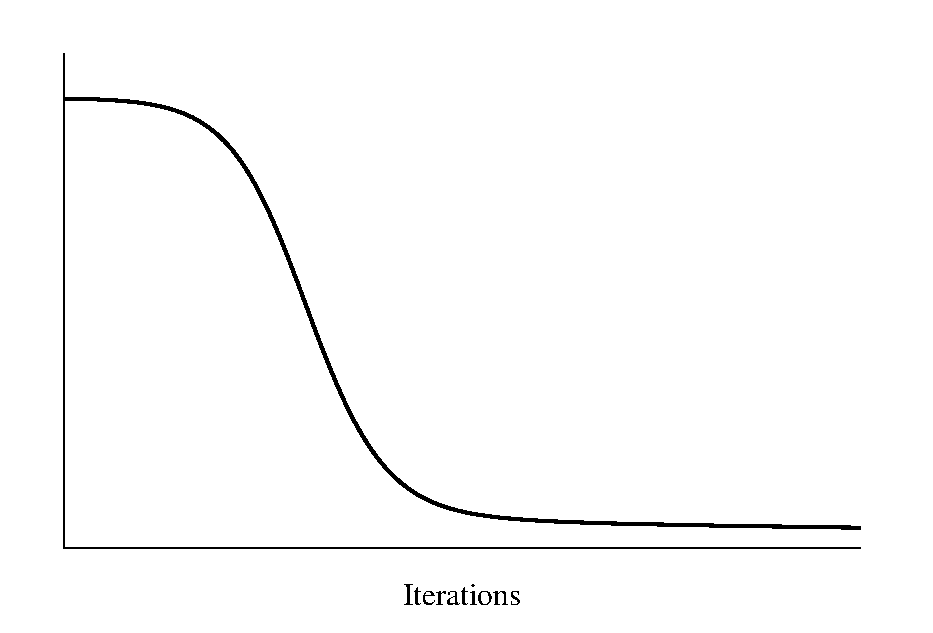
\includegraphics[width=5cm]{convergence3.eps}};
  \node[rotate=90] at (15.5,3) { $\left| \mathbb{E} \! \left[ f \right] - \hat{f} \right|$ };
\end{tikzpicture}
}
\caption{Under ideal circumstances, a Markov chain explores 
the target distribution in three phases.  (a) First the Markov
chain convergences to the typical set and estimators suffer
from initial but ultimately transient biases. (b) Once the Markov 
chain finds the typical set and makes it first sojourn through it,
this initial bias rapidly vanishes and the estimators become
much more accurate.  (c) As the Markov chain continues it
explores more details of the typical set and gradually improves
estimator precision.}
\label{fig:ideal_mcmc}
\end{figure*}

Once the Markov chain has entered into this third phase
the Markov chain Monte Carlo estimators satisfy a Central 
Limit Theorem
%
\begin{equation*}
\hat{f}_{N}^{\mathrm{MCMC}} \sim 
\mathcal{N} \! \left( \EE_{\PP} [ f ],
\mathrm{MCMCSE} \right),
\end{equation*}
%
where the \emph{Markov Chain Monte Carlo Standard Error} is 
given by
%
\begin{equation*}
\mathrm{MCMCSE} \equiv \sqrt{ \frac{ \mathrm{Var} [ f ] }{\mathrm{ESS} } }.
\end{equation*}
%
Here the \emph{effective sample size} is defined as
%
\begin{equation*}
\mathrm{ESS} = 
\frac{N}
{ 1 + 2 \sum_{l = 1}^{\infty} \rho_{l} },
\end{equation*}
%
where $\rho_{l}$ is the lag-$l$ autocorrelation of $f$ over the history
of the Markov chain.  As in the Importance Sampling Central Limit 
Theorem, the effective sample size quantifies the number of exact 
samples necessary to give an equivalent estimator precision and 
hence the effective number of exact samples ``contained'' in the 
Markov chain.  We can also interpret the effective sample size as 
the total number of sojourns the Markov chain has made through 
the typical set.

Because the states of the Markov chain during the initial convergence
phase mostly bias Markov chain Monte Carlo estimators, we can
achieve more precise estimators more quickly by using samples
generated only once the Markov chain has begun to explore the
typical set.  Consequently typical practice is to throw away some
number of initial samples before computing Markov chain Monte
Carlo estimators.

\subsubsection{Markov Chain Monte Carlo Under Less-Than-Ideal Conditions}

Under ideal conditions Markov chain Monte Carlo behaves
very similarly to Monte Carlo, only with a loss of efficiency due
to the correlation in the samples.  When the target distribution
exhibits more pathological behavior, however, Monte Carlo
continues to perform well while Markov chain Monte Carlo
begins to fail in spectacular fashion.

Consider, for example, a target probability distribution where
the typical set pinches into a region of high curvature
(Figure \ref{fig:pathological_typical_set}).  Most Markov
transitions do not have the resolution to maneuver into
these tight regions and the resulting Markov chains simply
ignore them, biasing subsequent Markov chain Monte Carlo
estimators.  It's as if there are thin but deep cracks hiding 
a significant amount of probability that the Markov chains 
pass right over and miss entirely.

\begin{figure*}
\centering
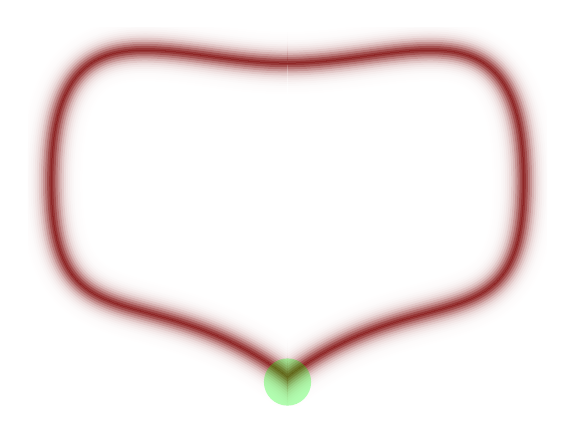
\begin{tikzpicture}[scale=0.3, thick]

\foreach \i in {0, 0.05,..., 1} {
  \begin{scope}
    \clip (-0.005, -9.5) rectangle (11, 6.5);
    \draw[line width={30 * \i}, opacity={exp(-8 * \i)}, dark] 
    (0, 5) .. controls (5, 5) and (10, 8) .. (10, 0)
             .. controls (10, -8) and (5, -3) .. (-2, -10);
  \end{scope}
  
  \begin{scope}
    \clip (0.005, -9.5) rectangle (-11, 6.5);
    \draw[line width={30 * \i}, opacity={exp(-8 * \i)}, dark] 
    (0, 5) .. controls (-5, 5) and (-10, 8) .. (-10, 0)
             .. controls (-10, -8) and (-5, -3) .. (2, -10);
  \end{scope}
}  
\fill[opacity=0.3, green] (0, -8.5) circle (1);
\end{tikzpicture}
%
\caption{Markov chains typically have trouble exploring regions 
of the typical set with large curvature (green), which induces
bias in Markov chain Monte Carlo estimators and spoils useful
behavior such as Central Limit Theorems.}
\label{fig:pathological_typical_set}
\end{figure*}

Because Markov chains have to recover the exact expectations
asymptotically, they have to somehow compensate for not being
able to explore these regions.  Typically the Markov chain
accomplishes this by getting stuck near the boundary of the
pathological region: as it hovers the estimators are drawn down 
as if the Markov chain were exploring the pathological region.
Eventually the Markov chain escapes to explore the rest of the
typical set and the estimator bias begins to increase again
(Figure \ref{fig:pathological exploration}).  

\begin{figure*}
\centering
\subfigure[]{
\begin{tikzpicture}[scale=0.25, thick]
  \draw[-,color=white] (-12, 0) to (12, 0);
  
  \foreach \i in {0, 0.05,..., 1} {
    \begin{scope}
      \clip (-0.005, -9.5) rectangle (11, 6.5);
      \draw[line width={30 * \i}, opacity={exp(-8 * \i)}, dark] 
      (0, 5) .. controls (5, 5) and (10, 8) .. (10, 0)
               .. controls (10, -8) and (5, -3) .. (-2, -10);
    \end{scope}
  
    \begin{scope}
      \clip (0.005, -9.5) rectangle (-11, 6.5);
      \draw[line width={30 * \i}, opacity={exp(-8 * \i)}, dark] 
      (0, 5) .. controls (-5, 5) and (-10, 8) .. (-10, 0)
               .. controls (-10, -8) and (-5, -3) .. (2, -10);
    \end{scope}
  }  
  \fill[opacity=0.3, green] (0, -8.5) circle (1);
  
  \fill[color=dark] (-8, 5.5) circle (7pt);  
  \fill[color=light] (-8, 5.5) circle (5pt);  
  
  \fill[color=dark] (-9, 4.75) circle (7pt);  
  \fill[color=light] (-9, 4.75) circle (5pt);  

  \fill[color=dark] (-8.7, 4.6) circle (7pt);  
  \fill[color=light] (-8.7, 4.6) circle (5pt); 
  
  \fill[color=dark] (-9.1, 4.5) circle (7pt);  
  \fill[color=light] (-9.1, 4.5) circle (5pt);  
  
  \fill[color=dark] (-9.2, 3.5) circle (7pt);  
  \fill[color=light] (-9.2, 3.5) circle (5pt);   
  
  \fill[color=dark] (-9.9, 3) circle (7pt);  
  \fill[color=light] (-9.9, 3) circle (5pt); 
  
  \fill[color=dark] (-10.1, 2.15) circle (7pt);  
  \fill[color=light] (-10.1, 2.15) circle (5pt);   
  
  \fill[color=dark] (-9.6, 1.5) circle (7pt);  
  \fill[color=light] (-9.6, 1.5) circle (5pt);   
  
  \fill[color=dark] (-9.75, 1) circle (7pt);  
  \fill[color=light] (-9.75, 1) circle (5pt); 
  
  \fill[color=dark] (-10.2, 0.25) circle (7pt);  
  \fill[color=light] (-10.2, 0.25) circle (5pt); 
  
  \fill[color=dark] (-9.8, 0) circle (7pt);  
  \fill[color=light] (-9.8, 0) circle (5pt); 
  
  \fill[color=dark] (-10, -0.5) circle (7pt);  
  \fill[color=light] (-10, -0.5) circle (5pt); 
  
  \fill[color=dark] (-9.75, -2) circle (7pt);  
  \fill[color=light] (-9.75, -2) circle (5pt);
  
  \fill[color=dark] (-9.9, -3) circle (7pt);  
  \fill[color=light] (-9.9, -3) circle (5pt);  
  
  \fill[color=dark] (-9.25, -3.5) circle (7pt);  
  \fill[color=light] (-9.25, -3.5) circle (5pt);   
  
  \fill[color=dark] (-9, -4.25) circle (7pt);  
  \fill[color=light] (-9, -4.25) circle (5pt);   
     
  \fill[color=dark] (-8, -4.5) circle (7pt);  
  \fill[color=light] (-8, -4.5) circle (5pt);  
  
  \fill[color=dark] (-8.25, -4.75) circle (7pt);  
  \fill[color=light] (-8.25, -4.75) circle (5pt);  

  \fill[color=dark] (-7.75, -5) circle (7pt);  
  \fill[color=light] (-7.75, -5) circle (5pt);  
  
  \fill[color=dark] (-6.5, -5.5) circle (7pt);  
  \fill[color=light] (-6.5, -5.5) circle (5pt);  
  
  \fill[color=dark] (-5.75, -5.25) circle (7pt);  
  \fill[color=light] (-5.75, -5.25) circle (5pt);  
  
  \fill[color=dark] (-5, -6) circle (7pt);  
  \fill[color=light] (-5, -6) circle (5pt);  
  
  \fill[color=dark] (-4.75, -6.25) circle (7pt);  
  \fill[color=light] (-4.75, -6.25) circle (5pt);  
  
  \fill[color=dark] (-3.8, -6) circle (7pt);  
  \fill[color=light] (-3.8, -6) circle (5pt);  
  
  \fill[color=dark] (-3.25, -6.5) circle (7pt);  
  \fill[color=light] (-3.25, -6.5) circle (5pt); 
  
  \fill[color=dark] (-2.75, -6.75) circle (7pt);  
  \fill[color=light] (-2.75, -6.75) circle (5pt);   
  
  \fill[color=dark] (-2, -7.5) circle (7pt);  
  \fill[color=light] (-2, -7.5) circle (5pt); 
  
  \fill[color=dark] (-1.75, -6.8) circle (7pt);  
  \fill[color=light] (-1.75, -6.8) circle (5pt);  
  
  \fill[color=dark] (-1.5, -7.2) circle (7pt);  
  \fill[color=light] (-1.5, -7.2) circle (5pt); 

  \draw[-,color=white] (14, 0) to (38, 0);  
  \node[] at (28,-2) {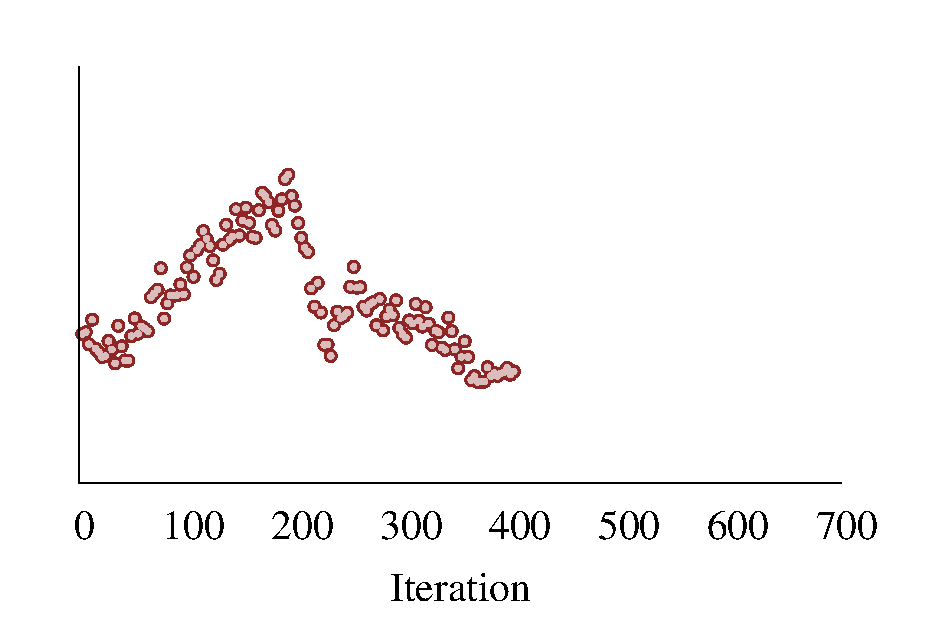
\includegraphics[width=6cm]{funnel_trace1.eps}};
\end{tikzpicture}
}
\subfigure[]{
\begin{tikzpicture}[scale=0.25, thick]
  \draw[-,color=white] (-12, 0) to (12, 0);
  
  \foreach \i in {0, 0.05,..., 1} {
    \begin{scope}
      \clip (-0.005, -9.5) rectangle (11, 6.5);
      \draw[line width={30 * \i}, opacity={exp(-8 * \i)}, dark] 
      (0, 5) .. controls (5, 5) and (10, 8) .. (10, 0)
               .. controls (10, -8) and (5, -3) .. (-2, -10);
    \end{scope}
  
    \begin{scope}
      \clip (0.005, -9.5) rectangle (-11, 6.5);
      \draw[line width={30 * \i}, opacity={exp(-8 * \i)}, dark] 
      (0, 5) .. controls (-5, 5) and (-10, 8) .. (-10, 0)
               .. controls (-10, -8) and (-5, -3) .. (2, -10);
    \end{scope}
  }  
  \fill[opacity=0.3, green] (0, -8.5) circle (1);
  
  \fill[color=dark] (-8, 5.5) circle (7pt);  
  \fill[color=light] (-8, 5.5) circle (5pt);  
  
  \fill[color=dark] (-9, 4.75) circle (7pt);  
  \fill[color=light] (-9, 4.75) circle (5pt);  

  \fill[color=dark] (-8.7, 4.6) circle (7pt);  
  \fill[color=light] (-8.7, 4.6) circle (5pt); 
  
  \fill[color=dark] (-9.1, 4.5) circle (7pt);  
  \fill[color=light] (-9.1, 4.5) circle (5pt);  
  
  \fill[color=dark] (-9.2, 3.5) circle (7pt);  
  \fill[color=light] (-9.2, 3.5) circle (5pt);   
  
  \fill[color=dark] (-9.9, 3) circle (7pt);  
  \fill[color=light] (-9.9, 3) circle (5pt); 
  
  \fill[color=dark] (-10.1, 2.15) circle (7pt);  
  \fill[color=light] (-10.1, 2.15) circle (5pt);   
  
  \fill[color=dark] (-9.6, 1.5) circle (7pt);  
  \fill[color=light] (-9.6, 1.5) circle (5pt);   
  
  \fill[color=dark] (-9.75, 1) circle (7pt);  
  \fill[color=light] (-9.75, 1) circle (5pt); 
  
  \fill[color=dark] (-10.2, 0.25) circle (7pt);  
  \fill[color=light] (-10.2, 0.25) circle (5pt); 
  
  \fill[color=dark] (-9.8, 0) circle (7pt);  
  \fill[color=light] (-9.8, 0) circle (5pt); 
  
  \fill[color=dark] (-10, -0.5) circle (7pt);  
  \fill[color=light] (-10, -0.5) circle (5pt); 
  
  \fill[color=dark] (-9.75, -2) circle (7pt);  
  \fill[color=light] (-9.75, -2) circle (5pt);
  
  \fill[color=dark] (-9.9, -3) circle (7pt);  
  \fill[color=light] (-9.9, -3) circle (5pt);  
  
  \fill[color=dark] (-9.25, -3.5) circle (7pt);  
  \fill[color=light] (-9.25, -3.5) circle (5pt);   
  
  \fill[color=dark] (-9, -4.25) circle (7pt);  
  \fill[color=light] (-9, -4.25) circle (5pt);   
     
  \fill[color=dark] (-8, -4.5) circle (7pt);  
  \fill[color=light] (-8, -4.5) circle (5pt);  
  
  \fill[color=dark] (-8.25, -4.75) circle (7pt);  
  \fill[color=light] (-8.25, -4.75) circle (5pt);  

  \fill[color=dark] (-7.75, -5) circle (7pt);  
  \fill[color=light] (-7.75, -5) circle (5pt);  
  
  \fill[color=dark] (-6.5, -5.5) circle (7pt);  
  \fill[color=light] (-6.5, -5.5) circle (5pt);  
  
  \fill[color=dark] (-5.75, -5.25) circle (7pt);  
  \fill[color=light] (-5.75, -5.25) circle (5pt);  
  
  \fill[color=dark] (-5, -6) circle (7pt);  
  \fill[color=light] (-5, -6) circle (5pt);  
  
  \fill[color=dark] (-4.75, -6.25) circle (7pt);  
  \fill[color=light] (-4.75, -6.25) circle (5pt);  
  
  \fill[color=dark] (-3.8, -6) circle (7pt);  
  \fill[color=light] (-3.8, -6) circle (5pt);  
  
  \fill[color=dark] (-3.25, -6.5) circle (7pt);  
  \fill[color=light] (-3.25, -6.5) circle (5pt); 
  
  \fill[color=dark] (-2.75, -6.75) circle (7pt);  
  \fill[color=light] (-2.75, -6.75) circle (5pt);   
  
  \fill[color=dark] (-2, -7.5) circle (7pt);  
  \fill[color=light] (-2, -7.5) circle (5pt); 
  
  \fill[color=dark] (-1.75, -6.8) circle (7pt);  
  \fill[color=light] (-1.75, -6.8) circle (5pt);  
  
  \fill[color=dark] (-1.5, -7.2) circle (7pt);  
  \fill[color=light] (-1.5, -7.2) circle (5pt); 
  
  \fill[color=dark] (-0.5, -7.5) circle (7pt);  
  \fill[color=light] (-0.5, -7.5) circle (5pt);
  
  \fill[color=dark] (0, -7.6) circle (7pt);  
  \fill[color=light] (0, -7.6) circle (5pt);  
  
  \fill[color=dark] (1, -7.7) circle (7pt);  
  \fill[color=light] (1, -7.7) circle (5pt);  

  \draw[-,color=white] (14, 0) to (38, 0);  
  \node[] at (28,-2) {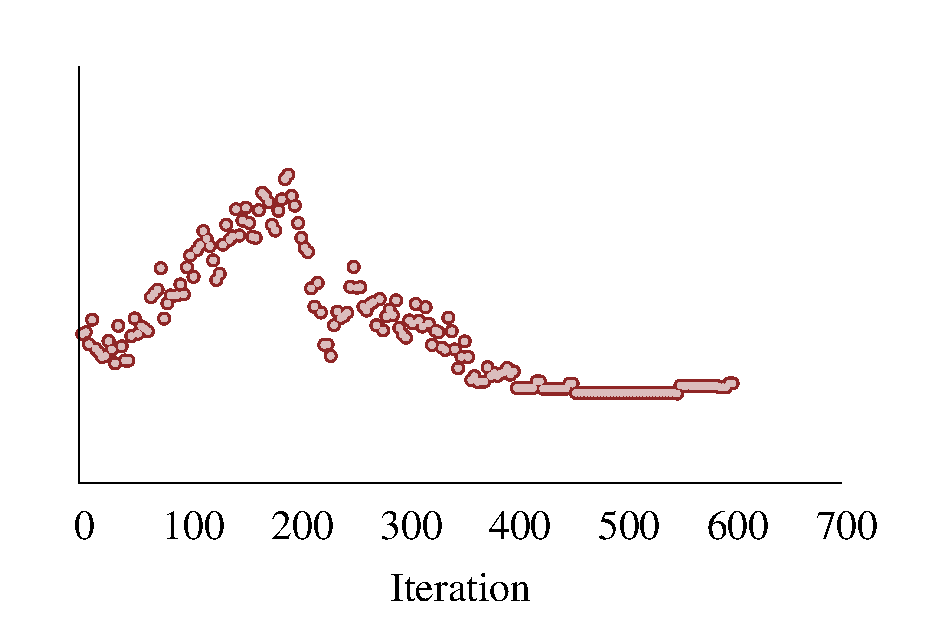
\includegraphics[width=6cm]{funnel_trace2.eps}};
\end{tikzpicture}
}
\subfigure[]{
\begin{tikzpicture}[scale=0.25, thick]
  \draw[-,color=white] (-12, 0) to (12, 0);
  
  \foreach \i in {0, 0.05,..., 1} {
    \begin{scope}
      \clip (-0.005, -9.5) rectangle (11, 6.5);
      \draw[line width={30 * \i}, opacity={exp(-8 * \i)}, dark] 
      (0, 5) .. controls (5, 5) and (10, 8) .. (10, 0)
               .. controls (10, -8) and (5, -3) .. (-2, -10);
    \end{scope}
  
    \begin{scope}
      \clip (0.005, -9.5) rectangle (-11, 6.5);
      \draw[line width={30 * \i}, opacity={exp(-8 * \i)}, dark] 
      (0, 5) .. controls (-5, 5) and (-10, 8) .. (-10, 0)
               .. controls (-10, -8) and (-5, -3) .. (2, -10);
    \end{scope}
  }  
  \fill[opacity=0.3, green] (0, -8.5) circle (1);
  
  \fill[color=dark] (-8, 5.5) circle (7pt);  
  \fill[color=light] (-8, 5.5) circle (5pt);  
  
  \fill[color=dark] (-9, 4.75) circle (7pt);  
  \fill[color=light] (-9, 4.75) circle (5pt);  

  \fill[color=dark] (-8.7, 4.6) circle (7pt);  
  \fill[color=light] (-8.7, 4.6) circle (5pt); 
  
  \fill[color=dark] (-9.1, 4.5) circle (7pt);  
  \fill[color=light] (-9.1, 4.5) circle (5pt);  
  
  \fill[color=dark] (-9.2, 3.5) circle (7pt);  
  \fill[color=light] (-9.2, 3.5) circle (5pt);   
  
  \fill[color=dark] (-9.9, 3) circle (7pt);  
  \fill[color=light] (-9.9, 3) circle (5pt); 
  
  \fill[color=dark] (-10.1, 2.15) circle (7pt);  
  \fill[color=light] (-10.1, 2.15) circle (5pt);   
  
  \fill[color=dark] (-9.6, 1.5) circle (7pt);  
  \fill[color=light] (-9.6, 1.5) circle (5pt);   
  
  \fill[color=dark] (-9.75, 1) circle (7pt);  
  \fill[color=light] (-9.75, 1) circle (5pt); 
  
  \fill[color=dark] (-10.2, 0.25) circle (7pt);  
  \fill[color=light] (-10.2, 0.25) circle (5pt); 
  
  \fill[color=dark] (-9.8, 0) circle (7pt);  
  \fill[color=light] (-9.8, 0) circle (5pt); 
  
  \fill[color=dark] (-10, -0.5) circle (7pt);  
  \fill[color=light] (-10, -0.5) circle (5pt); 
  
  \fill[color=dark] (-9.75, -2) circle (7pt);  
  \fill[color=light] (-9.75, -2) circle (5pt);
  
  \fill[color=dark] (-9.9, -3) circle (7pt);  
  \fill[color=light] (-9.9, -3) circle (5pt);  
  
  \fill[color=dark] (-9.25, -3.5) circle (7pt);  
  \fill[color=light] (-9.25, -3.5) circle (5pt);   
  
  \fill[color=dark] (-9, -4.25) circle (7pt);  
  \fill[color=light] (-9, -4.25) circle (5pt);   
     
  \fill[color=dark] (-8, -4.5) circle (7pt);  
  \fill[color=light] (-8, -4.5) circle (5pt);  
  
  \fill[color=dark] (-8.25, -4.75) circle (7pt);  
  \fill[color=light] (-8.25, -4.75) circle (5pt);  

  \fill[color=dark] (-7.75, -5) circle (7pt);  
  \fill[color=light] (-7.75, -5) circle (5pt);  
  
  \fill[color=dark] (-6.5, -5.5) circle (7pt);  
  \fill[color=light] (-6.5, -5.5) circle (5pt);  
  
  \fill[color=dark] (-5.75, -5.25) circle (7pt);  
  \fill[color=light] (-5.75, -5.25) circle (5pt);  
  
  \fill[color=dark] (-5, -6) circle (7pt);  
  \fill[color=light] (-5, -6) circle (5pt);  
  
  \fill[color=dark] (-4.75, -6.25) circle (7pt);  
  \fill[color=light] (-4.75, -6.25) circle (5pt);  
  
  \fill[color=dark] (-3.8, -6) circle (7pt);  
  \fill[color=light] (-3.8, -6) circle (5pt);  
  
  \fill[color=dark] (-3.25, -6.5) circle (7pt);  
  \fill[color=light] (-3.25, -6.5) circle (5pt); 
  
  \fill[color=dark] (-2.75, -6.75) circle (7pt);  
  \fill[color=light] (-2.75, -6.75) circle (5pt);   
  
  \fill[color=dark] (-2, -7.5) circle (7pt);  
  \fill[color=light] (-2, -7.5) circle (5pt); 
  
  \fill[color=dark] (-1.75, -6.8) circle (7pt);  
  \fill[color=light] (-1.75, -6.8) circle (5pt);  
  
  \fill[color=dark] (-1.5, -7.2) circle (7pt);  
  \fill[color=light] (-1.5, -7.2) circle (5pt); 
    
  \fill[color=dark] (-0.5, -7.5) circle (7pt);  
  \fill[color=light] (-0.5, -7.5) circle (5pt);
  
  \fill[color=dark] (0, -7.6) circle (7pt);  
  \fill[color=light] (0, -7.6) circle (5pt);  
  
  \fill[color=dark] (1, -7.7) circle (7pt);  
  \fill[color=light] (1, -7.7) circle (5pt);  
  
  \fill[color=dark] (9, 4.7) circle (7pt);  
  \fill[color=light] (9, 4.7) circle (5pt);  
  
  \fill[color=dark] (9.1, 4.25) circle (7pt);  
  \fill[color=light] (9.1, 4.25) circle (5pt);   
  
  \fill[color=dark] (9.8, 3) circle (7pt);  
  \fill[color=light] (9.8, 3) circle (5pt);   
  
  \fill[color=dark] (9.9, 1.5) circle (7pt);  
  \fill[color=light] (9.9, 1.5) circle (5pt);   
  
  \fill[color=dark] (9.75, -0.5) circle (7pt);  
  \fill[color=light] (9.75, -0.5) circle (5pt); 
  
  \fill[color=dark] (9.9, -1) circle (7pt);  
  \fill[color=light] (9.9, -1) circle (5pt);
  
  \fill[color=dark] (9.6, -3.5) circle (7pt);  
  \fill[color=light] (9.6, -3.5) circle (5pt);   
     
  \fill[color=dark] (7.8, -4.5) circle (7pt);  
  \fill[color=light] (7.8, -4.5) circle (5pt);  
  
  \fill[color=dark] (7, -5) circle (7pt);  
  \fill[color=light] (7, -5) circle (5pt);  
  
  \fill[color=dark] (6.5, -5.5) circle (7pt);  
  \fill[color=light] (6.5, -5.5) circle (5pt);  
  
  \fill[color=dark] (4.25, -6.5) circle (7pt);  
  \fill[color=light] (4.25, -6.5) circle (5pt);  
  
  \fill[color=dark] (2.1, -6.5) circle (7pt);  
  \fill[color=light] (2.1, -6.5) circle (5pt);   
  
  \draw[-,color=white] (14, 0) to (38, 0);  
  \node[] at (28,-2) {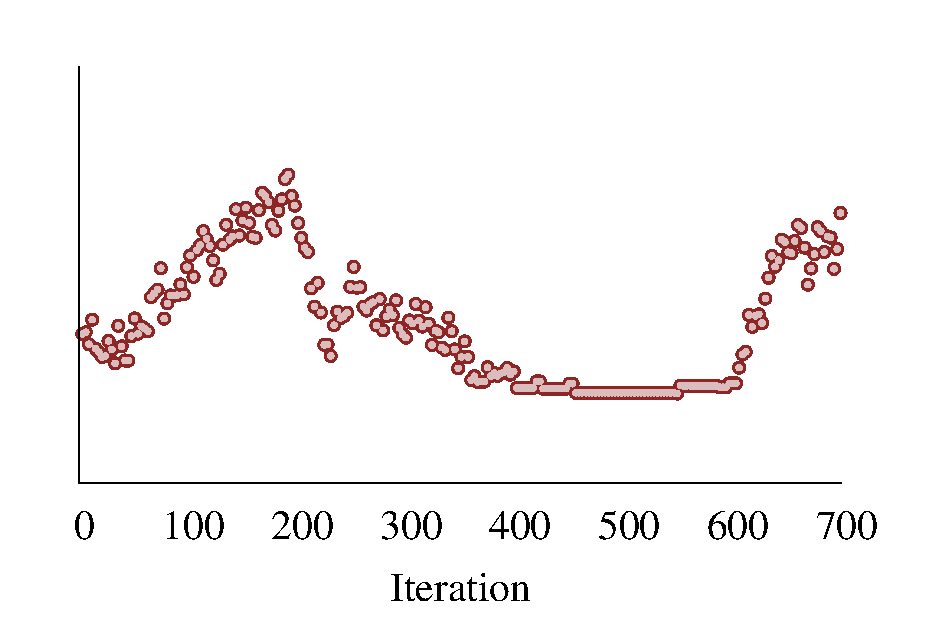
\includegraphics[width=6cm]{funnel_trace3.eps}};
\end{tikzpicture}
}
\caption{In practice, pathological regions of the typical set usually
cause Markov chains to get ``stuck''.  (a) Initially the Markov chain 
explores well-behaved regions of the typical set, avoiding the 
pathological neighborhood entirely and biasing Markov chain
Monte Carlo estimators.  (b) If the Markov chain is run long enough
then it will get stuck near the boundary of the pathological region, 
slowly correcting the Markov chain Monte Carlo estimators.  (c) 
Eventually the Markov chain escapes and explores the rest of 
the typical set.  This process repeats, causing the resulting 
estimators to oscillate around the true expectations in an unstable 
fashion.}
\label{fig:pathological exploration}
\end{figure*}

Ultimately this behavior results in estimators that oscillate 
around the true expectations.  Asymptotically the oscillations
average out to the true values, but that balance is delicate and
any finite time estimator will suffer from substantial biases.

Whether or not features of the target distribution become
pathological depends on how the Markov transition kernel
interacts with the target distribution.  Some transition kernels
are more robust than others and some can achieve robust
performance with careful tuning of auxiliary kernel parameters.
 
\subsubsection{MCMC in Practice}

In order to guarantee that we will not suffer from pathological
behavior we have to demonstrate strong \emph{ergodicity}
conditions that ensure the Markov chain not only explores
the typical set but does so sufficiently fast without being
hampered by pathological neighborhoods.  In most cases
we need to establish \emph{geometric ergodicity}.

Although we can identify generic features that often prevent
geometric ergodicity, determining whether or not a particular
Markov chain will exhibit pathological behavior when 
targeting a particular distribution is almost always infeasible
for nontrivial problems.  Moreover, there are no sufficient
conditions that we can use to establish geometric ergodicity
empirically.  Instead we have to rely on necessary conditions 
to provide any evidence that we can trust the resulting Markov 
chain Monte Carlo estimators.

Consequently we have to take great care when implementing
Markov chain Monte Carlo, and to maximize robust performance
we proceed in three stages.

\vspace{2mm}
\noindent \emph{Warmup}
\vspace{2mm}

We begin with \emph{warmup}, where we initialize multiple
chains from multiple, ideally diffuse, points in the sample space
and run long enough for them to converge to the typical set.
Because we do not include these warmup samples in any
Markov chain Monte Carlo estimators, we can also use this
period to adaptively tune any parameters in the Markov 
kernel without biasing our estimates.

Historically this stage has usually been called \emph{burn-in},
but we find that terminology inappropriate for Markov chain
Monte Carlo.  The problem is that burn-in is a process of 
stress-testing a system to identify and replace any failing
components.  In Markov chain Monte Carlo, however, any
misbehaving chains identify pathological behavior that is
biasing all of the chains and should very much not be ignored!
Because of this potentially-confusing, false analogy we use the
term warmup.

\vspace{2mm}
\noindent \emph{Sampling}
\vspace{2mm}

Once warmup as finished we begin a sampling phase where
we run the Markov chain and save all of the resulting samples
to construct Markov chain Monte Carlo estimators.

\vspace{2mm}
\noindent \emph{Evaluation}
\vspace{2mm}

Once both warmup and sampling have completed we can
search for any signs of pathological behavior and, if we
can't find any, move on to computing any desired estimator.

For what kind of pathological behavior should we be looking?
If we don't run warmup long enough for all of the Markov
chains to converge then not all of the Markov chains will look 
the same.  Similarly, any pathological regions in the typical set 
will bias the Markov chains in different ways.  Consequently a 
necessary condition for robust Markov chain Monte Carlo 
estimators is that each Markov chain appears identical.  In theory
we can quantify the homogeneity of our ensemble of Markov chains 
with the \emph{potential scale reduction factor} and in practice we
can estimate the potential scale reduction factor with the $\hat{R}$
statistic.

In addition to $\hat{R}$, specific Markov transitions may admit
their own, unique diagnostics sensitive to various pathologies
that can frustrate geometric ergodicity.

If we are confident that our Markov chains are exploring without
obstruction then we can finally compute Markov chain Monte
Carlo estimators using the samples generated in the sampling
phase.  If we also estimate the variances and autocorrelations
of each function then we can also quantify the error of these
estimates using an estimate of the Markov chain Monte Carlo
Standard Error.

\chapter{Bayesian Inference}

With a foundation of probability theory we are now ready to
formally define concepts like measurement, inference, and 
decision making.  Here we consider a Bayesian approach
to these ideas, although the same foundation is also critical
for constructing a frequentist approach.

We begin by defining measurements and what we want
to learn from those measurements, and then consider how
we approximate that system in practice with an abstract
mathematical model.  Once we have defined a model we
can define how we learn from that model and then how
we make decisions with that model.

\subsection{Measurements}

The basic assumption underlying inference is that there is some
observable process that we would like to understand, or at least
some latent process that has observable consequences.

These observable consequences manifest as logical statements,
but in practice we can observe only variable measurements
of those statements.  In order to formalize these concepts we
assume that this variability is sufficiently well-behaved that we
can describe it with probability theory.  More formally, we assume
that the process under consideration defines a probability 
distribution, $\PP_{D}$ over some measurement space, $D$, 
with measurements defined as events in the corresponding
event space.  

Although we have assumed the existence of a \emph{data
generating process}, $\PP_{D}$, we have intentionally not
assumed any philosophical interpretation of it.  In particular, we
are indifferent to the ultimate source of the variability in the
measurements quantified by $\PP_{D}$: it could be some
ontological variability inherent to the system or just some
epistemological variability due to our ignorance of the underlying 
system.  The only assumption we have made is that the
measurements are repeatable and variable, and that this
variability is sufficiently well-behaved to be described by a 
mathematical model. 

Although we can assume the existence of a data generating 
process, we don't know anything about it until we start making 
measurements.  An infinite number of measurements would 
certainly inform us of the data generating process exactly,
but measurements are expensive and in practice we have
to learn about the data generating process from only a few
measurements, if not just a single measurement. \emph{Inference}
is the process of learning about the data generating process
using only a finite number measurements.  

\subsection{Big Worlds and Small Worlds}

If we want to learn about the data generating process we have
to consider all possible data generating process we could
encounter or, equivalently, all possible probability distributions
over the sample space, $D$.  We refer to this massive set, $\mathcal{P}_{D}$
as the \emph{the big world} (Figure \ref{fig:big_world}).  

\begin{figure*}
\centering
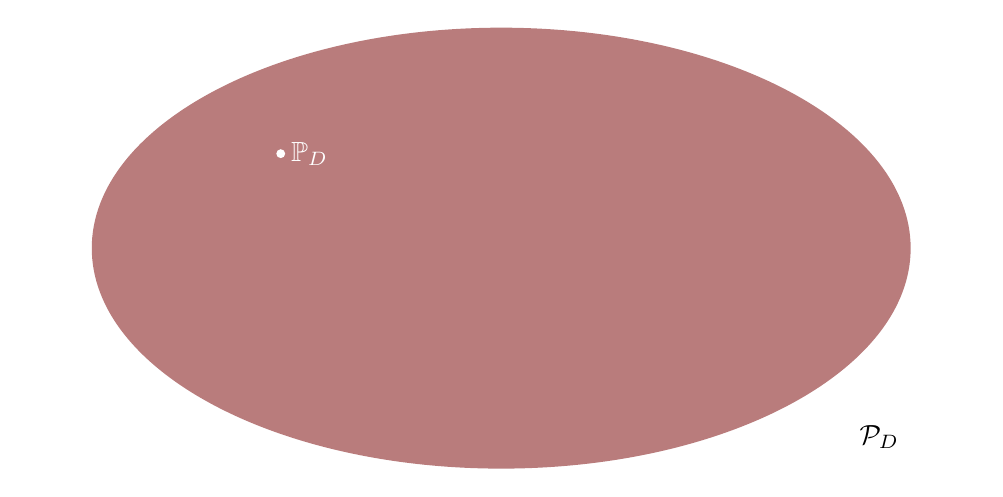
\begin{tikzpicture}[scale=0.40, thick]

  \draw[color=white] (-15, 0) -- (15, 0);

  \fill[mid] (0, 0) ellipse (13 and 7);
  \node at (12, -6) {$\mathcal{P}_{D}$};
  
  \fill[color=white] (-7, 3) circle (4pt)
  node[right, color=white] {$\PP_{D}$};
  
\end{tikzpicture}
\caption{Once we have defined a measurement space, $D$, the latent data
generating process, $\PP_{D}$ can be found in the space of all possible
data generating processes over $D$, $\mathcal{P}_{D}$.
}
\label{fig:big_world}
\end{figure*}

The big world is much too ungainly to be even well-defined in practice, 
let alone exhaustively explored.  Instead we have to limit our consideration 
to only a subset of probability distributions over the measurement space 
called a \emph{small world}, $\Theta \subset \mathcal{P}_{D}$ 
(Figure \ref{fig:small_worlds}a).

Each point in the small world, $\theta \in \Theta$, identifies a unique 
probability distribution over data.  Consequently the small world is 
equivalent to a probability distribution over the measurement space
conditioned on the small world,
%
\begin{align*}
\mathbb{L}
&: \EV{D} \times \Theta \rightarrow \left[0, 1 \right] \\
&\quad \left( E_{D}, \theta \right) \;\; \mapsto 
\mathbb{L} \! \left[ E_{D} \mid \theta \right].
\end{align*}
%
This conditional probability distribution is also known as the 
\emph{likelihood}.

Regardless of how it is chosen, the assumption of any specific 
small world can have drastic limitations on inference.  Because any
small world is typically only a shallow approximation of reality,
for example, it is unlikely to contain the latent data generating
process (Figure \ref{fig:small_worlds}b).  Consequently even ideal
inferences are subject to error, and the utility of any inference
always depends on the viability of our assumptions.

\begin{figure*}
\centering
%
\subfigure[]{
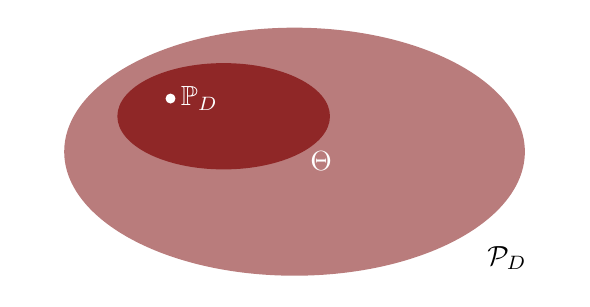
\begin{tikzpicture}[scale=0.225, thick]
  
  \draw[color=white] (-15, 0) -- (15, 0);
  
  \fill[mid] (0, 0) ellipse (13 and 7);
  \node at (12, -6) {$\mathcal{P}_{D}$};
  
  \fill[dark] (-4, 2) ellipse (6 and 3);
  \node[color=white] at (1.5, -0.5) {$\Theta$};
  
  \fill[color=white] (-7, 3) circle (8pt)
  node[right, color=white] {$\PP_{D}$};
  
\end{tikzpicture}
}
\subfigure[]{
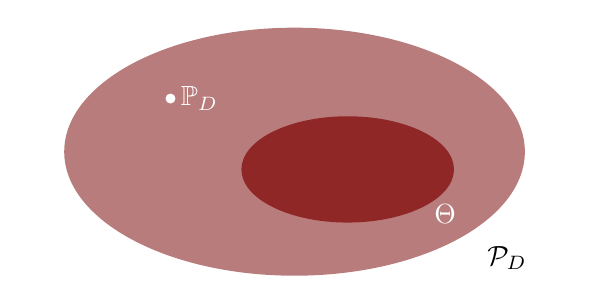
\begin{tikzpicture}[scale=0.225, thick]

  \draw[color=white] (-15, 0) -- (15, 0);

  \fill[mid] (0, 0) ellipse (13 and 7);
  \node at (12, -6) {$\mathcal{P}_{D}$};
  
  \fill[dark] (3, -1) ellipse (6 and 3);
  \node[color=white] at (8.5, -3.5) {$\Theta$};
  
  \fill[color=white] (-7, 3) circle (8pt)
  node[right, color=white] {$\PP_{D}$};
  
\end{tikzpicture}
}
\caption{Practical inference requires the selection of a distinguished subset 
of data generating processes called a small world, $\Theta$, that (a) may or 
(b) may not contain the latent data generating process, $\PP_{D}$.  The 
Boxian philosophy of ``all models are wrong but some are useful'' asserts 
that the former is impossible in practical problems, but even in the latter
the probability distributions in the small world may provide useful approximations 
of $\PP_{D}$.
}
\label{fig:small_worlds}
\end{figure*}

\subsection{Uncertainty And Learning In The Small World}

We have already used probability theory to quantify the variability of measurements,
but now we can also use probability theory to quantify our uncertainty about which
elements of the small world are good approximations to the latent data
generating process.  

The \emph{prior distribution}, $\PP_{\Theta}^{\mathrm{prior}}$, is a probability 
distribution over the small world that quantifies our initial uncertainty about 
which elements are most consistent with the latent data generating process.  
The information inherent in the prior distribution can come from previous 
measurements, theoretical constraints, or even elicitation of experts.  

Learning in the small world is the process of updating the prior distribution
with any information contained in the measurement to give a \emph{posterior
distribution}, $\PP_{\Theta}^{\mathrm{post}}$, that quantifies our uncertainty
about the small world after the measurement  (Figure \ref{fig:learning}).  The 
likelihood implicitly quantifies any information contained in a measurement and 
then the actual mechanism for this update is immediately given by probability 
theory.  It is most simply written in terms of probability density functions,
%
\begin{equation*}
p^{\mathrm{post}} \! \left( \theta \mid d \right)
\propto
L \! \left( d \mid \theta \right) p^{\mathrm{prior}} \! \left( \theta \right),
\end{equation*}
%
which can be recognized as the celebrated Bayes' Theorem.

Bayes' Theorem, however, is just a mathematical consequence of probability
theory and its appearance is an inevitability once we use probabilities to
quantify our uncertainty about the small world.  Ultimately, all of this
abstraction is just a means to formalize the intuition that \emph{what we know 
after a measurement is what we knew before the measurement plus any 
information contained in the measurement}.

\begin{figure*}
\centering
%
\subfigure[]{
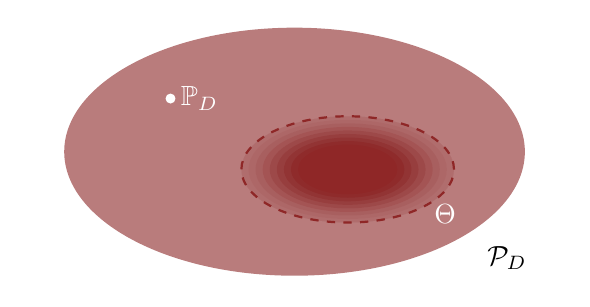
\begin{tikzpicture}[scale=0.225, thick]

  \draw[color=white] (-15, 0) -- (15, 0);

  \fill[mid] (0, 0) ellipse (13 and 7);
  \node at (12, -6) {$\mathcal{P}_{D}$};
  
  \draw[color=dark, dashed] (3, -1) ellipse (6 and 3);
  \node[color=white] at (8.5, -3.5) {$\Theta$};
  
  \fill[color=white] (-7, 3) circle (8pt)
  node[right, color=white] {$\PP_{D}$};
  
  \begin{scope}
    \clip (3, -1) ellipse (6 and 3);
    \foreach \i in {0, 0.05,..., 1} {
      \fill[opacity={exp(-5 * \i*\i)}, dark] (3, -1) ellipse ({8 * \i} and {4 * \i});      
    }
  \end{scope}
  
\end{tikzpicture}
}
%
\subfigure[]{
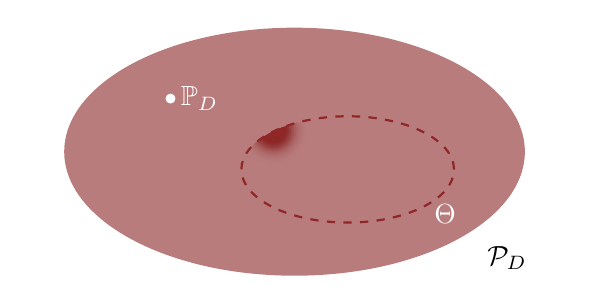
\begin{tikzpicture}[scale=0.225, thick]

  \draw[color=white] (-15, 0) -- (15, 0);

  \fill[mid] (0, 0) ellipse (13 and 7);
  \node at (12, -6) {$\mathcal{P}_{D}$};
  
  \draw[color=dark, dashed] (3, -1) ellipse (6 and 3);
  \node[color=white] at (8.5, -3.5) {$\Theta$};
  
  \fill[color=white] (-7, 3) circle (8pt)
  node[right, color=white] {$\PP_{D}$};
  
  \begin{scope}
    \clip (3, -1) ellipse (6 and 3);
    \foreach \i in {0, 0.05,..., 1} {
      \fill[opacity={exp(-5 * \i*\i)}, dark] (-1.2, 1.2) circle ({2 * \i});      
    }
  \end{scope}
  
\end{tikzpicture}
}
\caption{Inference in the small world is the process of updating
(a) a prior distribution quantifying our initial uncertainty about the small
world into (b) a posterior distribution quantifying our uncertainty about
the small world after incorporating any information in a measurement.
If all of our assumptions are viable then the posterior should concentrate
towards the latent data generating process, $\PP_{D}$.
}
\label{fig:learning}
\end{figure*}

\subsection{TODO: Decision Making in the Small World}

Now that we've quantified uncertainty we can make robust decisions.

Formalize with a risk/utility function, compute expected risk/utility, then
chose the decision that minimizes/maximizes the expected risk/utility.

\subsection{TODO: Bayesian Inference in Practice}

Model a prior and a likelihood.  Posterior is immediately given and
all statements about our system, including decisions, are given by
expectations.  As discussed above we have many options for
approximating those expectations in practice.

The biggest challenge in implementing Bayesian inference, then,
is the actual modeling of the prior and likelihood.  Much can be
said about both, but let's take a second to discuss one of the most
powerful means of methods of building small worlds: \emph{generative modeling}.  
Here we build up the small world
sequentially by modeling each state of the data generating process.
For example, we might build a small world for polling data by
modeling the sampling of an individual from a population and
then a series of non-responses based on the individual's demographics.
Or we might have a strong physical model, which we can wrap
in an equality complex measurement model to account for the
various systematic effects introduced in the measurement process.
Any such model will be an approximation to the true generative
process, but this perspective allows us to build better and better
approximations by adding more and more detail as necessary.
\textbf{Natural way to unite user intuition with explicit modeling.}
\textbf{More detail in examples, emphasizing modeling of
measurement process.}

\textbf{Constructive example mirroring the motivating example
in the introduction.}

\textbf{Generative models as a way to define small worlds with
disintegrations.  Does not necessarily imply causal structure
but the more casual structure the better!}

\subsection{TODO: Checking Model Assumptions with Predictive Performance}

Checking model assumptions with posterior predictive checks.

\begin{figure*}
\centering
%
\subfigure[]{
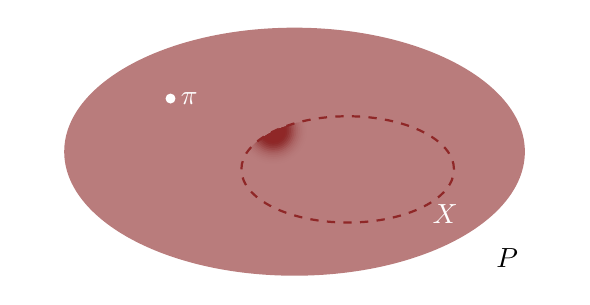
\begin{tikzpicture}[scale=0.225, thick]
  \draw[color=white] (-15, 0) -- (15, 0);

  \fill[mid] (0, 0) ellipse (13 and 7);
  \node at (12, -6) {$P$};
  
  \draw[color=dark, dashed] (3, -1) ellipse (6 and 3);
  \node[color=white] at (8.5, -3.5) {$X$};
  
  \fill[color=white] (-7, 3) circle (8pt)
  node[right, color=white] {$\pi$};
  
  \begin{scope}
    \clip (3, -1) ellipse (6 and 3);
    \foreach \i in {0, 0.05,..., 1} {
      \fill[opacity={exp(-5 * \i*\i)}, dark] (-1.2, 1.2) circle ({2 * \i});      
    }
  \end{scope} 
\end{tikzpicture}
}
%
\subfigure[]{
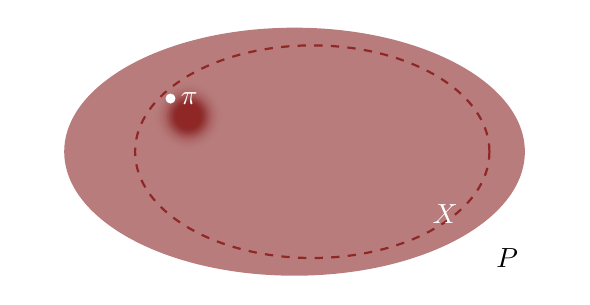
\begin{tikzpicture}[scale=0.225, thick]
  \draw[color=white] (-15, 0) -- (15, 0);

  \fill[mid] (0, 0) ellipse (13 and 7);
  \node at (12, -6) {$P$};
  
  \draw[color=dark, dashed] (1, 0) ellipse (10 and 6);
  \node[color=white] at (8.5, -3.5) {$X$};
  
   \begin{scope}
    \clip (1, 0) ellipse (10 and 6);
    \foreach \i in {0, 0.05,..., 1} {
      \fill[opacity={exp(-5 * \i*\i)}, dark] (-6, 2) circle ({2 * \i});      
    }
  \end{scope}
  
  \fill[color=white] (-7, 3) circle (8pt)
  node[right, color=white] {$\pi$};
\end{tikzpicture}
}
\caption{Cartoon of model updating.
}
\label{fig:model_updating}
\end{figure*}

\end{document}  